%%%%%%%%%%%%%%%%%%%%%%%%%%%%%%%%%%%%%%%%%
% Tufte-Style Book (Documentation Template)
% LaTeX Template
% Version 1.0 (5/1/13)
%
% This template has been downloaded from:
% http://www.LaTeXTemplates.com
%
% Original author:
% The Tufte-LaTeX Developers (tufte-latex.googlecode.com)
%
% License:
% Apache License (Version 2.0)
%
% IMPORTANT NOTE:
% In addition to running BibTeX to compile the reference list from the .bib
% file, you will need to run MakeIndex to compile the index at the end of the
% document.
%
%%%%%%%%%%%%%%%%%%%%%%%%%%%%%%%%%%%%%%%%%

%----------------------------------------------------------------------------------------
%	PACKAGES AND OTHER DOCUMENT CONFIGURATIONS
%----------------------------------------------------------------------------------------

\documentclass{tufte-book} % Use the tufte-book class which in turn uses the tufte-common class

\hypersetup{colorlinks} % Comment this line if you don't wish to have colored links

\usepackage{microtype} % Improves character and word spacing

\usepackage{lipsum} % Inserts dummy text

\usepackage{booktabs} % Better horizontal rules in tables

\usepackage{graphicx} % Needed to insert images into the document
\graphicspath{{graphics/}} % Sets the default location of pictures
\setkeys{Gin}{width=\linewidth,totalheight=\textheight,keepaspectratio} % Improves figure scaling

\usepackage{fancyvrb} % Allows customization of verbatim environments
\fvset{fontsize=\normalsize} % The font size of all verbatim text can be changed here

\newcommand{\hangp}[1]{\makebox[0pt][r]{(}#1\makebox[0pt][l]{)}} % New command to create parentheses around text in tables which take up no horizontal space - this improves column spacing
\newcommand{\hangstar}{\makebox[0pt][l]{*}} % New command to create asterisks in tables which take up no horizontal space - this improves column spacing

\usepackage{xspace} % Used for printing a trailing space better than using a tilde (~) using the \xspace command

\newcommand{\monthyear}{\ifcase\month\or January\or February\or March\or April\or May\or June\or July\or August\or September\or October\or November\or December\fi\space\number\year} % A command to print the current month and year

\newcommand{\openepigraph}[2]{ % This block sets up a command for printing an epigraph with 2 arguments - the quote and the author
\begin{fullwidth}
\sffamily\large
\begin{doublespace}
\noindent\allcaps{#1}\\ % The quote
\noindent\allcaps{#2} % The author
\end{doublespace}
\end{fullwidth}
}

\newcommand{\blankpage}{\newpage\hbox{}\thispagestyle{empty}\newpage} % Command to insert a blank page

\usepackage{units} % Used for printing standard units

\newcommand{\hlred}[1]{\textcolor{Maroon}{#1}} % Print text in maroon
\newcommand{\hangleft}[1]{\makebox[0pt][r]{#1}} % Used for printing commands in the index, moves the slash left so the command name aligns with the rest of the text in the index
\newcommand{\hairsp}{\hspace{1pt}} % Command to print a very short space
\newcommand{\ie}{\textit{i.\hairsp{}e.}\xspace} % Command to print i.e.
\newcommand{\eg}{\textit{e.\hairsp{}g.}\xspace} % Command to print e.g.
\newcommand{\na}{\quad--} % Used in tables for N/A cells
\newcommand{\measure}[3]{#1/#2$\times$\unit[#3]{pc}} % Typesets the font size, leading, and measure in the form of: 10/12x26 pc.
\newcommand{\tuftebs}{\symbol{'134}} % Command to print a backslash in tt type in OT1/T1

\providecommand{\XeLaTeX}{X\lower.5ex\hbox{\kern-0.15em\reflectbox{E}}\kern-0.1em\LaTeX}
\newcommand{\tXeLaTeX}{\XeLaTeX\index{XeLaTeX@\protect\XeLaTeX}} % Command to print the XeLaTeX logo while simultaneously adding the position to the index

\newcommand{\doccmdnoindex}[2][]{\texttt{\tuftebs#2}} % Command to print a command in texttt with a backslash of tt type without inserting the command into the index

\newcommand{\doccmddef}[2][]{\hlred{\texttt{\tuftebs#2}}\label{cmd:#2}\ifthenelse{\isempty{#1}} % Command to define a command in red and add it to the index
{ % If no package is specified, add the command to the index
\index{#2 command@\protect\hangleft{\texttt{\tuftebs}}\texttt{#2}}% Command name
}
{ % If a package is also specified as a second argument, add the command and package to the index
\index{#2 command@\protect\hangleft{\texttt{\tuftebs}}\texttt{#2} (\texttt{#1} package)}% Command name
\index{#1 package@\texttt{#1} package}\index{packages!#1@\texttt{#1}}% Package name
}}

\newcommand{\doccmd}[2][]{% Command to define a command and add it to the index
\texttt{\tuftebs#2}%
\ifthenelse{\isempty{#1}}% If no package is specified, add the command to the index
{%
\index{#2 command@\protect\hangleft{\texttt{\tuftebs}}\texttt{#2}}% Command name
}
{%
\index{#2 command@\protect\hangleft{\texttt{\tuftebs}}\texttt{#2} (\texttt{#1} package)}% Command name
\index{#1 package@\texttt{#1} package}\index{packages!#1@\texttt{#1}}% Package name
}}

% A bunch of new commands to print commands, arguments, environments, classes, etc within the text using the correct formatting
\newcommand{\docopt}[1]{\ensuremath{\langle}\textrm{\textit{#1}}\ensuremath{\rangle}}
\newcommand{\docarg}[1]{\textrm{\textit{#1}}}
\newenvironment{docspec}{\begin{quotation}\ttfamily\parskip0pt\parindent0pt\ignorespaces}{\end{quotation}}
\newcommand{\docenv}[1]{\texttt{#1}\index{#1 environment@\texttt{#1} environment}\index{environments!#1@\texttt{#1}}}
\newcommand{\docenvdef}[1]{\hlred{\texttt{#1}}\label{env:#1}\index{#1 environment@\texttt{#1} environment}\index{environments!#1@\texttt{#1}}}
\newcommand{\docpkg}[1]{\texttt{#1}\index{#1 package@\texttt{#1} package}\index{packages!#1@\texttt{#1}}}
\newcommand{\doccls}[1]{\texttt{#1}}
\newcommand{\docclsopt}[1]{\texttt{#1}\index{#1 class option@\texttt{#1} class option}\index{class options!#1@\texttt{#1}}}
\newcommand{\docclsoptdef}[1]{\hlred{\texttt{#1}}\label{clsopt:#1}\index{#1 class option@\texttt{#1} class option}\index{class options!#1@\texttt{#1}}}
\newcommand{\docmsg}[2]{\bigskip\begin{fullwidth}\noindent\ttfamily#1\end{fullwidth}\medskip\par\noindent#2}
\newcommand{\docfilehook}[2]{\texttt{#1}\index{file hooks!#2}\index{#1@\texttt{#1}}}
\newcommand{\doccounter}[1]{\texttt{#1}\index{#1 counter@\texttt{#1} counter}}

\usepackage{makeidx} % Used to generate the index
\makeindex % Generate the index which is printed at the end of the document

% This block contains a number of shortcuts used throughout the book
\newcommand{\vdqi}{\textit{VDQI}\xspace}
\newcommand{\ei}{\textit{EI}\xspace}
\newcommand{\ve}{\textit{VE}\xspace}
\newcommand{\be}{\textit{BE}\xspace}
\newcommand{\VDQI}{\textit{The Visual Display of Quantitative Information}\xspace}
\newcommand{\EI}{\textit{Envisioning Information}\xspace}
\newcommand{\VE}{\textit{Visual Explanations}\xspace}
\newcommand{\BE}{\textit{Beautiful Evidence}\xspace}
\newcommand{\TL}{Tufte-\LaTeX\xspace}

%----------------------------------------------------------------------------------------
%	BOOK META-INFORMATION
%----------------------------------------------------------------------------------------

\title{Principled Optimization of Dynamic Neural Networks} % Title of the book

\author[Jared Roesch]{Jared Roesch}

% \publisher{Publisher of This Book} % Publisher

%----------------------------------------------------------------------------------------

\usepackage{xspace}
\usepackage{amsmath}
\usepackage{bcprules}
\usepackage{color}
\usepackage{graphicx}
\graphicspath{.}
\usepackage{alltt}
\usepackage{lineno}
\usepackage{proof}
\usepackage{verbatim}
\usepackage{xcolor}
\usepackage{tikz}
\usepackage{minted}
\def\OPTIONConf{1}%
\usepackage{tabularx}
\usepackage{longtable}
\usepackage{booktabs}
% \usepackage{caption}
% \usepackage{subcaption}
\usepackage{joshuadunfield}
% \usepackage{natbib}
% \usepackage{enumitem}
% \usepackage[nounderscore]{syntax}
\usepackage{tabu}
\usepackage{amssymb}
\usepackage{mathtools}

% \usepackage{txfonts}

\newcommand{\makered}[1]{\textcolor{red}{#1}}
\newcommand{\redbold}[1]{\makered{\textbf{#1}}}
\newcommand{\makegreen}[1]{\textcolor{green}{#1}}
\newcommand{\greenbold}[1]{\makegreen{\textbf{#1}}}
\newcommand{\note}[1]{\redbold{[#1]}}
\newcommand{\nnvm}[0]{NNVM\xspace}
\newcommand{\tvm}[0]{TVM\xspace}
% \newcommand{\relay}[0]{Relay}
\newcommand{\relay}[0]{InterNeuron\xspace}
\newcommand{\vta}[0]{VTA\xspace}
% \newcommand{\kwd}[1]{\,\fcolorbox{gray!30}{gray!30}{\texttt{#1}}\,}
% \newcommand{\kwd}[1]{\texttt{#1}}
% TODO: doesn't seem to produce the exact color. also contrast is a little low
\definecolor{sampldark}{RGB}{72, 71, 135}
\definecolor{uwpurp}{RGB}{51, 0, 111}
\definecolor{uwpurplight}{RGB}{94, 0, 204}
\newcommand{\kwd}[1]{\textcolor{uwpurplight}{\texttt{#1}}}
\def\checkmark{\tikz\fill[scale=0.4](0,.35) -- (.25,0) -- (1,.7) -- (.25,.15) -- cycle;}
\newcommand{\Cross}{\tikz [x=1.4ex,y=1.4ex,line width=.2ex] \draw (0,0) -- (1,1) (0,1) -- (1,0);}%

% https://math.berkeley.edu/~gbergman/misc/hacks/langl_rangl.html
\usepackage{graphics}
\newcommand{\langl}{\begin{picture}(4.5,7)
\put(1.1,2.5){\rotatebox{60}{\line(1,0){5.5}}}
\put(1.1,2.5){\rotatebox{300}{\line(1,0){5.5}}}
\end{picture}}
\newcommand{\rangl}{\begin{picture}(4.5,7)
\put(.9,2.5){\rotatebox{120}{\line(1,0){5.5}}}
\put(.9,2.5){\rotatebox{240}{\line(1,0){5.5}}}
\end{picture}}

\usepackage{todonotes}
\newcommand{\jgr}[1]{\todo[color=blue, size=\tiny]{#1}}
\newcommand{\jmp}[1]{\todo[color=green, size=\tiny]{#1}}
\newcommand{\ssl}[1]{\todo[color=yellow, size=\tiny]{#1}}

\newcommand{\jdiff}[2]{\redbold{#1}\greenbold{Jared: #2}}

\newcommand{\CaptionLabel}[2]{
  \caption{#1}
  \label{#2}}

% BNF
\newcommand{\is}[2][]{&::=&#2\ifthenelse{\equal{#1}{}}{}{&\text{(#1)}}}
\newcommand{\isEtc}{\is{\cdots}}
\newcommand{\inlineAlt}{~\vert~}
\newcommand{\alt}[2][]{\\&&\vert&#2\ifthenelse{\equal{#1}{}}{}{&\text{(#1)}}}
\newcommand{\altEtc}{\\&&\vdots}
\newcommand{\altSpace}[3]{\\[#1]&&\vert&#3\ifthenelse{\equal{#2}{}}{}{&\text{(#2)}}}
\newcommand{\grammarname}[1]{\textit{#1}}
\newcommand{\grammarword}[1]{\texttt{#1}}
\newcommand{\op}{\grammarname{op}}
\newcommand{\gvar}{\kwd{@}\grammarname{g}}
\newcommand{\type}{\grammarname{$\tau$}}
\newcommand{\expr}{\grammarname{e}}
\newcommand{\lvar}{\kwd{\%}\grammarname{l}}
\newcommand{\graphVar}{\kwd{\%}\grammarword{graph}}
\newcommand{\real}{\grammarname{r}}
\newcommand{\bool}{\grammarname{b}}
\newcommand{\nat}{\grammarname{n}}
\newcommand{\Item}{\grammarname{i}}
\newcommand{\defn}{\grammarword{def}}
\newcommand{\rettype}{\kwd{$\rightarrow$}\ \type}
\newcommand{\seq}[1]{#1\kwd{,}\ \ldots \kwd{,}\ #1}
\newcommand{\relations}{\kwd{where}\ \seq{\type}}
\newcommand{\tyvar}{\grammarname{tv}}
\newcommand{\tyParam}{\grammarword{T}}
\newcommand{\typarams}{\grammarword{tyParams}}
\newcommand{\typeanno}{\kwd{:}\, \type}
\newcommand{\kind}{k}
\newcommand{\kindanno}{\kwd{:}\, \kind}
\newcommand{\maybe}[1]{\texttt{(}#1\texttt{)?}}
\newcommand{\atLeastZero}[1]{\texttt{(}#1\texttt{)*}}
\newcommand{\atLeastOne}[1]{\texttt{(}#1\texttt{)+}}
\newcommand{\body}[1]{\kwd{\{} #1 \kwd{\}}}
\newcommand{\param}{\grammarword{x}}
\newcommand{\params}{\grammarword{params}}
\newcommand{\tyargs}{\kwd{$\langl$} \seq{\type} \kwd{$\rangl$}}
\newcommand{\args}{\kwd{(} \seq{\expr} \kwd{)}}
\newcommand{\bnfrule}[2]{\textsf{#1} & #2}
\newcommand{\basetype}{\grammarname{bt}}
\newcommand{\shape}{\grammarname{s}}
\newcommand{\patt}{\grammarname{p}}
\newcommand{\wildcard}{\kwd{\_}}
\newcommand{\typename}{\grammarname{tn}}
\newcommand{\rName}{\grammarword{name}}
\newcommand{\rTrue}{\kwd{true}}
\newcommand{\rFalse}{\kwd{false}}
\newcommand{\rFnRule}{\begin{split}
  \kwd{fn}\ &\maybe{\rTyParamsRule}\\&\rParamsRule\ \maybe{\rettype}\\&\body{\expr}
\end{split}}
\newcommand{\rDefnRule}{\begin{split}
  \kwd{def}\ \gvar&\maybe{\rTyParamsRule}\\&\rParamsRule\ \maybe{\rettype}\\&\maybe{\relations}\ \body{\expr}
\end{split}}
\newcommand{\rTupRule}{\kwd{(} \seq{\expr} \kwd{)}}
\newcommand{\rTupProjRule}{e \kwd{.} \nat}
\newcommand{\rIfElse}[3]{\kwd{if}\ \kwd{(} #1 \kwd{)}\ \body{#2}\ \kwd{else}\
\body{#3}}
\newcommand{\rLetRule}{\kwd{let}\ \lvar\ \maybe{\typeanno}\ \kwd{=}\ \expr \kwd{;}\ \expr}
\newcommand{\rAnonLetRule}{\expr \kwd{;}\ \expr}
\newcommand{\rGraphLetRule}{\graphVar\ \kwd{=}\ \expr \kwd{;}\ \expr}
\newcommand{\rLet}[4]{\kwd{let}\ #1\ifthenelse{\equal{#2}{}}{}{\ \kwd{:}\, #2}\ \kwd{=}\ #3 \kwd{;}\ifthenelse{\equal{#4}{}}{}{\ #4}}
\newcommand{\rTyParamsRule}{\kwd{$\langl$} \seq{\tyParam} \kwd{$\rangl$}}
\newcommand{\rParamsRule}{\kwd{(} \seq{\param} \kwd{)}}
\newcommand{\rParamRule}{\lvar\ \maybe{\typeanno}}
\newcommand{\rParam}[2]{#1\kwd{:}\ #2}
\newcommand{\rTyParamRule}{\tyvar\ \maybe{\kindanno}}
\newcommand{\typedef}{\grammarword{type}}
\newcommand{\rTypeDefRule}{\begin{aligned}
  &\kwd{type}\ \typename \rTyParamsRule\ \kwd{\{}\\
  &\quad\kwd{|}\ \op\kwd{(} \seq{\type} \kwd{)}\\
  &\quad \vdots\\
  &\quad\kwd{|}\ \op\kwd{(} \seq{\type} \kwd{)}\\
  &\kwd{\}}
\end{aligned}}
\newcommand{\rMatchRule}{\begin{aligned}
  &\kwd{match}\ \kwd{(} \expr \kwd{)}\ \kwd{\{}\\
  &\quad\kwd{|}\ \patt\ \kwd{$\rightarrow$}\ \expr \\
  &\quad \vdots\\
  &\quad\kwd{|}\ \patt\ \kwd{$\rightarrow$}\ \expr \\
  &\kwd{\}}
\end{aligned}}
\newcommand{\program}{\grammarword{program}}

% Draw a pentagram and summon Knuth for a varargs intercalate macro.
\makeatletter
\newcommand{\intercalate}[4]{%
    #2#4\intercCheckNext{#1}{#3}}
\newcommand{\intercCheckNext}[2]{\@ifnextchar\bgroup{\intercGobbleNext{#1}{#2}}{}}
\newcommand{\intercGobbleNext}[3]{#1 #3\@ifnextchar\bgroup{\intercGobbleNext{#1}{#2}}{#2}}
\makeatother

\newcommand{\rTuple}{%
    \intercalate{\kwd{,}}{\kwd{(}}{\kwd{)}}}

% typecheck
\newcommand{\typecheck}[4]{#1 ; #2 \entails #3 : #4}
\newcommand{\typeCtx}{\grammarname{$\Delta$}}
\newcommand{\varCtx}{\grammarname{$\Gamma$}}

% semantics
\newcommand{\rstep}[2]{#1 \Rightarrow #2}
\newcommand{\rstate}[3]{#1; #2\colon #3}
\newcommand{\rheap}{\grammarname{$\Gamma$}}
\newcommand{\rnamespace}{\grammarname{$\Delta$}}

% AD Figure
\newcommand{\pluseq}{\mathrel{+}=}
\newcommand{\revv}[1]{\overset{\leftharpoonup} #1}
\newcommand{\sens}[1]{\overset{\leftharpoondown} #1}
\newcommand{\bper}[1]{\overline{#1}}

\newcommand{\affiliation}[1]{//\texttt{#1}}
\newcommand{\email}[1]{//\texttt{#1}}


\begin{document}

\frontmatter

%----------------------------------------------------------------------------------------
%	EPIGRAPH
%----------------------------------------------------------------------------------------

% \thispagestyle{empty}
% \openepigraph{The public is more familiar with bad design than good design. It is, in effect, conditioned to prefer bad design, because that is what it lives with. The new becomes threatening, the old reassuring.}{Paul Rand, {\itshape Design, Form, and Chaos}}
% \vfill
% \openepigraph{A designer knows that he has achieved perfection not when there is nothing left to add, but when there is nothing left to take away.}{Antoine de Saint-Exup\'{e}ry}
% \vfill
% \openepigraph{\ldots the designer of a new system must not only be the implementor and the first large-scale user; the designer should also write the first user manual\ldots If I had not participated fully in all these activities, literally hundreds of improvements would never have been made, because I would never have thought of them or perceived why they were important.}{Donald E. Knuth}

%----------------------------------------------------------------------------------------

\maketitle % Print the title page

%----------------------------------------------------------------------------------------
%	COPYRIGHT PAGE
%----------------------------------------------------------------------------------------

\newpage
\begin{fullwidth}
~\vfill
\thispagestyle{empty}
\setlength{\parindent}{0pt}
\setlength{\parskip}{\baselineskip}
Copyright \copyright\ \the\year\ \thanklessauthor

\par\smallcaps{Published by \thanklesspublisher}

\par\smallcaps{tufte-latex.googlecode.com}

\par Licensed under the Apache License, Version 2.0 (the ``License''); you may not use this file except in compliance with the License. You may obtain a copy of the License at \url{http://www.apache.org/licenses/LICENSE-2.0}. Unless required by applicable law or agreed to in writing, software distributed under the License is distributed on an \smallcaps{``AS IS'' BASIS, WITHOUT WARRANTIES OR CONDITIONS OF ANY KIND}, either express or implied. See the License for the specific language governing permissions and limitations under the License.\index{license}

\par\textit{First printing, \monthyear}
\end{fullwidth}

\newpage
Abstract ...

%----------------------------------------------------------------------------------------

\tableofcontents % Print the table of contents

%----------------------------------------------------------------------------------------

\listoffigures % Print a list of figures

%----------------------------------------------------------------------------------------

\listoftables % Print a list of tables

%----------------------------------------------------------------------------------------
%	DEDICATION PAGE
%----------------------------------------------------------------------------------------

\cleardoublepage
~\vfill
\begin{doublespace}
\noindent\fontsize{18}{22}\selectfont\itshape
\nohyphenation
Dedicated to those who appreciate \LaTeX{} and the work of \mbox{Edward R.~Tufte} and \mbox{Donald E.~Knuth}.
\end{doublespace}
\vfill
\vfill


\noindent For example,
\begin{docspec}
\doccmdnoindex{documentclass}[symmetric,justified,marginals=raggedouter]\{tufte-book\}
\end{docspec}
will set the body text of the document to be fully justified and all of the margin material (sidenotes, margin notes, captions, and citations) to be flush against the body text with ragged outer edges.

\newthought{The font and style} of the marginal material may also be modified using the following commands:

\begin{docspec}
\doccmd{setsidenotefont}\{\docopt{font commands}\}\\
\doccmd{setcaptionfont}\{\docopt{font commands}\}\\
\doccmd{setmarginnotefont}\{\docopt{font commands}\}\\
\doccmd{setcitationfont}\{\docopt{font commands}\}
\end{docspec}

The \doccmddef{setsidenotefont} sets the font and style for sidenotes, the \doccmddef{setcaptionfont} for captions, the \doccmddef{setmarginnotefont} for margin notes, and the \doccmddef{setcitationfont} for citations. The \docopt{font commands} can contain font size changes (e.g., \doccmdnoindex{footnotesize}, \doccmdnoindex{Huge}, etc.), font style changes (e.g., \doccmdnoindex{sffamily}, \doccmdnoindex{ttfamily}, \doccmdnoindex{itshape}, etc.), color changes (e.g., \doccmdnoindex{color}\texttt{\{blue\}}), and many other adjustments.

If, for example, you wanted the captions to be set in italic sans serif, you could use:
\begin{docspec}
\doccmd{setcaptionfont}\{\doccmdnoindex{itshape}\doccmdnoindex{sffamily}\}
\end{docspec}

\chapter{Introduction}
\label{ch:intro}

Traditionally, machine learning algorithms were carefully engineered by humans
  in order to leverage limited data to obtain sufficient task performance.
During the Big Data era, these hand engineered algorithms were displaced by
  simpler algorithms applied to the abundantly available data~\citep{unreasonable}\footnote{"We don’t have better algorithms. We just have more data.” From "The Unreasonable Effectiveness of Data"}.
In order to scale these algorithms a number of frameworks were
  developed, most notably streaming and graph processing systems such as MapReduce and Spark.
In the early 2010s the emergence of deep learning changed the paradigm again
  replacing simple regular computation over streams with large batched-models
  composed of compute-hungry tensor computations.
The paradigm shift towards deep learning has started a trend of deploying models
  which are applied to more complex data (i.e., full text documents, images, videos, audio)
  process a greater quantity of data (millions of data points),
  and are more computationally and memory expensive to evaluate on a single datum (i.e., terra-flops of compute per sample).

This new generation of machine learning applications demanded a corresponding era of
  innovation in systems.
The first innovation in deep learning systems were
  ``deep learning frameworks"" such as TensorFlow and PyTorch.
These monolithic systems can execute a subset of deep learning models
  efficiently on a subset of the most popular hardware devices.
These systems provide good baseline performance, but often fail
  when straying from well-used models, and only support limited deployment strategies.
In particular TensorFlow's design was optimized for the distributed setting
  but provides a sub-optimal experience on a single node\footnote{In fact, I have been told by Google engineers they would jokingly refer to TensorFlow as TensorSlow in the early days.}.

Scaling frameworks to span the scope of all models and targets is a monumental endeavor
  requiring deep expertise often not found in conjunction with the skills of a
  machine learning engineer.
Even with the aid of a machine learning framework a machine learning engineer
  cannot write code that scales across the growing sea of
  models, operators, optimizations, and devices while maintaining state-of-the-art performance.
Frameworks only support a subset of programs, optimizations, and devices
  requiring large teams to extend frameworks for even relatively simple deviations
  from standard models.
Even when a team is able to get a model running observed performance often
  is lacking behind the performance of well trod workloads.
Large companies are able to mitigate this cost with raw capital expenditure
  but this puts smaller organizations and researchers on an unequal footing.
In the years after the introduction of frameworks it has become clear
  that automation is needed to both help smaller groups of engineers
  more effectively develop and deploy deep learning, and allow larger
  organizations to work effectively and efficiently.

From the early days of deep learning framework development researchers realized the
  potential for apply compilation to accelerate neural networks.~\footnote{Theano was applying
  compilation to deep learning as early as 2007.}
Modern frameworks borrowing ideas from the research community and previous
  experiences applying compilation began to introduce compilers into frameworks.

Deep learning compilers, systems for accelerating the execution deep learning via compilation,
 have made similar tradeoffs as frameworks by narrowly focusing on executing a subset
 currently popular of models on a subset of devices.
Designing a deep learning compiler even for this constrained subset is challenging.
For example,
  a popular state-of-the-art DL compiler,
  Google's XLA, can famously slow down programs on
  CPU instead of speeding them up.
Although non-intuitive this is a general challenge of applying compilation,
  it is not a silver bullet and may not provide uniform speedups across all input programs.
Compilers for deep learning~\citep{xla,jax,glow,tvm_osdi18,myia,fluxjl,lattner2020mlir} are
  a rapidly evolving area explored by both industrial and academic researchers.

A particular way in which deep learning frameworks have been narrowly focused
  is on the handling of static, feed-forward neural networks.
At the time of their design the deep learning revolution was occurring mostly
  in computer vision but had not fully taken over areas such as natural language processing (NLP).
Frameworks have enough general mechanisms that writing these models was mostly possibly
  a few years after their introduction.
Unfortunately the design of frameworks have severely limited the performance
  of programs that fall outside of the well-optimized footprint.
Furthermore the first-generation of compilers have been overfit
  for static compilation, they assume static control-flow, static tensor
  dimensions and no complex data structures.

This lack of support has manifested as a serious of ad-hoc extensions to
  both frameworks, deep learning runtimes, and

In particular I have spent the last several years focused on an under served problem:
  the representation,
  optimization,
  differentiation,
  and execution of \emph{dynamic neural networks}.
In this thesis I propose generalizing overspecialized
  compilation techniques applied to static dataflow graphs,
  the predominant programming model of deep learning,
  to fully dynamic neural networks.
These generalizations are powered by a simple insight:
  dynamic neural networks are just programs which manipulate tensors.
The challenge is constructing a representation that captures this generality
  in a principled manner, enabling state-of-the-art performance without limiting the programming model.
We realize a unified interface in the form of Relay: a set of systems and APIs designed
  to compose techniques across the stack to achieve state of the art performance.

Instead of building a single IR and compiler to rule them all\footnote{and in the darkness bind them}
  we carefully split the program optimization problem into a series of
  phases each focused on a specific optimization task.
This approach balances the tension between expressivity, composition
  and performance portability.
Part of my thesis work in graduate school
  was meaningful contributions to the general design and implementation of
  production quality deep learning compilers.
Much of this work now exists in Apache TVM, a deep learning compiler framework.
Relay and our work on dynamic neural networks was merged into Apache TVM and
  has catalyzed a major redesign of TVM, in order to embrace and extend the ideas of this thesis.
Relay is deployed in production at multiple leading companies including
  Amazon, Facebook, and Microsoft and is a critical piece of the technology stack
  at OctoML a company I co-founded around the TVM project.
One notable impact is its use in Amazon Alexa, Amazon's AI assistant
  which executes on a variety of devices most notably ``smart speakers''.
Amazon engineers applied it Alexa’s wake word model, executed each time a user interacts with
  Alexa.

\section{State of the Art}

Popular DL compiler intermediate representations (IRs) offer different tradeoffs
  between expressivity, composability, and portability~\citep{
    tensorflow, pytorch_ad, chainer_learningsys2015, tangent, theano, glow}.
Early frameworks adopted IRs
  specialized for then-state-of-the-art models and/or
  emerging hardware accelerators.
As a result, non-trivial extensions require
  patching or even forking frameworks~\citep{
    tf_fold, tf_lite, tangent, tf_eager, xla, glow, torchscript}.
Such \textit{ad hoc} extensions can improve expressivity
  while maintaining backwards compatibility with existing execution mechanisms.
However, they are difficult to design, reason about, and implement,
  often resulting in modifications that are mutually incompatible.

Let us consider a hypothetical scenario that exemplifies
  IR design tensions in DL compilers.
Suppose a machine learning engineer wants to write
  an Android app that uses sentiment analysis to
  determine the moods of its users.
To maintain privacy, the app must run completely on-device,
  i.e., no work can be offloaded to the cloud.
The engineer decides to use a variant of TreeLSTM,
  a deep learning model that uses a tree structure~\citep{tree_lstm}.
Unfortunately, current frameworks' IRs cannot directly encode trees,
  so she must use a framework extension
  like TensorFlow Fold~\citep{tensorflowfold}.

Suppose that after adapting the model to run on her phone,
  the out-of-the-box performance of her
  model on her particular platform is not satisfactory, requiring her to optimize it.
She chooses to employ \textit{quantization}, an optimization that
  potentially trades accuracy for performance by replacing
  floating-point datatypes with low-precision ones.
Although researchers have developed a variety of quantization
  strategies, each of which makes use of different bit-widths, rounding
  modes, and datatypes, our engineer must use a strategy supported
  by existing frameworks~\citep{gustafson2015end, tf_lite_ops_compat, glow_quant}.
Unfortunately, frameworks only provide support for a small number
  of strategies, and supporting new quantization strategies is non-trivial.
Each combination of operator, datatype, bit-width, and
  platform requires unique operator implementations.
Optimizations like operator fusion exacerbate this combinatorial explosion,
  further increasing the number of unique implementations required.
Furthermore, if a framework doesn't have specific support for
  the target phone model she cannot take advantage of specialized deep learning
  instructions or coprocessors~\citep{apple_neural_engine}.

The state of the art when I began my thesis work were
  deep learning frameworks that mostly had a single "lego" style design.
I refer to the ``a lego design'' in deep learning frameworks
  as the developing layers which clear boundaries which
  allow mixing and match layers of the stack from different vendors.
For example deep learning frameworks at the top,
  layered all the way down to the high-performance,
  device specific kernel libraries provided by hardware manufacturers.
When I began work on TVM this looked like MxNet as the framework,
  NNVM as the graph compiler, and the use of TVM or CuDNN as the
  kernel library.
As deep learning frameworks began to adopt compilation
  the resulting compiler designs were heavily constrained by the
  design of layered abstractions and existing programming model.
A good analog is the traditional and popular monolithic kernel design
  in operating systems which provides rigid abstractions over
  hardware devices.
Just as modern operating systems are embracing new abstractions
  such as kernel bypass in order to enable more flexible and
  performant approaches, deep learning compilers needed more
  flexible designs.

An example of a constraining abstraction is the reliance
  device specific kernels libraries as the bottom most layer.
By allowing the lowest level of abstraction to only view a single
  kernel invocation you limit the ability to optimize as the final
  program must map directly to existing kernels which when possible
  may be sub-optimal.
Practically this has introduced a strict separation between so-called
  ‘graph-compilers’ and so called ‘kernel libraries’.
These graph compilers implement a simple DAG of operations
  which they then map down to kernels.
The graph compilers are a passable solution, assuming the user can describe their program
  in a restrictive and awkward language, and only makes use of existing kernels.
If the user model makes use of the well-optimized subset of kernels and well-optimized devices
  it can assume passable performance, but with many models this is not that case, with very little recourse for program authors.

In the kernel domain there has been a large amount of existing work on
  ensuring individual kernels, or pipelines of them are efficient,
  but these DLSs are not integrated into a larger programming abstraction.
There existing systems like TensorRT which solve this problem for a specific device,
  with a series of caveats.

This state of affairs works OK as long as we remain within the footprint of static
  models which map well to this restricted programming model.
Even in the case of TensorFlow which has richer support for control-flow and
  looping there are challenges optimizing for a single device scenario due
  to the representation of these constructs.

When I began this work if a user wanted to write a complex program involving dynamic shapes,
  dynamic control, and complex data structures which is jointly optimized there are few
  solutions which solve the above use case.

Our hypothesis for building Relay is that in order to provide good general
  purpose performance while also supporting new emerging model features
  we would require a brand new design for the compiler.
For example users would often write a brand new kernel to back operations such
  as an LSTM.
As we will see in Chapter~\ref{ch:execute} it is possible to write an LSTM in pure Relay
  and obtain state-of-the-art performance.
Many engineers in this domain believe that building state-of-the-art kernels requires
  human effort to obtain bleeding-edge performance, the rest of this thesis demonstrates
  this is not the case.

\section{Dynamic Neural Networks}

In particular previous solutions have limited potential optimizations
  and transformations in the presence of dynamic features.
In particular these existing systems all employed ways to remove
  dynamism from the program *before* compilation.
The end user perceives frameworks as being able to
  fully execute dynamic programs as framework limitations can mostly be ignored by end
  users.
Unfortunately the lack of deep support for dynamic neural networks,
  as with many things, the devil is in the details, which this lack
  of support manifesting as strange inconsistencies, limitations, or lost performance.

In this thesis we explore the four key aspects of compiling dynamic
  neural networks their representation, optimization, differentiation,
  and execution.
The hypothetical story of the user needing to extend the entire stack is derived
  from a true sequence of events that occurred in the development of Relay.
A process like this requires diverse expertise that is often non-compositional.
It is nearly impossible to find a single individual who has the ability
  to do all these tasks at a state-of-the-art level.
One user introduced framework support, another added a kernel, another optimized it,
  and another added compiler and runtime support for a new target.
We were able to do this in a way where each user was able to make these
  changes independently and then compose them.
We further extend this compositional framework for compilation to handle dynamism
  and are able to show state-of-the-art performance across a variety of devices.

\section{Thesis Organization}

My thesis is organized around four pillars, representation, differentiation, optimization, execution,
We first explore related work and background material in Chapter~\ref{ch:related},
  we discuss the design of the Relay intermediate representation in Chapter~\ref{ch:relay}
We then discuss how to perform automatic differentiation and training support in Chapter~\ref{ch:ad}.
We then discuss program optimization in Chapter~\ref{ch:optimizations},
  followed by how to lower, execute, and compile these programs in
  Chapter~\ref{ch:execute}.
Finally we look to future in Chapter~\ref{ch:future}.

% Bibliography

% [2] data and model size the amount of compute is exponentially growing, roughly doubling every 3.4 months (see https://twitter.com/OpenAI/status/1192481690741903360).

% [3] https://arxiv.org/pdf/1911.05289.pdf

% THESES TO LOOK AT:
% https://people.csail.mit.edu/jrk/jrkthesis.pdf
% https://homes.cs.washington.edu/~djg/theses/sampson_thesis.pdf
% https://llvm.org/pubs/2005-05-04-LattnerPHDThesis.pdf

\chapter{Background}
\label{ch:related}

The acceleration of deep learning is an active topic of research and is
  cross-disciplinary by nature.
Much of this research happens around, inside of, or on top of
  dominant deep learning frameworks such as TensorFlow, PyTorch, and MxNet.
Research on these frameworks cuts across all abstraction levels and
  involves experts from machine learning, systems, architecture, and programming languages (PL).
Below we discuss various related topics necessary for understanding the work presented
  in this thesis, including the frameworks themselves, their programming model, compilation, execution and deployment.

\subsection{Deep Learning}

Deep learning (DL) has been used to achieve state-of-the-art results in
  applications ranging from computer vision to game
  playing to natural language processing.
Deep learning provides a collection of techniques for learning functions that are difficult
  to program directly.
A programmer solving a problem with DL performs three steps.
First, she specifies a parametric function (often called a \textit{model},
  \textit{neural network}, or simply \textit{network}) $F(\theta, x)$ of the function
  that computes the desired value.
She then \textit{trains} the model by applying an optimization algorithm to find a set of
  parameters $\theta$ that results in an acceptable approximation of the function on a
  collection of input-output pairs.
Finally, she uses her learned function to produce outputs for new inputs in
  a process called \textit{inference}.
While training and inference were once performed on the same machine,
  it is more common today to train models on a fleet of high-powered devices,
  since training is very computationally intensive.
The values learned from training can then be deployed for inference on less powerful systems,
  such as a single GPU, a mobile phone, or an FPGA.
This work is focused on helping a user wishing to utilize machine learning specify and optimize
  the neural networks they wish too with minimal fuss and maximal performance.

\section{Deep Learning Frameworks}

In the early days of deep learning, practitioners and researchers would program
  in general-purpose languages like Python utilizing
  scientific computing libraries like NumPy,
  which provide low-level \textit{operators} such as matrix multiplication.
In order to accelerate model execution,
    frameworks supporting accelerators such as GPU were introduced~\citep{theano} .
Early frameworks represented models as directed ``computation graphs'',
    where each node represents an operator,
    and each edge represents the flow of data from one operator to another.
Computation graphs provide a limited programming model,
    enabling straightforward mapping of operators onto GPUs.
Large technology companies,
    such as Google, Facebook, and Amazon,
    drive the development of frameworks,
    and consequently,
    each company has its own stack consisting
    of the core framework (TensorFlow~\citep{tensorflow}, PyTorch~\citep{pytorch}, MxNet~\citep{mxnet}),
    compilers(XLA~\citep{xla}, Glow~\citep{glow}, TVM~\citep{tvm_osdi18}),
    and hardware accelerators (TPU~\citep{tpuv1}, GraphCore, Inferentia~\citep{inferentia}).
Frameworks can be roughly categorized into those which support \textit{static} computation graphs
  and those which support \textit{dynamic} computation graphs.
Frameworks which use static graphs are said to be \textit{define-and-run} frameworks,
  whereas frameworks which use dynamic graphs are said to be \textit{define-by-run} frameworks.

\section{Define-And-Run Frameworks}

TensorFlow, Caffe~\citep{caffe}, and Theano~\citep{theano} are define-and-run frameworks.
Static graphs represent a whole-program,
  enabling optimization and simplified deployment,
  by removing the need for a host language like Python.
TensorFlow (TF) extends pure dataflow graphs with \textit{control edges}
      to emulate the functionality of \verb|if| and \verb|while|.
TF's representation captures many state-of-the-art models,
      provides support for heterogeneous hardware back-ends,
      and enables reverse-mode automatic differentiation~{\citep{ad_survey, tensorflow}}.
TF's encoding of control has limitations, as control-flow structures
    do not clearly map to familiar control-structures, instead using specialized
    encodings which make adapting traditional optimizations challenging.
Furthermore,
    unmodified TensorFlow does not support building models where the shape of
    the computation graph is dependent on the input,
    frustrating researchers who wish to experiment with complex models.
TensorFlow Fold addresses this \textit{particular} limitation~\citep{tensorflowfold}
    but offers no general and extensible solution.
% The encoding also requires \textit{ad hoc}, special-purpose operators such
%     as \verb|NextIteration| and the addition of special control edges to the graph.
The crux of the problem is the lack of generic mechanisms for users to
    define new control flow combinators (e.g., \verb|fold|) and data types.
% TensorFlow's programing model is relatively restricted and has led to a number
%     of solutions including TF Eager, AutoGraph, and JAX TODO CITE.
% Modifying frameworks in this manner is a considerable engineering effort
%     and does not scale.

\section{Define-By-Run Frameworks}
PyTorch~\citep{pytorch_ad}, Gluon~\citep{gluon}, Chainer~\citep{chainer_learningsys2015},
    and TensorFlow eager-mode~\citep{tf_eager} are define-by-run frameworks which
    attempt to address the challenges of previous work.
The approach popularized by PyTorch is to use a host language (e.g., Python)
    to eagerly execute operations while simultaneously building a computation graph
    as a side effect.
By using the full host language,
  its features may be used to provide a highly expressive programming model to users.
However, dynamic frameworks construct a graph \textit{per program trace} and must re-optimize when
    the graph topology changes, costing CPU cycles and incurring communication overhead between the host
    machine and accelerators.
Instead of just representing traces, \relay combines the advantages of both worlds by
    representing the whole program ahead of time,
    while supporting constructs like control flow, first-class functions, and data structures.

\section{Low-Level Tensor Compilers}
Low-level tensor compilers are focused on the production
    of high-performance operators which implement compute-intensive
    operations such as matrix multiplication or convolution.
There are a number of competing approaches,
    both from academic and commercial entities, such as
    TVM~\citep{tvm_osdi18}, Halide~\citep{halide}, Tensor Comprehensions(TC)~\citep{tensor_comprehensions},
    and Diesel~\citep{diesel}.
The most notable designs are either inspired by the
    compute-schedule split introduced by Halide
    and adapted by TVM, or the polyhedral framework,
    as used by TC and Diesel.
% Early frameworks relied heavily on manually optimized operator libraries for GPUs (e.g., cuBLAS and cuDNN).
Operator compilers perform code generation for sets of scalar loop nests,
    but only represent a restricted subset of a whole program, ignoring details such as
    memory allocation/management, data structures, closures, and arbitrary control flow.
\relay focuses on composing generic operators, and the surrounding program
    into an efficiently orchestrated DL program.

\section{Deep Learning Compilers}

DL frameworks have adopted compilers
    to tackle both performance and portability
    for existing applications, most notably
    XLA~\citep{xla}, Glow~\citep{glow}, nGraph~\citep{ngraph}, ONNC~\citep{onnc},
    PlaidML~\citep{plaidml}, and ModelCompiler.
These \textit{graph compilers} use computation graph IRs and provide
    lowering onto a variety of targets.
Often graph compilers only perform high-level optimizations
    and then offload to vendor-specific libraries.
% % TODO(this point is dangling)
% In particular,
%     XLA has advanced support for the TPU,
%     and is focused on lowering static loop nests into efficient kernels.

Due to their limited programming model, they
    provide the same functionality as \relay with
    a more limited language.
The most comparable points to \relay are recent
    developments in the TensorFlow and PyTorch
    ecosystems of MLIR and TorchScript, respectively.
Google introduced MLIR as a path forward for
    unifying its myriad of IRs.
Upon first examination MLIR might appear to be
    a replacement for XLA and related TF compiler
    efforts, but it is not that.
MLIR is shared infrastructure for constructing
    a set of interoperating IR ``dialects'' which
    can be used to construct compilers.
The MLIR project is working on IR dialects
    for TF's IR and a low-level polyhedral IR,
    but does not yet have an end-to-end solution for
    deep learning built upon MLIR, the insights in
    this paper can guide MLIR's dialect development.

TorchScript is a high-level Python-like IR developed as the first
    layer of PyTorch's JIT compiler.
PyTorch (since v1.0) can rewrite a subset of user programs into
    TorchScript, an idealized subset of Python.
TorchScript can then be executed by the TorchScript VM or JIT-compiled to a target platform.
TorchScript sits many layers above code generation and must accommodate
    the flexible semantics of Python, which rules out entire classes of static analysis.
In order to optimize away this dynamic behavior, TorchScript has
    a profiling JIT mode which identifies stable program traces
    during execution.
These stable static traces can then be optimized by lower-level
    compilers such as Glow or \relay to perform the last level of code generation.
Microsoft released ModelCompiler, a system for efficiently compiling RNNs defined
    in CNTK to CPU.
ModelCompiler uses Halide to represent low-level operations, but lacks
    the expressivity of the \relay IR and only demonstrates support for CPUs.
% \TQC{The discussion in this paragraph was a bit long given the less importance of this compiler,
%   consider remove everything except for
%   the paragraph about expressivitity.
%   I think we can even safely remove this paragraph
%   and fold it to citations to ngraph etc. mention lack of expressivity.
%   It is a workshop paper of LearningSys 18 workshop
%   \url{http://learningsys.org/nips18/assets/papers/30CameraReadySubmissionmodelcompiler_camera_ready_no_final_flag.pdf}
% }
% \todo{Suggestion from OOPSLA reviewer A: ``Accelerating recurrent neural networks through
% compiler techniques and quantization,'' Li-Wen Chang et al., Workshop on Systems for
% ML, NeurIPS 2018.}
% ModelCompiler similarly uses Halide to represent low-level operations,
%     which provides fusion and other standard optimizations.
% Their high-level IR is not clearly described but appears to lack arbitrary
%     control-flow, first-class functions, or datatypes.
% They employ quantization but do not demonstrate how/if it can be extended,
%     or if low-bit (< 8) quantization is supported.
% They have shown support for CPU execution but provide no
%     story for GPUs or accelerators.

\subsection{Programming Languages for Deep Learning}
\label{sec:pl_techniques_in_dl}

% TODO ADD tensor type sytems cites
In recent years, the design of new programming languages,
    or the augmentation of existing ones, has become
    a popular area of research.
New languages designed for machine learning and related
    tasks include Lantern~\citep{lantern}, Lift~\citep{lift_lang}, Flux.jl~\citep{fluxjl}
    AutoGraph~\citep{moldovan2018autograph}, Swift for TensorFlow~\citep{tf_swift},
    and JAX~\citep{jax}.
Lantern \citep{lantern} is the most related work to \relay as it can
    be used as a code generator.
Lantern is a deep learning DSL in Scala
    that uses lightweight modular staging (LMS) to lower code into C++ and CUDA.
Lantern's defining feature is the use of delimited continuations to perform
    automatic differentiation.
Delimited continuations provide an elegant algorithm for AD,
    only requiring local transforms, but incurs cost of
    heap allocated structures, and a less straightforward
    mapping to define-by-run frameworks.
Lantern solves this problem by using a CPS transform which
    complicated further optimization and code generation.
Lantern does not yet support hardware accelerators, and
    does not focus on full program optimizations.
The alternative approach is the augmentation of languages to support deep learning,
  the most notable being systems like AutoGraph, Flux.jl, Swift for TensorFlow,
  and JAX.
These systems are designed to be user-facing programming
    environments for deep learning and use a compiler IR
    to generate code.
For all intents and purposes \relay could be the IR in
    question, therefore  \relay complements these systems well by
    providing a more expressive IR to map computation onto.

    \section{Related Work}
\label{ch:related}

% 2. Related work including a discussion of how your proposed work either
% leverages that work (e.g., techniques you plan to adopt) or differs from it
% (e.g., novel contributions).  For your generals report, we recommend you
% focus primarily on your work on Beacon for high-level frontends, Relay for IR
% design, and type-supported optimizations for diverse backend support.

In this section we will focus on related work, specifically deep learning
frameworks, IRs and compilers, low-level tensor code generation DSLs,
prior work on deep learning and programming languages, dynamic neural
networks, and hardware acceleration for deep learning.

\subsection{Deep Learning Frameworks}

In the past few years deep learning has become an essential
  piece of technology to large companies which rely heavily
  on machine learning powered services.
Technology companies such as Facebook and Google have large development
  teams dedicated to developing tools to support deep learning research
  and development.
Google is developing an ML stack comprised of
  TensorFlow, XLA, TPU, and a host of satellite projects.
Facebook is developing an ML stack comprised of
  many projects including PyTorch,
  Glow~\citep{glow}, and Caffe2~\citep{pytorch_caffe2}.
Amazon Web Services has been developing a stack
  comprised of many projects including
  MxNet, TVM, and Inferentia.

In the early days of deep learning, users would program
  in general purpose languages like Python and utilize
  scientific computing libraries like NumPy,
  which provides low-level \textit{operators} such as matrix multiplication.
Operators, also called kernels,
  are dense linear algebra primitives like matrix multiplication,
  elementwise functions like \verb|tanh|, and complex,
  domain-specific operations like image convolution.
Operator execution dominates the execution time of a deep learning model: many
  operators are asymptotically slow and their input is large.
While a machine learning framework may be written as a library in a high-level language
  like Python or Swift, operators will typically be provided as opaque function calls to
  specialized implementations written in a lower-level language like C++.

To obtain better performance, researchers began utilizing specialized
  accelerators such as GPUs to accelerate the execution of models.
In order to accessibly provide acceleration to end-users
  researchers designed frameworks like Theano~\citep{theano}.
Frameworks such as Theano and Torch introduced a model of
  computation graphs, dataflow graphs composed of nodes of
    variables, and operations on data.
These computation graphs represent the AST of a small
  embedded DSL that could be easily compiled and deployed
  to accelerators like the GPU.
``Computation graphs'' provide a limited programming model,
    enabling efficient deployment.
Computation graphs have since been adopted as the fundamental building block of modern
    machine learning libraries.

Unfortunately computation graphs are an ad-hoc language engineered to solve
  the problems faced at the time, and do not begin to capture the full breadth
  of models that users would one day want to run.
For example,
  convolutional neural networks (CNNs),
  which are widely used in image processing and computer vision,
  generally utilize a fixed topology of layers
  with tensors of fixed dimension.
In contrast,
  recurrent neural networks (RNNs),
  which are widely used in natural language processing (NLP),
  require recursion, control flow, and
  operations over variable-sized data structures (e.g., lists).
The regular structure of CNNs facilitates
  optimizing compilation to
  common hardware accelerators (e.g., GPUs), but
  RNN-like models are still challenging to optimize.

One area in which deep learning has made significant advances since
  the introduction of early frameworks is natural language processing (NLP).
Reasoning about text requires context-sensitive analysis and data of
    non-fixed dimensions, unlike in many vision tasks.
 To allow for context-sensitive analysis, DL researchers have developed networks with persistent
  state, known as \textit{recurrent neural networks}  (RNNs).
Recurrent neural networks have found use not only in NLP, but also in speech recognition, music
  transcription, eSports, and other areas \citep{lstm, speech_recognition, OpenAI_dota}.
Unfortunately, since most machine learning frameworks rely on computation graphs,
  which cannot directly represent recursion, RNNs are usually finitely unrolled to a fixed depth.
This is acceptable if the depth can be determined statically and the loop unrolled
  ahead of time; however, if the depth depends on runtime values or complex control flow,
  unrolling must be performed dynamically.

There are two dominant designs for computation graph-based frameworks.
The first is the declarative design employed by TensorFlow.
Such designs extend pure data-flow with \textit{ad hoc} control operations
  to emulate the functionality of \verb|if| and \verb|while|.
This approach is called \textit{define-then-run} and employs \textit{static
computation graphs}.
A framework using a define-then-run representation has access to the entire
  graph before execution, providing more opportunities to optimize the program
  as well as simplifying deployment since the program can be executed
  without the host language.
However, the control flow structures are less expressive than those supported
  by the host language, frustrating researchers who wish to experiment with complex models.
For example, TensorFlow supports loops,
  but the elaborated graph has little resemblance to the input program, requiring optimization
  authors to reason about the elaborated form instead of familiar loops.
The encoding also requires \textit{ad hoc}, special purpose operators such
  as \verb|NextIteration| and the addition of special control-edges to the graph.
There are no generic mechanisms for users to define new control flow
  combinators (e.g., \verb|fold|) or data types.
TensorFlow's representation is sufficient for many state-of-the-art models,
  is easily ported to heterogeneous hardware back-ends,
  and allows for reverse-mode automatic differentiation~{\citep{ad_survey, tensorflow}}.

The second approach is used by PyTorch, where the host language (e.g. Python) dynamically
  constructs a computation graph.
This approach is called \textit{define-by-run} and employs \textit{dynamic computation graphs}.
An arbitrary host program executes dynamically, generating a computation graph as a by-product,
  allowing for use of all host language features.
However, by not encoding control constructs in its IR, a framework
  using define-by-run cannot reason about or optimize control flow structures.
Not only does this leave performance on the table, but it prevents deployment to certain
  edge devices, since they may have control flow or memory requirements that cannot be
  guaranteed by a fully dynamic control plane.

Dynamic frameworks such as  PyTorch~\citep{pytorch_ad},
    Gluon~\citep{gluon},
    Chainer~\citep{chainer_learningsys2015},
    and TensorFlow eager-mode~\citep{tf_eager} are attempts to alleviate the
    challenges of static graph representations
These dynamic frameworks must re-optimize and rebuild as graph topology changes, costing
    CPU cycles and incurring communication overhead between the host machine and accelerators.
Relay is designed to solve many of the challenges with existing work, as
  discussed in Section \ref{sec:past}.

There is work from frameworks on trying to balance tradeoffs, most of which has
  been realized using advanced compilers.
There are a large number of deep learning compilers being
  developed today but have relatively similar designs.
The Glow compiler~\citep{glow} provides a graph-based IR designed for lowering
  to hardware accelerators.
XLA~\citep{xla}, within Google's TensorFlow, supports lowering statically sized
  loops nests down to existing vendor provided libraries or generating customized
  code platforms such as the Google TPU.
Intel's nGraph provides a similar graph-based IR, focused on representing DAGs
  of operations.
A serious challenge of these frameworks is the focus on a single layer of the
  stack, and restricted semantics, these challenges introduce the lack of
  flexibility discussed in Section \ref{sec:intro}.

\section{Hardware Backends}

Even if a model can execute on
  a particular hardware device, developers
  often manually design model
  variants for each target platform
  to achieve the best performance.
If a programmer wants to experiment with a new hardware device,
  she must manually account for variations in hardware intrinsics, data
  types, and data layout.
This is only possible if the device is supported by her framework of choice.
Even with the addition of device-specific code,
  there is no guarantee performance will be acceptable, let alone optimal
  (or even that there will not be regression).
Many existing IRs also do not support data-dependent control flow.
  platform's intrinsics and design.

Engineers design these platform specific model variants
  through tedious experimentation and framework-specific tweaks
  to achieve acceptable performance~\citep{mobilenet}. % xnor_net, squeezenet}.
For example,
  engineers may need to \textit{quantize} models
  by manually reducing numerical precision for a particular platform,
  sacrificing some accuracy for better performance~\citep{xnornet}.
Manually tuning models requires
  that engineers learn the details of
  each platform's
  unique data types, intrinsics, and memory systems~\citep{fb_fp_hw, tpuv1, brainwave, nn_on_si}.

The landscape of specialized hardware
  accelerators is also rapidly growing~\citep{
    moreau2018vta, OpenTPU, tpuv1}.
Accelerators provide an attractive way to decrease
  the execution time, memory and power consumption of models, as well
  as enable deep learning in new contexts.
Many deployment targets, such as mobile phones, are a heterogenous system
  consisting of a CPU, GPU, and customized machine learning accelerator.
Automatically targeting accelerators requires sophisticated compilers which
  must perform a variety of optimizations and schedule computation across
  heterogenous devices.
Hardware vendors need software stacks, often extending a deep learning
  compiler with support for their devices in the form of operations,
  optimizations, and datatypes.
It is essential that frameworks can adapt to new hardware devices
  with minimal changes to applications.
Relay provides an extensible framework for hardware accelerators,
  and implements a backend for \vta an emerging hardware accelerator\citep{moreau2018vta}.
We demonstrate how we can use an expressive general-purpose deep learning IR, plus
  a few platform specific optimizations

\subsection{High Performance DSLs for Tensors}

My work is focused on the end-to-end compilation of deep learning, and for
  this reason we do not directly focus on the generation of efficient low-level code for
  tensor operations.
Instead my work is focused on optimizing programs which make use of low-level operations
  and optimizations around programs which combine them with higher-level abstractions,
  like closures and datatypes.
In particular \relay is designed as an extension to \tvm~\citep{tvm_osdi18},
  a tensor expression language used for specifying dense array
  operations, to support full models.
Previous work on the \tvm focused on producing efficient operators
  (dense linear algebra kernels), such as generalized matrix multiplication (GEMM) and convolutions.
In theory \relay could use other high performance DSLs such as Halide~\citep{halide},
    which \tvm derived its IR, and its split computation and schedule model.
\todo{HALIDE EXPAND HERE}
Tensor Comprehensions (TC) shares common goals with the \tvm framework, but achieves its goal
through different techniques, such as polyhedral compilation rather than algorithmic
schedules. TC could replace \tvm in \relay{}'s compilation.
\todo{TC EXPAND HERE}

\subsection{Programming Language based Deep Learning}

My work is not the first attempt to apply programming language
    techniques to machine learning or problems such automatic differentiation.
\todo{LANTERN EXPAND}
Lantern \citep{lantern} is a deep learning DSL in Scala
    that uses lightweight modular staging (LMS) to lower code into C++.
LMS takes a graph as input from the user and converts it to an AST
    representation, similar to \relay's graph mode.
LMS removes unnecessary abstractions.
Going one step further than Lantern,
    \relay supports accelerators.

\verb|Flux.jl| \citep{fluxjl} is a DL library written in Julia \citep{julia}, a numerical
computing language. Like \relay, \verb|Flux.jl| adds shapes to the type system; however, unlike \relay, it
uses a mixture of compile-time inference and runtime checks to enforce shape constraints
\citep{jlmlpl} and cannot perform platform-specific optimizations. Unlike \verb|Flux.jl|, which
tightly coupled with Julia, \relay is language agnostic and decouples frontend and IR
considerations.
\relay's features, such as type inference and deployment to multiple back-ends, can
    be easily reused by frameworks in arbitrary languages.

Additionally, previous work in higher-order differentiation from the PL community
has informed \relay's design.
In particular, we draw inspiration from various implementations of
automatic differentiation \citep{beautiful_diff, ad_survey, haskell_ad, toplas_reverse, wang_reverse, DLS, DDF},
with particular attention to techniques that can compute higher-order gradients of higher-order programs.
\verb|Zygote.jl| \citep{zygotejl}, like \relay, uses source code transformations to
    implement automatic differentiation.

% end related

\section{Related Work}
\label{sec:relwk}

Systems for machine learning is an active research area with a variety of techniques for ML inference engines which support dynamic features, cross-platform execution, and per-platform code generation. We discuss related work below.

% \hide{
% \begin{table}[tbp]
% \begin{tabular}{|c||c|c|c|}
% \hline
% Frameworks      & \makecell{Multi-platform \\ Portability}  & \makecell{Model \\ Dynamism} & Compilation \\ \hline
% TF/TF Fold      &             \xmark                     &         \cmark              &  \xmark     \\ \hline
% PyTorch         &             \xmark                     &         {\bf !}              &  \xmark     \\ \hline
% MXNet         &               \xmark                     &         \cmark              &  \xmark     \\ \hline
% DyNet           &             \xmark                     &         {\bf !}              &  \xmark     \\ \hline
% Cavs            &             \xmark                     &         \cmark              &  \xmark     \\ \hline
% Glow            &             \cmark                     &         \xmark              &  \cmark     \\ \hline
% TVM             &             \cmark                     &         \xmark              &  \cmark     \\ \hline
% XLA             &             \cmark                     &         \xmark              &  \cmark     \\ \hline
% Nimble         &             \cmark                     &         \cmark              &  \cmark     \\ \hline
% \end{tabular}
% \caption{Summary of popular machine learning systems, in terms of whether or not being easy to port to multiple platforms, performant for dynamic model inference ({\bf !} means supported but not efficient), and capable of compiling kernels.}
% \label{tab:ml_systems}
% \end{table}
% }

\noindent
{\bf Deep learning frameworks} As a framework, TensorFlow~\citep{tensorflow} supports dynamism via the addition of control flow primitives such as \emph{switch} and \emph{merge} in its graph representation~\citep{yu2018dynamic}. Similarly, MXNet~\citep{mxnet, mxnet-control} uses operators such as {\em foreach}, {\em cond}, and {\em while\_loop} to support control flow. The main drawback of this approach is requiring a runtime that uses an inefficient and complex control flow encoding such as TesorFlow, or a hybrid runtime such as MxNet which is inflexible for deploying to edge devices. As a separate effort, TensorFlow Fold~\citep{tensorflowfold} adds front-end syntactic sugar to TensorFlow for simplifying dynamic models via dynamic batching. Specifically, TensorFlow Fold conducts an analysis of the user's provided computation graphs and identifies dynamic operations that can be batched together. Once such operations are found, it transforms them into an intermediate representation (IR) that can be ingested by TensorFlow for evaluation. The nature of this approach can introduce large overhead as each path must be executed as a different sub-computation graph, as well as limiting further optimizaiton.

Dynet~\citep{neubig2017dynet} and PyTorch~\citep{pytorch} use host language features to dynamically (i.e., Python's control flow) to construct a dynamic model architecture. This allows a friendly and flexible programming model.
%as users can conveniently write code which appears no different then standard Python.
However, it requires the creation of new static data flow graph for each path through the program introducing control flow overhead, and limiting the scope of optimization to a single trace through the program, a trace which often only executed once~\citep{xu2018cavs}. These challenges were similarly faced by tracing-JIT based systems in the JIT compiler literature. JAX~\citep{jax2018github} also supports both control flow and dynamic features in its programming model, but is fundamentally limited by the ability for XLA, TensorFlow's deep learning compiler to optimize and compile dynamic code. To the best of our knowledge XLA still requires all loop nests to be static at code generation time.

%JANUS~\citep{jeong2019janus} optimizes the dynamic model execution in TensorFlow via speculative execution. It converts an imperative program that contains control flow defined in the host language (Python) into a symbolic data graph in TensorFlow for better performance. However, the conversion is incomplete due to dynamic typing, control flow, etc. Therefore, Janus falls back to imperative execution in the host environment when certain assumption breaks, which can lead to performance loss. In addition, JANUS shares the limitation in portability with the underlying framework.
Jeong et al.~\citep{jeong2018improving} and JANUS~\citep{jeong2019janus} both extend TensorFlow to improve the performance for dynamic models. Jeong et al.~\citep{jeong2018improving} introduces the recursive data structure in the programming model to replace the control flow primitives in the tree-like models. The solution is hard to generalize to other dynamic models though. JANUS~\citep{jeong2019janus} optimizes the dynamic model execution in TensorFlow via speculative execution. However, the conversion from imperative programs in Python to symbolic data graph in TensorFlow is incomplete due to dynamic typing, control flow, etc. Therefore, JANUS suffers the performance loss when it falls back to imperative execution. In addition, both work share the limitation in portability with the underlying framework.

%is an extension on top of TensorFlow to address the execution challenges led by dynamic models. It aimed to take the advantage of expressiveness provided by frameworks to represent dynamic models and the performance benefit of ahead of time optimization. JANUS takes the model defined in TF Eager and relies on speculative execution to remove control flow for speeding up the execution. It works well on certain models that could be executed speculatively but still suffers from performance loss on the other models that fail for speculative execution\yida{also mention it is limited by the framework?}.

Deep learning frameworks rely on third-party libraries to implement operators with different data shapes, namely, they achieve good performance for models with dynamic shapes on a specific hardware platform only if the corresponding high-performance third-party library is both used and supports an operation. Therefore, frameworks generally perform poorly on devices, such as ARM CPU, which are not in the first tier of device support such such as Google's TPU or Nvidia GPU in TensorFlow.

\noindent
{\bf Runtime systems} To address frameworks' challenges with dynamism, e.g. prohibitively high overhead in reconstruction of computation graphs and difficulties in batching together computations with similar input shapes recent works has proposed deep learning runtime systems~\citep{xu2018cavs, gao2018low}. These techniques exhibited effectiveness in improving the performance of dynamic models. However, these approaches suffer from a common limitation--they all heavily rely on the third party libraries, such as cuDNN~\citep{cudnn} and MKL-DNN~\citep{mkldnn}, raising concerns about portability. In addition, they usually only support a narrow subset of dynamic models on each platform.

\noindent
{\bf Deep learning compilers} Unlike the deep learning frameworks, Nimble is designed as an end-to-end deep learning compiler The existing deep learning compilers, including XLA~\citep{xla}, TVM~\citep{tvm_osdi18}, and Glow~\citep{glow}, offer a means to compile deep learning models to run on multiple hardware platforms, but only focus on static models and fail to support models with dynamism.
MLIR~\citep{lattner2020mlir} provides compiler infrastructure for deep learning workloads which allows developers to implement new dialects and combine them into a sing application. Its graph-level dialect has the support for dynamism, but has not yet produced work demonstrating how to achieve good performance in dynamic scenarios.
Nimble enables a deep learning compiler to support dynamism in an efficient and flexible way by adding a dynamic type system, a dynamic code generator, a VM-based runtime and a series of dynamic-specific optimizations.

Nimble's compilation and VM design is largely inspired by production compilers and VMs, such as LLVM~\citep{llvm}, GCC~\citep{gcc}, and JVM~\citep{jvm}. These generic solutions are able to easily handle dynamic behaviors, such as control flow and variable-length input arrays. However, the design of these compilers are heavily tailored to the optimization and execution profile of traditional programs. These programs manipulate small scalar values and consist of a large number of low level instructions. These VMs have a large number of instructions, which requires instruction execution and dispatch to be extremely efficient. Instead, deep learning compilers like Nimble manipulate primarily tensor values using a relatively small number of coarse-grained instructions, i.e. 16 instructions are sufficient for the Nimble VM. The execution hotspots of DL workloads are the compute-intensive operators (i.e. convolution) over large tensors. Thus, the micro-optimization of VM instruction dispatch is not essential to overall performance.

\vspace{-1.5em}

% Representation
% Core
\chapter{Relay: An IR for deep learning}
\label{ch:relay}

Popular DL compiler intermediate representations (IRs) offer different tradeoffs
between expressivity, composability, and portability~\citep{
  tensorflow, pytorch_ad, chainer_learningsys2015, tangent, theano, glow}.
Extending these frameworks to accommodate
  the rapidly diversifying landscape of
  DL models and hardware platforms presents
  challenging tradeoffs between
  expressivity, composability, and portability.
Early frameworks adopted IRs
  specialized for then-state-of-the-art models and/or
  emerging hardware accelerators.
As a result, non-trivial extensions require
  patching or even forking frameworks~\citep{
    tf_fold, tf_lite, tangent, tf_eager, xla, glow, torchscript}.
Such \textit{ad hoc} extensions can improve expressivity
  while maintaining backwards compatibility with existing execution mechanisms.
However, they are difficult to design, reason about, and implement,
  often resulting in modifications that are mutually incompatible.
Nearly all popular deep learning representations were designed for
  static computation graphs, leading to numerous
  extensions designed to support dynamic neural networks.

This thesis present Relay,
  a new compiler IR for deep learning.
Relay's functional, statically typed intermediate representation (IR)
  unifies and generalizes existing DL IRs
  to express state-of-the-art models.
The introduction of Relay's expressive IR requires
  careful design of domain-specific optimizations,
  addressed via Relay's extension mechanisms.
Using these extension mechanisms,
  Relay supports a unified compiler that
  can target a variety of hardware platforms.
Relay's extensible compiler
   can eliminate abstraction overhead and
   target new hardware platforms.

Previous IRs have struggled to address these challenges, treating each
  component of the framework as a disconnected set of programming tasks.
Operators are defined in low-level languages like C++,
  connected by a dataflow graph, and then scripted
  in a host language like Python.
Consequently
  program analyses cannot cross language boundaries between components,
  inhibiting optimization and deployment.
Relay's design takes inspiration from traditional
  compiler literature where many of the challenges facing
  machine learning compilers have been well studied in the scalar setting.
We analyzed previous deep learning IRs finding ways
  to obtain the desirable properties of these IRs
  with a principled approaches, for example using references
  to split pure and in-pure fragments, or the use of closures
  to represent complex control operators.

Relay is also designed to abstract over platform specific behaviors but not prevent
  representing or optimizing for them.
Given a known target, a user can schedule a new optimization,
  and all necessary platform optimizations and code generation will occur.
Target independence might seem like a property already enjoyed widely,
  but in many frameworks each operator is implemented per platform,
  and often models only work on a single well-supported platform (i.e Nvidia GPU).
Previous IRs are either designed to be tethered to a specific end-user programming model
    or low-level operator library which enables the programs to be executed on specific platforms such as GPU.
Leveraging these features leads to powerful use cases,
  for example we are able to easily get best in class performance on many devices by mixing and matching TVM,
  with native kernel libraries to obtain the best performance, without the end user needing to adapt their program
  in anyway.
The rest of the section describes Relay’s IR and type system design, and presents some preliminary
  performance results.

We make the following contributions:
\begin{itemize}
  \item The Relay IR, a tensor-oriented, statically typed
    functional IR,
    which we describe in this chapter.
  Relay's design is motivated by the insight that functional IRs, used by
  languages from the ML family\footnote{``ML'' as in ``Meta Language,'' not
  ``Machine Learning''} can be readily adapted to support DL.
  With its \textit{expressive} semantics,
    including control flow, data structures, and first-class functions,
    Relay can represent entire state-of-the-art models.
  \item The insight that common features in ML frameworks,
    such as quantization and shape inference,
    can be reframed as standard compiler passes.
  By using this reframing we can tap into
    decades of traditional compilers research to design
    \textit{composable} optimization passes.
  \item
    A platform-agnostic representation of operators and domain specific
      optimizations which work in concert to provide \textit{portability}
      across hardware backends.
  \item
  Below we describe Relay, a tensor-oriented, statically typed,
    functional IR.
  Collections of \textit{ad hoc} extensions in previous frameworks
    that patched shortcomings in expressiveness are subsumed by a handful of well-known language
    constructs like let expressions, ADTs, first-class functions, and references.
  In addition to improving expressivity,
    incorporating these features as language constructs
    allows optimizations to more readily compose.
  \item
  By representing DL models as functional programs, we reframe traditional
    DL framework problems as compiler problems.
  Backpropagation becomes a source code transformation,
    transforming an arbitrary Relay function into its gradient function;
    \textit{ad hoc} shape inference becomes principled type inference;
    graph rewriting becomes program optimization;
    and the executor becomes (depending on what the context demands) an
    interpreter, virtual machine, or ahead-of-time compiler.
  Using this correspondence, we adapt existing
    PL techniques to the DL domain.
  \item
    A notable example of this approach is Relay's type system (Section \ref{sec:type_system}).
    Since operators have complicated semantics, shape inference is usually
      performed when shapes are fully concrete;
      however, at compile time, one does not have that luxury.
    We therefore extend a Hindley-Milner type system with type relations that encode shape
      constraints induced by operators.
    This allows Relay passes to reason about shape information at compile time.
  \item To provide portability,
    we define a platform-agnostic operator language
    and a compiler pass manager, which facilitates the development of
    passes that transform the IR to target new hardware backends.
\end{itemize}

\section{IR}

% \begin{figure}[!t]
%     \begin{jmpgrammar}
%       \bnfrule{REAL}{\real} \is{\mathbb{R}}\\
%       \bnfrule{NAT}{\nat} \is{\mathbb{N}}\\
%       \bnfrule{NAME}{\rName} \is{\texttt{(}\text{`\_'}\inlineAlt[a-zA-Z]\texttt{)}\ \
%       \atLeastZero{\text{`\_'}\inlineAlt[a-zA-Z]\inlineAlt[0-9]}}\\
%       \bnfrule{TYPE NAME}{\typename} \is{[A-Z]\ \ \atLeastZero{\text{`\_'}\inlineAlt[a-zA-Z]\inlineAlt[0-9]}}\\
%       \bnfrule{GLOBAL VAR}{\gvar} \is{\kwd{@}\rName}\\
%       \bnfrule{LOCAL VAR}{\lvar} \is{\kwd{\%} \rName}\\
%       \bnfrule{GRAPH VAR}{\graphVar} \is{\kwd{\%} \nat}\\
%       \bnfrule{TYPE VAR}{\tyvar} \is{\rName}\\
%       \bnfrule{OPERATOR}{\op} \is{\rName}\\\\
%       \bnfrule{Program}{\program} \is{\atLeastOne{\defn\inlineAlt\typedef}}
%         \alt{\expr}\\\\
%       \bnfrule{Param}{\param} \is{\rParamRule}\\
%       \bnfrule{Type Param}{\tyParam} \is{\rTyParamRule}\\\\
%       \bnfrule{Definition}{\defn} \is{\rDefnRule}\\\\
%       \bnfrule{Type Definition}{\typedef} \is{\rTypeDefRule}\\\\
%       \bnfrule{Kind}{\kind} \is{\kwd{BaseType}}
%         \alt{\kwd{Shape}}
%         \alt{\kwd{Relation}}
%         \alt{\kwd{ADT}}
%         \alt{\kwd{Type}}\\\\
%       \bnfrule{BaseType}{\basetype} \is{\kwd{int} \nat \maybe{\kwd{x} \nat}}
%         \alt{\kwd{float} \nat \maybe{\kwd{x} \nat}}
%         \alt{\kwd{bool} \maybe{\nat}}\\\\
%       \bnfrule{Shape}{\shape} \is{\kwd{(} \seq{\nat} \kwd{)}}\\\\
%       \bnfrule{Pattern}{\patt} \is[constructor]{\op \kwd{(} \seq{\patt} \kwd{)}}
%         \alt[wildcard]{\wildcard}
%         \alt[variable]{\lvar\ \maybe{\typeanno}}
%     \end{jmpgrammar}
%   \end{figure}
  \begin{figure}[t]
    % \ContinuedFloat
    \begin{jmpgrammar}
      \bnfrule{Expr}{\expr} \is[local var]{\lvar}
        \alt[global variable]{\gvar}
        \alt[constant tensor]{\kwd{const} \kwd{(} \texttt{(}\real\inlineAlt\bool\texttt{)} \kwd{,} \shape \kwd{,} \basetype \kwd{)}}
        \alt[call]{\expr \maybe{\tyargs} \args\vspace{0.2em}}
        \alt[let]{\rLetRule}
        \alt[\kwd{let}\ \kwd{\%}\_\ \kwd{=}\ \expr\kwd{;}\ \expr]{\rAnonLetRule}
        \alt[graph let]{\rGraphLetRule}
        \altSpace{0.5em}{function}{\rFnRule}
        % \altSpace{1em}{type cast?}{\kwd{(} \type \kwd{)} \expr}
        \altSpace{1em}{tuple formation}{\rTupRule}
        \alt[tuple proj.]{\rTupProjRule}
        \alt[if-else]{\rIfElse{\expr}{\expr}{\expr}}
        \altSpace{0.5em}{pattern match}{\rMatchRule}
        \altSpace{1em}{operator}{\op}
        % TODO: When will we have gradient as a first-class operator?
        % \alt[gradient]{\kwd{grad}\kwd{(}\expr\kwd{)}}
        \alt[new ref]{\kwd{ref}\kwd{(}\expr\kwd{)}}
        \alt[get ref]{\kwd{!} \expr}
        \alt[set ref]{\expr \kwd{:=} \expr}\\\\
      \bnfrule{Type}{\type} \is[base type]{\basetype}
        \alt[shape]{\shape}
        \alt[tensor type]{\kwd{Tensor} \kwd{[} \shape \kwd{,} \basetype \kwd{]}}
        \alt[type variable]{\tyvar}
        \alt[function type]{
          \begin{split}
          \kwd{fn}\ &\rTyParamsRule\\
          &\kwd{(} \seq{\type} \kwd{)}\ \rettype\\
          &\maybe{\relations}
          \end{split}
          }
        \alt[ref type]{\kwd{Ref} \kwd{[} \type \kwd{]}}
        \alt[tuple type]{\kwd{(} \seq{\type} \kwd{)}}
        \alt[type call]{\type \kwd{[} \seq{\type} \kwd{]}}
        \alt[type name]{\typename}
    \end{jmpgrammar}
    \caption{\textmd{The BNF Grammar for the \relay{} language.}}
    \label{fig:short_bnf}
  \end{figure}


The Relay IR is a high-level, functional, differentiable language.
One can understand Relay by starting from a subset of Relay
  that represents an idealized computation graph IR and
  incrementally growing to the full Relay IR.
A computation graph, in its simplest presentation, is a directed acyclic
  graph with multiple inputs and a single output.
The syntax of an equivalent computation graph is realized by
  a language with three rules (1) \verb|variable|s, (2) function \verb|call|s,
  and (3) \verb|operator|s, see Figure~\ref{fig:short_bnf} for the corresponding rules.

Relay's expressive high-level IR is designed to support
  complex models while abstracting over hardware-specific
  implementation details to enable hardware agnostic program
  analysis and optimization.
Rather than invent an entirely new language,
  Relay's IR design is based on IRs used by the well-studied ML family of
  functional programming languages (e.g., SML and OCaml).
These IRs are expressive enough to capture general-purpose programs
  (including control flow, first-class functions, and data types)
  and have clearly specified semantics (e.g., lexical scope and controlled effects).
By borrowing from PL literature,
  we can apply program analysis and optimization techniques from decades of research~\citep{haskell_vector}.

Relay's IR takes a small functional core and enriches it with domain-specific additions---namely,
  the inclusion of tensors and operators as expressions
  and a novel tensor type system design to support tensor shapes.
Our principled design
  enables the import of existing models from deep learning frameworks and exchange formats,
  the implementation of a number of domain-specific optimizations,
  and efficient deployment across a variety of targets.
In the remainder of this section,
  we describe the IR design in further detail
  and explore the ramifications of this design on the compilation stack.

The Relay IR is designed
  to subsume the functionality of computation graph-based IRs
  while providing greater faculties for abstraction, and dynamism.
We present Relay's design by incrementally building up to the full IR
  starting from a subset that corresponds to a simple computation graph.

Deep learning models fundamentally operate on tensors.
Hence, Relay's primary value type is a tensor and operators are included as language primitives
  (see the \verb|tensor constant| and \verb|operator| rules in Figure \ref{fig:short_bnf}).
Relay leaves the implementation of each operator opaque; the operators
  are represented by a lower-level IR, which is optimized independently.
A computation graph, in its simplest form, is a directed acyclic
  graph with multiple inputs and a single output.
Relay uses three constructs to support these simple graphs:
  (1) \verb|variable|, (2) function \verb|call|,
  and (3) \verb|operator|; see Figure~\ref{fig:short_bnf} for the corresponding rules.

\subsection{Operators}
...

\subsection*{Multiple Outputs}

Many common operators like \verb|split|, which splits
  a tensor along a particular axis, require multiple outputs.
In order to handle these programs,
  computation graph IRs have added primitive support
  for multiple outputs.
Multiple outputs can be modeled as tuples, which can
  be added with just two rules (1) \verb|tuple formation|
  and (2) \verb|tuple projection|.
Using a construct such a tuples cleanly handles not only multiple
  outputs but operations which return multiple aggregate values
  as a single output can also be a tuple itself.

\subsection*{Let}

By construction, computation graphs enjoy implicit sharing of subcomputations
  via multiple outgoing dependency edges.
Implicit sharing is often implemented via pointers that uniquely identify subgraphs,
  a property useful for both execution and analysis.
Previous frameworks often obtain this sharing by using a host
  language's name binding to construct a graph (e.g., by binding a Python variable
  to a subgraph and using that variable to construct other subgraphs).
General-purpose programming languages, on the other hand, provide \textit{explicit}
  sharing via binding constructs, such as \verb|let|.
In programs free of scope, ordering, and effects, implicit sharing
  and explicit sharing are semantically equivalent.
However, in practice, user programs rely on effects and ordering,
  requiring previous approaches to provide workarounds.
For example, TensorFlow's Eager Mode inserts dummy control edges
  in its generated graphs to impose effect ordering.
The lack of lexical scope in computation graphs complicates language features,
  like first-class functions and control flow,
  and reduces the precision of traditional analyses,
  such as liveness,
  because the high-level program structure is absent~\citep{funarg, funarg_sol}.
The addition of a humble \verb|let| binding, a central concept in functional languages,

\subsection*{Control Flow}

Emerging models, particularly in the domain of natural language processing, increasingly
  rely on data-dependent control flow, forcing frameworks based on computation graph IRs
  to incorporate control flow, often through \textit{ad hoc} and difficult-to-extend constructs.
For example, TensorFlow Fold~\citep{tf_fold} extends TF with special combinators that
  dynamically compute a graph for each shape permutation;
  these high-level constructs are opaque to further optimizations.
The functional programming community has demonstrated that recursion and pattern matching are sufficient
  to implement arbitrary combinators for control flow and iteration (e.g., maps, folds, and scans).
To support the definition of functional combinators
  we enrich Relay with two more language
  features to implement arbitrary combinators: \verb|if| and first-class recursive functions.

\subsection{Control Flow}

Neural networks increasingly rely on control flow, forcing frameworks based on computation graph IRs
to support this construct; however, control flow extensions are generally \textit{ad hoc}.
Even in the presence of control flow-free models, looping
  constructs are necessary to implement optimization algorithms
  such as SGD.
Furthermore emerging architectures are beginning to make greater use of
    control flow, with many architectures exposing custom control
    combinators such as loops, maps, folds, and scans.
The central challenge is a flexible and extensible encoding of
  control flow operations.
The functional programming community has demonstrated recursion and pattern matching are sufficient
  to implement arbitrary combinators for control flow and iteration.
To support the definition of functional loops we enrich Relay with two more language
  features to implement arbitrary combinators: \verb|if| and first-class recursive functions.
The guard expression in Relay's \verb|if| expression operates over rank-0 boolean tensors,
  which represent booleans.

\subsection*{First-Class Functions}

A computation graph is a single computation
  from multiple inputs to multiple outputs.
While it is tempting to reinterpret a graph as a function,
  graphs lack functional abstraction and named recursion.
The addition of first-class named functions dramatically increases
  Relay's expressivity, allowing it to encode generic
  higher-order functions and thus capture higher-level program structure.
First-class functions also enable simpler implementations
  of importers that map higher-level programs to our IR.
For example, an instance of TensorFlow's looping construct \verb|tf.while_loop|
  can be represented as a single specialized loop function
  or a generic fold over the loop state.
See Figure~\ref{fig:tf_to_relay_loop} for an example of this conversion (via
  the Relay TensorFlow frontend).

A computation graph is a single expression
  from multiple inputs (i.e. its free variables) to multiple outputs.
While it may be tempting to reinterpret a graph as a function, it lacks functional abstraction
  and named recursion.
Adding the ability to name functions and pass them as first-class values dramatically increases
  Relay's expressivity, allowing it to encode generic
  higher-order functions and readily use techniques used in functional
  compilers like automatic deforestation.
First-class functions enable passes such as
  automatic differentiation, and simplify
  the framework importers which map higher-level programs to our IR~\citep{myia}.
For example, an instance of TensorFlow's looping construct \verb|tf.while_loop|
  can be represented as a single specialized loop function
  or a generic fold over the full loop state.
See Figure~\ref{fig:tf_to_relay_loop} for an example of this conversion (via
  the Relay TensorFlow frontend).

\subsection*{Data Abstraction}
Many models make use of additional data types beyond
  tuples, such as lists, trees, and graphs~\citep{char-rnn, tree_lstm, graph_lstm}.
Relay borrows from functional languages
  a generic and principled method of extension:
  algebraic data types (ADTs).
To support them, we add mechanisms for
  (1) type declaration and
  (2) pattern matching.
This final addition results in a strict functional language,
  closely resembling the core of languages like OCaml and SML.
The increase in expressivity introduced by the Relay IR introduces
  new optimizations challenges, which we
  discuss in Chapter~\ref{ch:related}.

Earlier, we extended the language with tuples to
  emulate behavior of existing IRs.
Deep networks require additional data types like lists,
  trees, and graphs~\citep{char-rnn, tree_lstm, graph_lstm}.
Relay borrows a generic and principled way to
  extend a language with new data types:
  algebraic data types (ADTs).
To support them we add (1) a type declaration mechanism and
  (2) pattern matching.
One may question why Relay has \verb|if| when it could be subsumed by \verb|match|:
  \verb|if| is still necessary because tensors are primitives, not ADTs.
  % and thus do not have a recursion principle that characterizes their match behavior.

The resulting language is a familiar strict functional language,
  resembling the core of languages like OCaml and SML.
Our language makes domain-specific deviations from existing work,
  and we have provided a full listing
  of its syntax, operational semantics, and type rules
  in the appendix.
A functional language provides a few notable advantages.
Its pure fragment represents idealized computation graphs free
  from effects. This fragment can be easily optimized by end users who
  can reason about it as pure dataflow.
For this reason, Relay is pure by default but exposes a limited
  form of mutation via ML-style references that we have
  primarily used for automatic differentiation.

Relay is more expressive than many previous frameworks and this expressivity introduces new challenges.
  Previous essential functionality such
    as shape inference and automatic differentiation must be adapted for
    our new IR.
How does one reason about the shapes of operators when the input is unknown?
How does one backpropagate over pattern-matching, control, data types, and mutation?
In the following subsection we demonstrate how one can adapt techniques
  from type inference and checking to Relay.

% Another important semantic choice is that all Relay operators expose a functional interface, i.e they consume inputs and outputs.
% The functional semantics allow us to later introduce mutable buffers without requiring complex interprocedural program analysis.
% Our second principle was a transparent separation from the abstract representation of machine learning models, and kernels.
% The abstraction is successfully introduced by computation graph IRs, but in an opaque way which limits cross layer optimization.
% Many gestalt approaches use a single language that defines all kernels and models, requiring users to both reason about all levels during optimization.

% We are able to represent abstract operations with well known types at the Relay level via the introduction of a user extensible shape dependent
%   type system which can represent a wide range of operator’s types.

% Our final guiding principle has been target independence.
\begin{figure}[htb!]
    \begin{tabular}{ccc}
    \begin{minipage}{0.5\textwidth}
    \begin{minted}[fontsize=\small]{python}
  i = tf.constant(1)
  j = tf.constant(1)
  k = tf.constant(5)

  def c(i, j, k):
    return
      tf.equal(
        tf.not_equal(
          tf.less(i + j, 10),
          tf.less(j * k, 100)),
         tf.greater_equal(k, i + j))

  def b(i, j, k): return [i+j, j+k, k+1]

  tf.while_loop(c, b, loop_vars=[i, j, k])
    \end{minted}
    \end{minipage}
  & \hspace{-3.0em}
  \begin{Huge}
    $\Rightarrow$
  \end{Huge}
  &
    \begin{minipage}{0.5\textwidth}
    \begin{minted}[fontsize=\footnotesize]{python}
  let %while_loop =
    fn (%loop_var0: Tensor[(1,), int32],
        %loop_var1: Tensor[(1,), int32],
        %loop_var2: Tensor[(1,), int32]) {
      %0 = add(%loop_var0, %loop_var1)
      %1 = less(%0, meta[Constant][0])
      %2 = multiply(%loop_var1, %loop_var2)
      %3 = less(%2, meta[Constant][1])
      %4 = not_equal(%1, %3)
      %5 = add(%loop_var0, %loop_var1)
      %6 = greater_equal(%loop_var2, %5)
      if (min(equal(%4, %6))) {
        %9 = add(%loop_var0, %loop_var1)
        %10 = add(%loop_var1, %loop_var2)
        %11 = add(%loop_var2, meta[Constant][2])
        %while_loop(%9, %10, %11)
      } else {
        (%loop_var0, %loop_var1, %loop_var2)
      }
    }
  %while_loop(meta[Constant][3],
              meta[Constant][4],
              meta[Constant][5])
    \end{minted}
    \end{minipage}
    \end{tabular}
    \caption{
      A simple TensorFlow loop in the user-facing DSL and the Relay
        loop produced by automatically converting it.
      Note the TensorFlow while loop corresponds neatly to a tail recursive
        function.
      The Relay text format supports a ``metadata'' section which functions
        as a constant pool among other things.
      \texttt{meta[Constant][n]} represents the \texttt{n}-th constant in the
        pool.
    }
    \label{fig:tf_to_relay_loop}
    \end{figure}


\section{Type System}
\label{sec:type_system}

Relay's type system is essential
  to optimizations.
Typing guarantees both well-formedness of the program
  and provides crucial tensor shape information to perform allocation,
  check correctness, and facilitate loop optimizations.
Shape information is also valuable for data layout transformations and tensorization,
  two transformations often demanded by hardware accelerators.
In computation graph IRs, only numeric data types
  and shapes are tracked for each operator.
Symbolic shapes (i.e., shape polymorphism) are only handled
  dynamically, inhibiting certain types of optimizations.

It is possible to model arbitrarily complex static properties, such
  as shape information, with a dependent type theory~\citep{selsam_certigrad}, but such
  a design incurs significant user complexity.
By incorporating shape analysis into a broader type system,
  Relay's type system balances the desire for static tensor shapes
  with usability.
In this subsection, we describe how to extend a polymorphic type system with shape
  information and type inference with shape inference.


  Computation graph IRs rely on typing in the form of
  datatype and shape inference.
Datatype and shape inference is the process of computing the
  concrete datatypes (e.g., \verb|float32|, \verb|int32|) and shapes (e.g., $(10, 5)$, $(100, 1, 32)$) of all
  tensors in a computation graph.
Deep learning frameworks and compilers use static shape information
  to perform allocation, check correctness, and facilitate optimization.
Precise static shape information is also valuable for traditional loop
  optimizations, data layout transformations, tensorization, and
  optimizations that are necessary to map to hardware accelerators' unique ISAs.

Shape inference is usually formulated as a simple analysis over the dataflow graph that
  propagates shape information.
Shape inference looks remarkably similar to type inference.
Unlike type inference, though, shape inference is separate from the type system and
  does not provide types for functions or data structures.
Handling shape inference at compile time is desirable, because it allows optimizations to take
  advantage of this information even though certain shapes may be symbolic. Can shape information be encoded in static types?
If we type Relay as simply typed lambda calculus,
  we gain a simple system, but one that can not represent polymorphism,
  and lacks shape information.
Even with the addition of polymorphism, there is no representation of static
  shape information.
It is possible to model arbitrarily complex static properties, such
  as shape information, with dependent type theory, but such
  a design incurs significant user complexity.
Adopting a well known type system allows the application of
  classic techniques, but standard type systems do not
  provide a solution for tracking static shape information.
Relay's type system is designed to balance the desire for static tensor shapes
  without limiting the language's expressiveness.
In this subsection we describe how to extend a polymorphic type system with shape
  information and type inference with shape inference.

\begin{figure}
  \begin{footnotesize}
    \judgbox{\typecheck{\typeCtx}{\varCtx}{\expr}{\type}}{Expression $\expr$ has type $\type$ in type context $\typeCtx$ and variable context $\varCtx$.}
    \begin{inference}
    \jmpInfer{Relation-T}
       {\Delta, T_1 : \texttt{Type}, \ldots, T_n : \texttt{Type} \vdash (Rel(T_1, T_2, \ldots, T_n) \in \{ \top, \bot \}) }
       {\typecheck{\typeCtx}{\varCtx}{Rel}{\texttt{Relation}}}

    \jmpInfer{Type-Func-Def}
      {\forall{i \in [1, r]} \, \Delta; \Gamma \vdash R_i(T_1, \ldots, T_n, O) \\
       \Delta; \Gamma, a_1 : T_1, \ldots, a_n : T_n, \\
       f : \kwd{fn}( T_1, \ldots, T_n) \rightarrow O \kwd{ where } R_1, \ldots, R_r \vdash body : O}
        {\Delta; \Gamma \vdash \kwd{def @} f\kwd{(}a_1\kwd{:} T_1\kwd{,} \ldots
        a_n\kwd{:} T_n\kwd{)} \rightarrow O \kwd{ where } R_1, \ldots, R_r \kwd{ \{ } body \kwd{ \}} : \\
        \kwd{fn}(T_1, \ldots, T_n) \rightarrow O \kwd{ where } R_1, \ldots, R_r }

    \jmpInfer{Type-Call}
       {\Delta; \Gamma \vdash f : \kwd{fn} (T_1 \kwd{,} \ldots \kwd{,} T_n) \rightarrow O
         \kwd{ where } R_1, \ldots, R_r
         \\ \Delta; \Gamma \vdash a_1 : T_1, \ldots, a_n : T_n
         \\ \forall{i \in [1, r]} \, \Delta; \Gamma \vdash R_i(T_1, \ldots, T_n, O)}
       {\typecheck{\typeCtx}{\varCtx}{f(a_1, \ldots, a_n)}{O}}
    \end{inference}
  \end{footnotesize}
  \caption{Examples of Relay's typing inference rules, namely the rules for function definitions and function calls,
    where $\Delta$ is the environment for types and $\Gamma$ is the environment for variables. These demonstrate
    that type relations must hold at each call site.}
  \label{fig:partial-inference-rules}
\end{figure}


\subsection*{Tensor Types}

The primitive value in Relay is a tensor, which has
  a shape and a base type (\verb|tensor type| in Figure \ref{fig:short_bnf}).
Base types describe the elements of tensors by tracking
  the bit width,
  the number of lanes (for utilizing vectorized intrinsics),
  and whether the type is floating point or integral.
To ensure Relay can offload tensor computation to devices
  with greatly varying architectures,
  Relay tensors may only contain base types,
  preventing, for example, tensors of closures.
The shape of a tensor is a tuple of integers describing the tensor's dimensions.
A dimension may be a variable or arithmetic expression that indicates how the
  output shape of an operator depends on those of its inputs.
Functions may be polymorphic over shapes, which results
  in shape constraints that must be solved during type inference.
Sec.~\ref{sec:inference} describes the process.
Relay also supports a special shape called \verb|Any|, which is used
  to mark a dynamic shape when static relationships are not profitable
  to model.

In the context of dynamic models, many data shapes can only be determined at runtime.
Therefore, the previous assumption of static data shapes does not hold.
In order to support dynamic data shapes, Relay VM introduces a special dimension called
  Any~to represent statically unknown dimensions.
For example, we can represent a tensor type as \texttt{Tensor[(1, 10, Any), float32]},
  where the size of the third dimension in this tensor is unknown while the other
  two dimensions have concrete values.
This concept has been introduced in other frameworks.
We do not support tensor types with dynamic ranks given the relatively limited use cases and optimization opportunities.

xity.

\subsection*{Operators and Type Relations}
Operators are one of the key primitives that differs from those of
general-purpose programming languages.
Relay's use of opaque operators enables backends to choose different
lowering strategies based on the hardware target.
Relay's operator set is extensible, meaning that users may add new operations.
Supporting common or user-defined tensor operators requires a type system that can
adapt to complex shape relationships between input and output types
(e.g., elementwise operators with broadcasting semantics).

To handle the constraints between operators' argument shapes, Relay's type system
introduces type relations.
A type relation is implemented as a function in the
meta-language and represents a symbolic relationship between
the input and output types.
When developers add a new operator to Relay, they may constrain its
type with an existing relation or add their own.
Function types may include
one or more type relations over a subset of the argument types and the return type.
The type checker enforces that these relationships hold at each call site.

A difference between general purpose programming models and those tailored to deep learning
  is the use of operators as the primitive unit of computation.
The ability to add new operations to Relay requires a type system that can adapt to
  complex shape relationships between input and output types.
Many operators have types that can be defined
  as functions of the input types.
Unfortunately some are not only functions,
  but also relations that specify constraints between input and output shapes.
A key extension of Relay over traditional type systems is the addition of type relations
  to express these constraints.
When developers add a new operator to Relay, they may constrain its
  type with existing relations or add their own.
Function types (including those of operators) may include
  one or more type relations over an arbitrary subset of the argument types and the return type.
The type checker enforces that these relationships hold at the call site.
These relations may be viewed as a verification condition induced at a
  function call site, where the formula is a conjunction of the relations.
For example, primitive operators are assigned types that are universally quantified over
  both the input and output types.
We can then use a type relation to encode a constraint that must hold later
  when type checking observes specific input and output types.
Type relations are opaque in the Relay IR: they are implemented in the
  meta-language and registered when defining an operator.
However, they may be reused across different implementations.
For example, we use a relation that describes the
  broadcasting rule for all element-wise operations.


\noindent
{\bf Operator Type Relation} A type relation describes the relationship between the types of operator inputs and outputs. The type system of TVM's Relay IR relies on these type relations to infer and bidirectionally propagate type and shape relationships between inputs and outputs of operators across the whole program.
For example, the type relation for broadcasting operators (e.g. \texttt{broadcast\_add}) performs the shape calculation following the NumPy broadcasting rules\footnote{\url{https://docs.scipy.org/doc/numpy/user/basics.broadcasting.html}}.

The type relation must be generalized to properly handle dynamic shapes. For example, a program which grows a tensor on each loop iteration (a case existing in the decoder of many NLP models) is both impossible to type and compile without proper type system support. With the introduction of Any, we are able to improve the existing type relations to support dynamic models.

There are two cases that must be handled after we introduce Any~to the type relations.
First, operators such as {\tt arange}\footnote{{\tt arange} generates a range of values in a (start, stop, step) interval the arrays output size is a function of input arguments.} and {\tt unique}\footnote{{\tt unique} selects the unique elements of a tensor.} have dynamic output shapes depending on the input data, which will be described in Any.
We can now describe the type relation using the enhanced type relation functions with Any but not before.
For example, type relation of {\tt arange} can be expressed as follows
\[
arange: fn(start: fp32, stop: fp32, step: fp32) \rightarrow \langle [Any], fp32 \rangle
\]
Second, when input shapes of a type relation contain Any~dimension, the type relation needs to propagate Any~correctly to the output types and relax typing constraints that hold in the static cases when necessary.
For example, type relation for {\tt broadcasting} operators determines the compatibility between corresponding
dimensions from both inputs if they are equal or one of them is 1 according to the Numpy broadcasting rule.
For example, the rules
for broadcast type relation given the matching dimension from two inputs when having Any~are defined as follows:
\begin{align*}
  \textrm{broadcast\_rel}(Any, 1) &\rightarrow Any \\
  \textrm{broadcast\_rel}(Any, d) &\rightarrow d ~~~~~~(d > 1) \\
  \textrm{broadcast\_rel}(Any, Any) &\rightarrow Any.
\end{align*}
Note that due the presence of dynamic shapes these type relation rules can no longer rule out all type errors at compile-time.
For example, for the second rule shown above, when Any~is neither 1 nor $d$ at runtime, it then violates the broadcast type constraints.
To address this, we take the gradual typing~\citep{gradualtyping} approach and leave certain type checking at runtime after Any~is instantiated by a
concrete value (see \autoref{sec:compilation:shape-func} for more details).
One could eliminate these errors using a more advanced type system, but at increased complexity.

\section{Type Inference}
\label{sec:inference}

The most interesting parts of the type system
are where shape computation occurs.
We highlight a few examples of Relay's inference
rules in Fig.~\ref{fig:partial-inference-rules};
the full typing rules can be found in the appendix.
In this subsection we focus on design decisions behind Relay's type system
and the implementation of type inference.
To incorporate type relations into Relay's type system, we enrich
a Hindley-Milner type inference algorithm with
a constraint solver for type relations.
Relay's inference algorithm has three steps: first it
performs a pass over the AST generating types (potentially involving type variables)
as well as populating the set of relations,
then it solves the incurred constraints,
and finally it assigns types to each expression in the AST.
A type relation is implemented as a function in the
meta-language and represents the symbolic relations between
the input and output types of an object-language function.
When the type inference algorithm visits a function call site, the function's type relations are
instantiated to the types at the call site and added to a queue of relations waiting to be
solved.
The relationships between the call's type variables and its relations are are added to a
bipartite undirected dependency graph where the two disjoint sets are type variables and type relations.
Traditional unification constraints are represented using a modified union-find structure that
integrates with the dependency graph.

Once the queue is populated, the algorithm will dequeue a relation and attempt to solve it.
There are two cases when solving a type relation:
\begin{enumerate}
\item If all the relation's type variables
are concrete, we call the type relation function. If that function returns true, the
constraint is discharged. Otherwise, type checking fails.
\item If any type is fully or partially symbolic, the
  algorithm will propagate
  existing concrete type information via unification.
All relations affected by new assignments to type
  variables (as determined by the dependency graph)
  are moved to the beginning of the queue.
If the current type relation is now completely solved, we
discard it to avoid unnecessarily visiting it again.
\end{enumerate}

Our fine-grained dependence graph provides the transitive dependencies
between relations and unification variables.
The use of fine-grained dependencies enables our algorithm to
only retry a minimal number of relations when we
learn a new variable assignment.
We run this to fixpoint or until the queue is empty.
If the queue is not empty and no progress is made between iterations,
then at least one variable is under constrained and inference fails.
Note that a type relation's implementation can
compromise type soundness, as they are axiomatic descriptions
of operations implemented outside of Relay.
Luckily, in practice, the number of type relations needed to express most of Relay's
operators is relatively small, and their implementations are generally straightforward
and amenable to exhaustive testing.
The above sections discuss the core of Relay, a full-length paper under submission\citep{roesch2019relay}
details its design and implementation.

To incorporate type relations into Relay's type system, we enrich
a Hindley-Milner-style type inference algorithm with
a constraint solver.
Relay's inference algorithm has three steps: first, it
performs a pass over the AST, generating types and a set of relations,
then it solves the incurred constraints,
and finally annotates each sub-expression with its inferred type.

% a queue of relations. dequeue a relation and attempt to solve it by invoking it's opaque
% type-relation function.
% 1. all type variables concrete & relationship holds => solved. discard relation
% 2. all type variables concrete & relationship doesn't hold => type error
% 3. types are partially symbolic => propagate unif. constraints to its inputs and output. if
% all type variables are solved/assigned/concrete, discard relation. otherwise add it and the
% relations that depend on the solved variables to queue. those that are already on the queue should
% be reprioritized

When the type inference algorithm visits a function call site, the function's type relations are
instantiated with the concrete argument types at the call site.
Each instantiated relation is added to the queue of relations to solve.
The relationship between a call's type variables and relations is added as an edge to
a bipartite dependency graph where the two disjoint sets are type variables and type relations.
Traditional unification constraints are represented using a modified union-find structure that
integrates with this dependency graph.

Once the queue is populated, the algorithm will dequeue a relation and attempt to solve it.
There are two cases when solving a type relation:
\begin{enumerate}
\item If all the relation's type variables
are concrete, we the relation function. If that function returns true, the
constraint is discharged. Otherwise, type checking fails.
\item If any type is fully or partially symbolic, the
  algorithm will propagate
  existing concrete type information via unification.
All relations affected by new assignments to type
  variables (as determined by the dependency graph)
  are moved to the beginning of the queue.
If the current type relation is now completely solved, we
discard it to avoid unnecessarily visiting it again.
\end{enumerate}

We run this to fixpoint or until the queue is empty.
If the queue is non-empty and no progress is made between iterations,
then at least one variable is underconstrained and inference fails.
Note that a type relation's implementation can
compromise type soundness, as they are axiomatic descriptions
of operations implemented outside of Relay.
In practice, the number of type relations needed to express Relay's
operators is small, and their implementations are straightforward
and amenable to exhaustive testing.

To incorporate type relations into Relay's type system, we enrich
  a Hindley-Milner-style type inference algorithm with
  a constraint solver.
Relay's inference algorithm has three steps: first, it
  performs a pass over the AST, generating types and a set of relations,
  then it solves the incurred constraints,
  and finally annotates each sub-expression with its inferred type.

% a queue of relations. dequeue a relation and attempt to solve it by invoking it's opaque
% type-relation function.
% 1. all type variables concrete & relationship holds => solved. discard relation
% 2. all type variables concrete & relationship doesn't hold => type error
% 3. types are partially symbolic => propagate unif. constraints to its inputs and output. if
% all type variables are solved/assigned/concrete, discard relation. otherwise add it and the
% relations that depend on the solved variables to queue. those that are already on the queue should
% be reprioritized

When the type inference algorithm visits a function call site, the function's type relations are
  instantiated with the concrete argument types at the call site.
Each instantiated relation is added to the queue of relations to solve.
The relationship between a call's type variables and relations is added as an edge to
  a bipartite dependency graph where the two disjoint sets are type variables and type relations.
Traditional unification constraints are represented using a modified union-find structure that
  integrates with this dependency graph.

Once the queue is populated, the algorithm will dequeue a relation and attempt to solve it.
There are two cases when solving a type relation:
\begin{enumerate}
  \item If all the relation's type variables
  are concrete, we the relation function. If that function returns true, the
  constraint is discharged. Otherwise, type checking fails.
  \item If any type is fully or partially symbolic, the
    algorithm will propagate
    existing concrete type information via unification.
  All relations affected by new assignments to type
    variables (as determined by the dependency graph)
    are moved to the beginning of the queue.
  If the current type relation is now completely solved, we
  discard it to avoid unnecessarily visiting it again.
\end{enumerate}

We run this to fix-point or until the queue is empty.
If the queue is non-empty and no progress is made between iterations,
  then at least one variable is unconstrained and inference fails.
Note that a type relation's implementation can
  compromise type soundness, as they are axiomatic descriptions
  of operations implemented outside of Relay.
In practice, the number of type relations needed to express Relay's
  operators is small, and their implementations are straightforward
  and amenable to exhaustive testing.

One caveat of the Any~dimension is that unknown dimensions will
  propagate during type inference, reducing chances for shape specialization.
For example, if we use an operator such as {\tt arange} to produce a
  tensor with dynamic shape (i.e., \texttt{Tensor[(Any,), float32]})
  and later {\tt broadcast\_add} to a tensor with static shape (i.e., \texttt{Tensor[(5, 1), float32]}),
  the output shape will also contain an Any~dimension (i.e., \texttt{Tensor[(5, Any), float32])}.

To limit the contamination of Any, we further introduce {\em sub-shaping}
  to improve the precision of types computed by type-inference.
Much like sub-typing used in popular programming languages \citep{LiskovTPLS1994,AmadioAmadioTPLS1993},
  our extension enables values with more specific shape information to be passed in contexts which require less specific shapes.
Further, we perform extra analysis that repeatedly replace one Any~dimension by a symbolic variable followed by
  a type inference pass to identify if other Any~dimensions share the same symbolic expression.
%on each Any~dimension to detect if two Any~dimensions point to an identically sized dimension.
This information is passed to downstream compilation
  and can reduce the search space during the symbolic codegen.
We can use this analysis in the downstream compilation
  to generate shape-specialized code during codegen.

We treat concrete dimension and symbolic dimension as a sub-shape of Any.

Rules for invoking a function, suppose fn type is $fn\langle T_1, \dots, T_n\rangle$,
and arguments are $T'_1, \dots, T'_n$, the rules are defined as follows
\begin{align*}
  \textrm{union}(T_i, T'_i) &\rightarrow T_i \\
  \textrm{join}(T_i, T'_i) &\rightarrow T'_i
\end{align*}

\subsection{Shape Function}
\label{sec:type_systemTech:shape-func}
Existing deep learning compilers only deal with static shapes,
  enabling all shape computation to occur at compile-time.
Therefore, it is easy to allocate memory for the tensors
  using static shape information to compute the precise amount of storage needed for each tensor.
However, introducing Any~invalidates this pre-allocation
  mechanism as the tensors may now contain dynamic dimensions.
The introduction of Any~dimension invalidates the pre-allocation
  mechanism adopted in the existing deep learning compiler.
Instead, we now have to track the amount of memory required to be allocated in parallel to computing.
Furthermore, static type checking cannot eliminate all
  type errors at compile-time due to dynamic tensor shapes.
Consequently, we define a {\em shape function} to compute the output shape
  for storage allocation and verify the type relation in accord with the semantics of every operators.
The shape function is similar in structure to the type relations described in
  \ref{sec:type_system} but are present at runtime instead of compile-time.
The shape function enables compiling and embedding the computation of output shapes into the program.

According to the characteristics of the operator, we divide the shape functions
  in three different modes: data independent, data dependent, and upper bound.
\begin{itemize}
  \item {\em Data independent} shape functions are used for operators in which the output shape
        only depends on the shapes of inputs such as normal 2-D convolution.
  \item {\em Data dependent} shape functions require the concrete input values to compute the output shapes.
        For example, the output shape of \texttt{arange} depends on the value of start, stop, and step.
  \item In addition, there are certain operators such as Non Maximum Suppression (\texttt{nms}) where the
        complexity of computing the output shapes is on par with the complexity of executing the operator itself.
  In order to avoid the redundant computation, we use an {\em upper bound} shape function to quickly estimate an upper bound shape for the output.
  We also require such operators to return the output shape along with output value, so as to use the real shape to slice the output tensors into precise output shape and layout.
\end{itemize}

It is worth noting that in the presence of dynamic shape functions,
  operator fusion needs to be specially taken care of.
However, we only define the shape function at elementary operator level.
As a result, we also must fuse shape functions in parallel with the operator fusion.
The compiler can easily connect the shape functions of basic operators to form the shape
  function for a composite operator when all shape functions are data independent.
However, a basic operator with a data dependent or upper bound shape function cannot be fused to other operators,
  i.e., taking the outputs of other operators as its inputs to fuse together,
  as the shape function requires to access to the intermediate result within a composite operator.
As a result, we explicitly define the fusion policy to prevent this from happening.
If all basic ops in a composite op have data independent shape functions,
  it is straightforward to generate shape function for this composite op
  as we can just connect the shape functions of basic ops together.
However, a composite op is invalid if a basic op that has a data dependent
  or upper bound shape function takes the intermediate output of another basic op as input.
Because the intermediate result in a composite op is inaccessible from outside,
  the data dependent shape function cannot collect all arguments it required.
Thus, we revise the operator fusion policy correspondingly to make sure
  composite ops generated by the operator fusion pass will be valid.

Due to our definition of shape functions we are able to perform fusion
  using a generalized version of the algorithm used for standard operator fusion
  which handles passing the appropriate input shape or input depending on the shape function.
For example imagine that the fuse operator has a single input that was originally
  used an operator that requires the input, and the second fused operator requires the input shape.
Depending on the type of the shape function defined above, we handle operator fusion in the following manner.
Any data independent shape functions could be fused with other operators.
Any fused group can only have at most one shape function and it should be fused together with the operator that needs shape function.

\section{Evaluation}
\label{sec:eval}

We evaluated Relay on several systems (x86 CPUs, ARM CPUs, NVIDIA GPUs, Xilinx FPGAs) and over
  diverse vision and NLP workloads to demonstrate that (1) Relay enables \emph{composability} of
  graph-level optimizations, (2) Relay delivers \emph{performance} on inference tasks competitive
  with state-of-the-art frameworks (TensorFlow, PyTorch, MxNet), and (3) Relay provides
  \emph{portability} over difficult-to-compile-to hardware backends such as FPGAs

\subsection{Relay: A high-level IR for Deep Learning}
  In particular, our evaluation is composed of three parts:
  \begin{enumerate}
    \item \textbf{Relay enables composable optimizations}: Relay
      supports composing program transformations into multiple optimization tiers.
    \item \textbf{Relay provides competitive performance}: Despite increasing
      expressiveness, Relay's performance is competitive with the
      state of the art on popular models.
    \item \textbf{Relay handles challenging backends}: Relay can compile
      models to execute efficiently on a variety of
      backends, such as FPGA accelerators, which require quantization, layout
      optimizations, and bit-packing transformations.
    \item \textbf{Relay supports expressive models}: It can compile models with complex control flow
      like Char-RNN to a single lean binary, beating PyTorch inference performance by up to 3x.
  \end{enumerate}

  We evaluated the following vision models:
    \textit{Deep Q-Network (DQN)}, a DNN that achieved state-of-the-art performance
    on 49 Atari games in 2015;
    \textit{MobileNet}, a DNN designed for image recognition on mobile and
    embedded devices;
    \textit{ResNet-18}, a DNN for image recognition that achieved state-of-the-art
    performance on ImageNet detection tasks in 2015;
    \textit{VGG-16} (named for the Visual Geometry Group
    at Oxford), a CNN used for image recognition tasks
    \citep{dqn, mobilenet, resnet, vgg}.

  We evaluated the following NLP models:
    \textit{CharRNN}, a generator character-level
    RNN from a PyTorch tutorial;
    \textit{TreeLSTM}, a generalization of LSTMs to
    tree-structured network topologies;
    \textit{RNN, GRU, and LSTM}, a selection of models from the Gluon
    model zoo
    \citep{pytorch_rnn_tut, tree_lstm, gluon_model_zoo}.

\subsection{Experimental Methodology}
  Because we only evaluate inference in this paper,
    we frequently make use of random inputs to models when measuring
    performance.
  There were two exceptions where we evaluated on real data because
    it was readily available: CharRNN and TreeLSTM.

  For models where the input is random,
    we run 1000 timed iterations.
  Before the timed runs,
    we run 8 untimed ``warm-up'' iterations to ensure any caching and JIT compilation
    employed in lower levels of the stack are included in the 1000 timed runs.
  This way,st
    the timed runs reflect the \textit{stable} performance of the system.
  For our purposes, ``performance'' refers to end-to-end framework time on
    inference tasks (i.e., the time it takes to run a trained model) in a
    single-machine setting.

  Our vision experiments from Chapter~\ref{ch:related} and Section~\ref{sec:perf-gpu} were run on a machine with an AMD Ryzen
    Threadripper 1950X 16-Core CPU,
    an NVidia 1080 Ti GPU,
    and 64 GB of RAM.
  Our NLP experiments from Section~\ref{sec:perf-gpu} were run on a machine with an AMD Ryzen
    Threadripper 1950X 16-Core CPU,
    an NVidia Titan-V GPU,
    and 64 GB of RAM.
  Our low-power vision experiments from Section~\ref{sec:low-power} were run on multiple edge-class ARM development boards: a RaspberryPi 3, a Firefly RK3399, and an Ultra-96 FPGA platform.
  We evaluated Relay's handling of accelerators on a VTA design with a
    $16\times16$ matrix-vector 8-bit tensor core clocked at 333MHz on the Ultra-96 platform.

  In terms of software, we used
    Cuda version 10.0,
    CuDNN version 7.5.0,
    TVM commit \texttt{cefe07e2a}\footnote{NLP experiments required custom modifications that may be made public later},
    MxNet version 1.4.0,
    Pytorch version 1.0.1post2,
    and TensorFlow version 1.13.1.

  The Relay vision experiments utilized aggressively tuned TVM schedules on the GTX 1080 Ti GPU,
    improving performance significantly.

  \subsection{Relay Provides Competitive Performance}
  \label{sec:perf-gpu}

  \begin{figure}[h]
    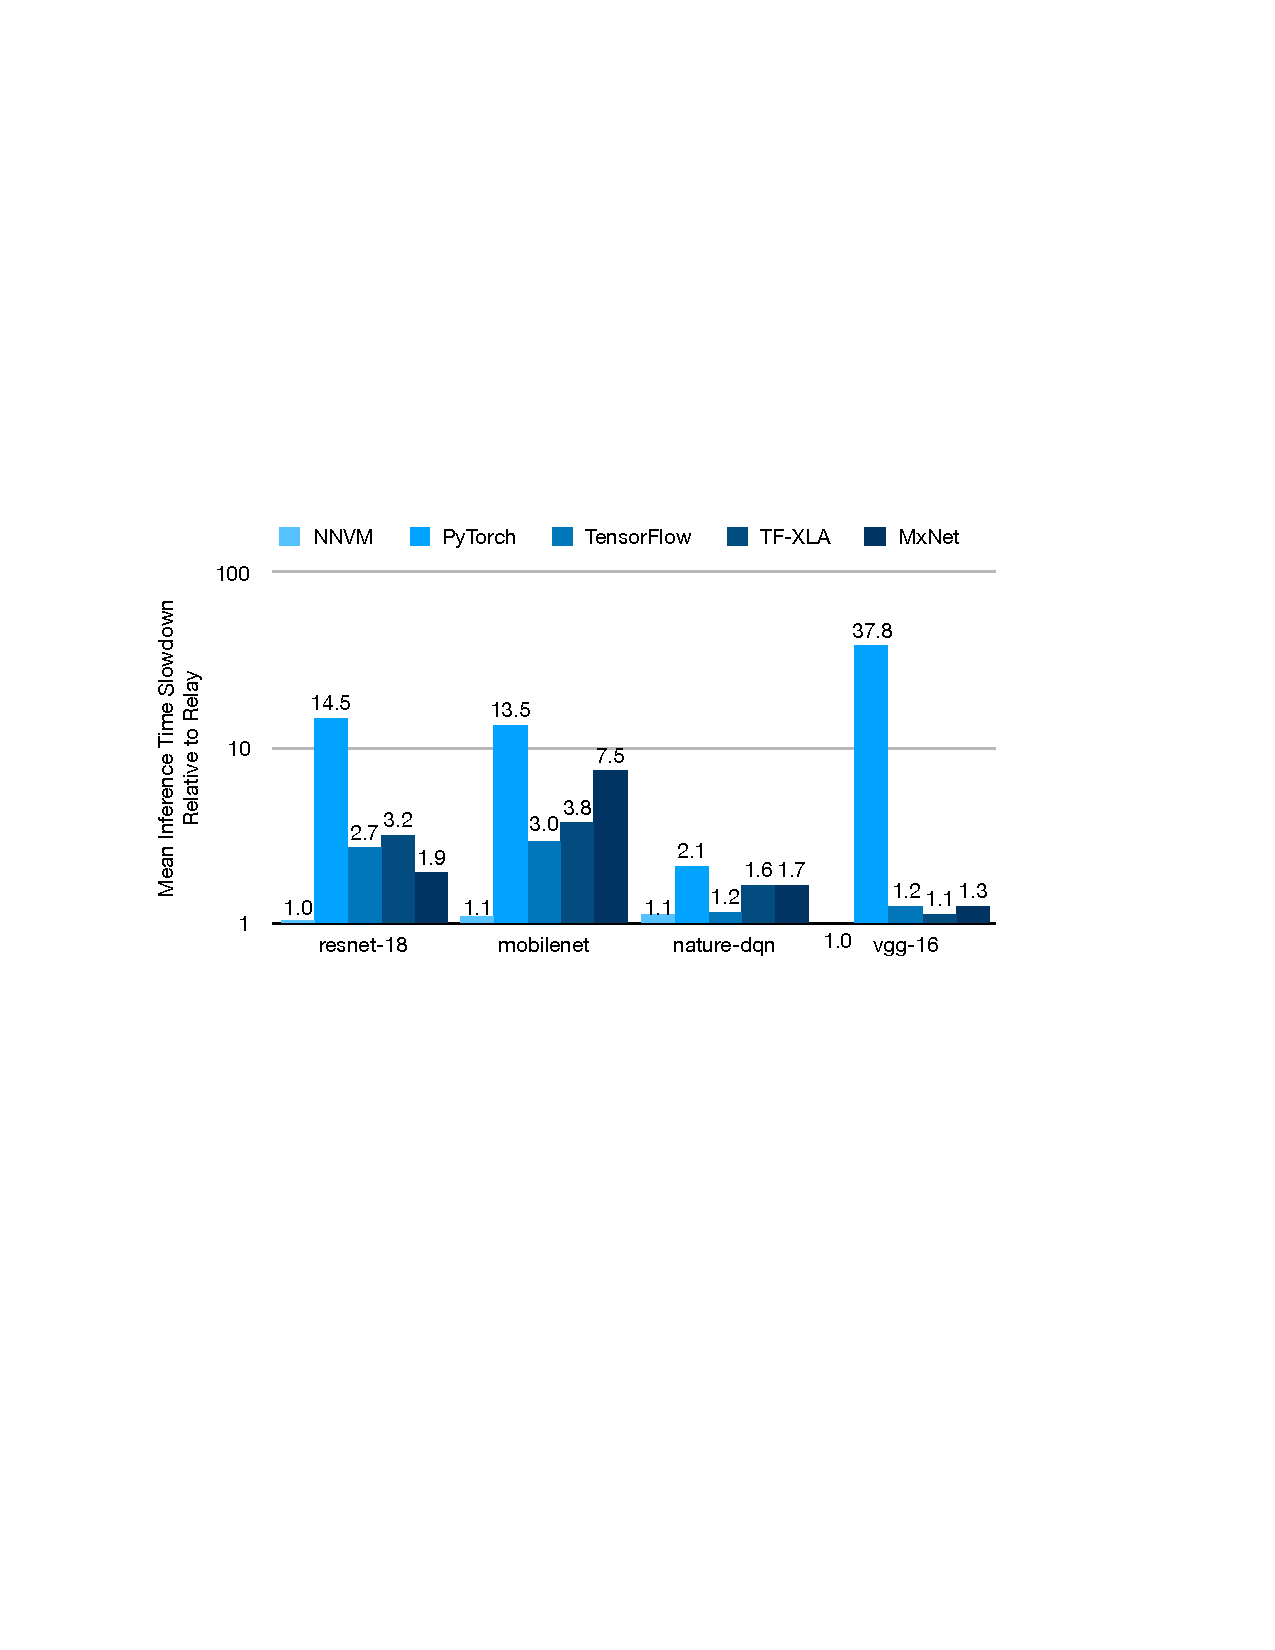
\includegraphics[width=
    \textwidth]{fig_splash19/eval/vision_1080Ti_relay.pdf}
    \caption{
      Inference slowdown of popular frameworks relative to Relay on vision
        benchmarks running on NVIDIA GTX 1080 Ti GPUs.
      Relay provides performance competitive to the state of the art.
      We ran 1000 trials for each model and used the AoT compiler.
    }
    \label{fig:vision-eval}
  \end{figure}

  \begin{figure}[h]
    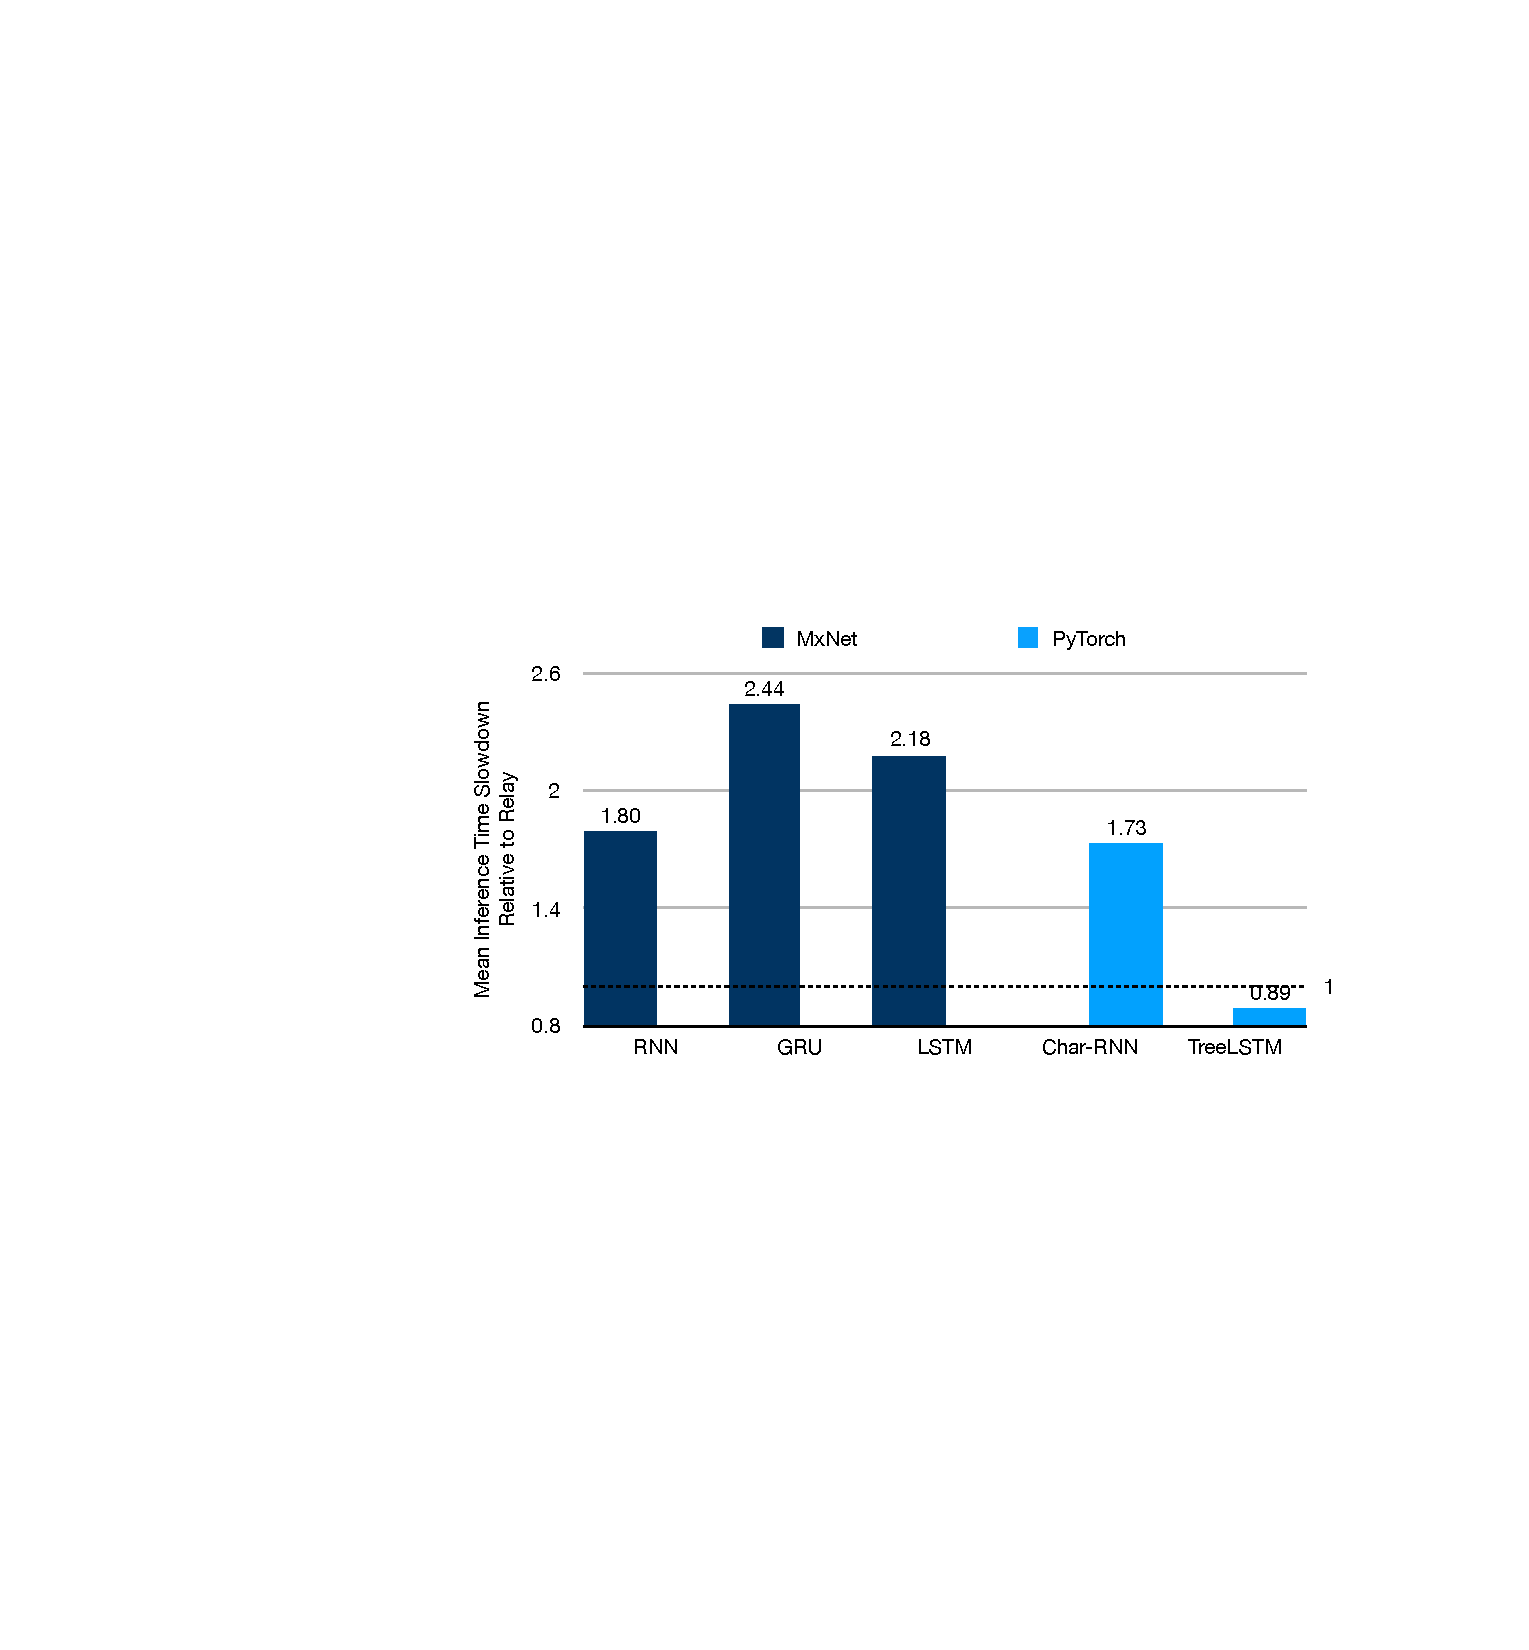
\includegraphics[width=
    \textwidth]{fig_splash19/eval/nlp_TitanV_relay.pdf}
    \caption{
      Inference slowdown relative to Relay on NLP benchmarks running on NVIDIA
        Titan-V GPUs.
      NLP workloads feature control flow,
        which makes them more challenging to optimize.
      Relay provides performance competitive to state of the art (up to
        2.4$\times$ speedup over MxNet on GRU).
      We ran 1000 trials for each model, except for CharRNN, on which we used 100 trials.
    }
    \label{fig:nlp-eval}
  \end{figure}

  An age-old story in compilers literature is that increasing expressivity
    impacts the global performance of the system.
  We set out to build zero-cost abstractions for Relay,
    governed by Stroustrup's principle, ``What you don't use, you don't pay
    for'' \citep{bjarne}.
  We demonstrate that we can achieve competitive performance on both CPUs and
    GPUs on a wide set of CNNs that are well supported by existing frameworks.
  We evaluated inference time for two classes of workloads: computer vision and natural language processing.
  We compared Relay (using our AoT compiler) to \nnvm,
    TensorFlow, TensorFlow-XLA (Accelerated Linear Algebra), PyTorch, and MxNet.
  We ran the vision and NLP workloads on GTX 1080 Ti and Titan-V GPUs, respectively.

  \subsection{Vision Evaluation}
  % Figure~\ref{fig:vision-eval} compares Relay against state of the art frameworks
  %   running vision workloads on a GTX 1080 Ti GPU.
  We ran each model with
    batch size 1, a common setting in inference tasks.
  Relay achieves performance on par with \nnvm,
    an existing deep learning graph compiler in use at Amazon.
  Relay outperforms TensorFlow, TensorFlow-XLA, MxNet and
    PyTorch on every benchmark.
  Relay's ability to do aggressive optimizations like operator
    fusion on long chains of operations, generating hardware
    specific implementations, enables it to outperform
    existing frameworks that don't perform inter-operator optimizations.

  \subsection{NLP Evaluation}
  % Figure~\ref{fig:vision-eval} compares Relay against state-of-the-art NLP models on a Titan-V GPU.
  % Implementations of the NLP models were not available in all frameworks;
    we used MxNet baselines for RNN, GRU, and LSTM and PyTorch for Char-RNN and TreeLSTM.
  % We ran the models for 1000 iterations per input, except char-RNN, which we ran for 100 ???.
  % To run the RNN, GRU, and LSTM benchmarks in MxNet, and Char-RNN, and TreeLSTM
  %   in PyTorch.
  Relay performs better than MxNet on recursive models
    due to the fact they are implemented in Python using
    MxNet's looping constructs.
  PyTorch instead uses handwritten and heavily optimized
    C implementations of the recursive network cells.
  Due to this we perform slightly \emph{worse} than PyTorch.
  It is interesting to note that our pure Relay
    implementation performs competitively against
    the hand-optimized version.

  \subsection{Targeting Deep Learning Accelerators on FPGAs}

  \begin{figure}[h]
    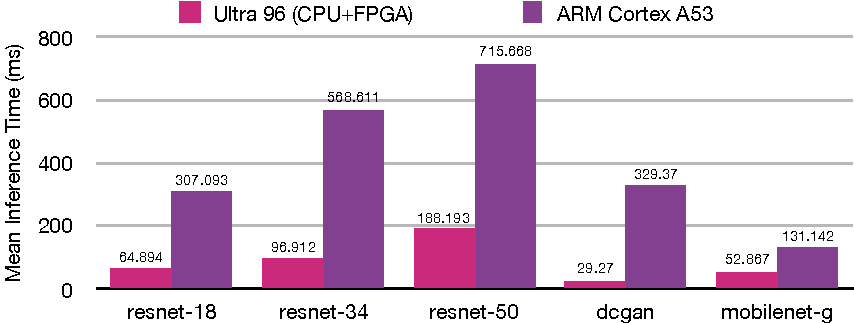
\includegraphics[width=\textwidth]{fig_splash19/eval/vision_fpga.pdf}
    \caption{
      Inference time (ms) of vision DNNs on Ultra-96 FPGA-enabled SoC.
      We compare vision workloads that Relay compiles onto the embedded Cortex
        A53 CPU vs. a DNN accelerator implemented on the integrated FPGA fabric.
      Targeting DNN accelerators can unlock up to 11x speedups, but requires a
        multitude of graph-level transformations.
      We used 10 trials for each model.
    }
    % \label{fig:fpga-eval}
  \end{figure}

  We evaluated inference time on five models including MobileNet-G \citep{mobilenet}, a grouped variant of the MobileNet architecture; ResNet-18, ResNet-34, and ResNet-50\citep{resnet}; and Deep Convolutional Generative Adversarial Networks \citep{dcgan}, a generative DNN used in unsupervised learning.
  Overall, Relay helps us efficiently offload deep learning operators onto specialized accelerators like VTA.
  Our results in Figure~\ref{fig:fpga-eval} show that we can achieve between 2.5 to 11.7$\times$ reduction in single-batch inference latency by offloading critical operators to the FPGA accelerator.
  These experiments demonstrate Relay's ability to target current and future deep learning architectures:
  \begin{enumerate}
    \item \textit{Heterogeneous FPGA/CPU offloading}: Relay lets us define the rules for offloading specific operators to the FPGA-based accelerator.
    \item \textit{Push-button quantization}: Relay can take a \texttt{fp32} model and convert its parameters to \texttt{int8} in order to enable inference on specialized accelerators.
    \item \textit{Accelerator-friendly data packing:} Relay reorganizes data so it can be effortlessly consumed by a specialized TPU-like accelerator~\citep{tpuv1}.
  \end{enumerate}

The scenario presented in the introduction demonstrates the three-pronged \textbf{extensibility challenge}
  for DL IRs:
% \begin{enumerate} % [label=\arabic*.]
%   \item \textit{Expressivity}: It should be straightforward to write models involving complex data structures (e.g., trees, graphs, and lists) and control flow.
%   \item \textit{Composability}: It should be straightforward to add and compose new optimizations
%     with existing ones (e.g., quantization, operator fusion, and automatic differentiation).
%   \item \textit{Portability}: It should be straightforward to add new hardware backends
%     (e.g., TPU, Inferentia, and FPGAs)~\citep{tpuv1, inferentia}.
% \end{enumerate}


% Differentiation
% Core is AD + PE
\chapter{Automatic Differentiation}
\label{ch:ad}

In deep learning merely specifying tensor computations is
  one only one piece of the puzzle, as one must be able
  differentiate networks in order to perform optimization.
Many popular optimization algorithms,
  such as stochastic gradient descent
  rely on the ability to take
  the gradient (directional derivative) of the function with
  respect to some parameters.
Early frameworks provided heavily structured optimization frameworks
  which directly implemented the backpropagation algorithm for training
  deep neural networks.
The backpropagation algorithm combines
  computing the gradient of a loss function defined over the
  output of a network with respect to some parameters, and an
  optimization step which updates each parameter based on its
  gradient.
Modern deep learning frameworks have realized that the
  structured imposed by backpropagation is not fundamental
  and model definitions can be expressed more uniformly.
For example we can break down a deep neural network training
  process into (1) a network definition, a function defined over tensor inputs,
  (2) a loss function, which computes a scalar score from tensor
  inputs, and (3) an update step which modifies each of the parameters using their gra
  gradient with respect to the loss function.
All of these pieces can be written as programs which manipulate tensors,
  except for the gradient which requires transforming
  one computation into another which computes its directional derivative.

Early systems such as Theano demonstrated that automatic
  differentiation, the process of automatically computing gradients,
  accelerates research in machine learning by removing the need to manually
  derive gradients.
There are many ways to approximate or compute the gradient of a function
  but automatic differentiation is favored due to its precise gradient
  values and runtime efficiency.
Early automatic differentiation work made use of runtime data structures
  which store a trace of all operations invoked and computes the gradient
  dynamically by just applying chain rule.
This approach is very flexible as it allows users to implement a small number
  of primitive gradients and handle a large variety of programs which combine
  these primitives.
Unfortunately this purely runtime based approach means that even if a program
  is known a priori we must dynamically construct and execute its gradient.
The dynamic nature induces both static overhead, but also limits ahead of time
  optimization, or deployment to resource limited devices.

In order to address these weaknesses many have reformulated
  automatic differentiation as a source code transformation
  where AD transforms a function into one which computes its gradient.
The generated gradient function is just a standard tensor programming
  enabling uniform optimization and compilation.
This approach has enjoyed recent popularity due its conceptual
  elegance and uniformity.
For example a quantization technique defined as a program
  transform can then be applied to the forward and backward passes
  of your network without needing a special version of quantized AD.
Unfortunately these source code transformations do not cleanly
  generalize to all language features or dynamic behaviors such
  as closures, mutation, control-flow, data structures or dynamic allocations.
There have been numerous previous approaches attempting to handle a large number
  of features as described in Chapter~\ref{ch:related}.
The rest of this chapter explores how to build on the simplicity of
  tape-based AD, by adapting it higher-order imperative languages,
  resulting in a source code transformation which supports dynamic features
  without giving up the ability to compile and optimize.
We close the chapter focusing on how partial evaluation is essential to this
  approach.

\subsection{Automatic-Differentiation}

As discussed in Chapter~\ref{ch:related} Automatic Differentiation has a long history
  and numerous applications across many fields.
The style of automatic differentiation popular when we began this work was the
  what is known as a Wengert-list, a runtime data structure which tracks
  all operations performed, as well as its inputs and outputs, recording them on tape
  that can be later replayed to compute the partial derivative with respect to each variable.
Approaching automatic differentiation in this style leads to a relatively simple
  implementation which can handle arbitrary language features.
When performing differentiation we need not consider data
  structures, control, scope, or any other language features as they
  have been computed away.
We only see a trace of operations of unrolled in time, allowing us
  to simply apply the chain rule from basic calculus.
This approach is beautifully simple as we do not need to formulate
  clever ways to account for each language feature.
Unfortunately the dynamic nature of this solution requires tracking extra runtime state
  and performing computation for each operation, as well as providing an incomplete
  view on the computation which often limits available optimizations.

A design goal of Relay is to provide a target agnostic substrate on which
  to build more complex compilers.
When starting to work on training and automatic differentiation we had
  the same design goal, we wanted to enable training frameworks which
  could use a single code base to provide state-of-the-art performance
  without compromising expressivity.
For example train a model on a cloud GPU or a micro-controller without
  needing to change your workflow.
Exploring training demanded an automatic differentiation method that can
  execute in multiple execution environments while handling Relay's increased
  expressivity.
We can work backwards from our requirements to eliminate some courses
  of action.
We need an algorithm which handles Relay's dynamic features, maintains
  key properties such as static typing, enables ahead of time optimization,
  and be compiled through standard flows.
During the period we did this work there were numerous
  groups working on variations of this problem for numerous systems
  as detailed in Chapter~\ref{ch:related}.
We ruled out existing approaches
  as many of them violated our requirements, some required dynamic typing
  and/or reflection, others required complex AD rules per language feature,
  were only defined on SSA, or used staging to remove features not supported
  by less expressive IRs.
After many iterations we discovered a design which uniquely achieved these
  three goals with relative simplicity:
\begin{itemize}
  \item Handles all language features including closures,
        references, control flow, and data structures.
  \item Maintains static typing of programs, and by extension shape inference.
  \item Can be performed as an ahead of time source code
    transformation allowing program to be uniformly optimized.
\end{itemize}

% Relay requires an algorithm that operates as a source code transformation
%   and supports higher-order functions and higher-order gradients.
% There is a large body of work on performing AD
%   of programs.
% Several full-length papers have been written about automatic
%   differentiation (AD).
% This section highlights the important differences
%   between our approach and other recent work.
% Previous approaches like Lantern~\citep{lantern} (see Chapter~\ref{ch:related})
%   define a generic and powerful version of AD.
% Lantern uses delimited continuations to implement AD.
% Delimited continuations are an elegant solution
%   but require language and compiler support,
%   as well garbage collection.
% Furthermore, delimited continuations are challenging
%   to reason about when performing optimization.

\subsection{Higher-Order, Higher-Order Automatic Differentiation}
\label{sec:autodiff}

Previous automatic differentiation (AD) techniques used on
  computation graphs cannot be directly applied to Relay due to new
  language features such as closures, recursion, and control flow.
Furthermore, it is becoming increasingly important to compute not
  only first-order gradients of functions
  but potentially $n$th-order gradients~\citep{neural_ode, darts}.
These two challenges were our original motivation to pursue
  a new automatic differentiation technique.
Our AD algorithm is conceptually a source code transformation
  version of the Wengert List or tape-based method of AD.
We make a few core changes.
First, our algorithm is defined as a source code
  transformation.
Given an expression, Relay produces a corresponding
  expression that computes its gradient.
Figure \ref{fig:autodiff_rules} provides a denotation from
  Relay expression to Relay expression that defines our
  AD algorithm.
Second, our algorithm eschews ideas such as delimited continuations
  in favor of an approach using closures and references.
Relay simply pairs all tensor values with a reference
  that tracks its partial derivative with respect to its
  output.
This form of reverse mode AD is similar to how one
  would implement forward mode AD.
Relay lifts all tensor-typed values to a pair,
  an expression of some tensor type \verb|T| becomes a tuple of \verb|(T, Ref<T>)|
  where the second component contains the sensitivity variable
  needed to compute the partial derivative.
For each gradient function generated, Relay allocates
  a single reference which stores the ``backpropagator,''
  a closure which propagates gradients from the output to the input.
Each subcomputation affecting the gradient updates this closure; when it is
  finally executed, the built-up closure returns the final derivatives with respect to
  to the arguments.

As described in Figure~\ref{fig:autodiff_rules}, only
  computations involving tensors contribute to the gradient.
For example, we support mutability for free because mutation
  does not affect the gradients.
In this sense, our design is simple.
All tracing needed to compute derivatives is done at run time, enabling
  support for higher order functions, higher order gradients,
  data-dependent control flow, and mutability without requiring changes
  to the algorithm.
Finally, Relay exposes this transformation as an operator, allowing users
  to compute the gradient of a function \verb|f| simply by writing \verb|grad(f)|.

Many other variants of AD, including algorithms with different
  complexity bounds (e.g., forward-mode AD), exist.
Forward-mode AD is useful for computing the
  Hessian vector product, which is necessary for techniques like differentiable architecture search
  (DARTS)~\citep{darts}.
Because our AD algorithm just another Relay pass,
  it is possible for users to implement and experiment with different
  AD techniques without changing the system.
To this end, we also implemented a  forward-mode AD algorithm using the traditional method of dual
  numbers~\citep{ad_survey}.
Both forward-mode and reverse-mode AD are higher-order and extensible: they
  support closures, abstract data types, control flow, and recursion.
Although we have not investigated
  composing forward and reverse modes,
  it is possible to mix gradient functions
  because they are regular Relay functions.
Because our algorithm enjoys a closure property,
  we can perform AD over the composition of the gradient
  functions.

\begin{figure}
    % NOTE: We need to explain that `\revv{f}' is the registere gradient of `f'.
    \centering
    $\begin{array}{lll}
      % Tensor Type
      \textsf{ADType}\left(\kwd{Tensor } t\right) &=& \rTuple{t}{\kwd{Ref[}t\kwd{]}} \\[0.5em]
      % Tuple Type
      \textsf{ADType}\left(\rTuple{t_0}{\cdots}{t_n}\right) &=& \rTuple{\textsf{ADType}(t_0)}{\cdots}{\textsf{ADType}(t_n)} \\[0.5em]
      % Variable
      \textsf{ADTerm}\left(\kwd{Var } x\right) &=& x \\[0.5em]
      % Reference
      \textsf{ADTerm}\left(\kwd{Ref } e\right) &=& \kwd{ref(}\textsf{ADTerm}(e)\kwd{)} \\[0.5em]
      % Literal
      \textsf{ADTerm}\left(\kwd{Lit } l\right) &=& \rTuple{l}{\kwd{ref(}\texttt{0}\kwd{)}} \\[0.5em]
      % Tuple
      \textsf{ADTerm}\left(\rTuple{e_0}{\cdots}{e_n}\right) &=& \rTuple{\textsf{ADTerm}(e_0)}{\cdots}{\textsf{ADTerm}(e_n)} \\[0.5em]
      % Match
      \textsf{ADTerm}(\kwd{match (} e\kwd{) \textbraceleft} &=& \kwd{match (}\textsf{ADTerm}(e)\kwd{)} \kwd{ \textbraceleft} \\
      \quad \kwd{| } p_0 \rightarrow e_0 & & \quad \kwd{| } p_0 \kwd{ $\rightarrow$ } \textsf{ADTerm}(e_0) \\
      \quad \vdots & & \quad \vdots \\
      \quad \kwd{| } p_n \rightarrow e_n & & \quad \kwd{| } p_n \kwd{ $\rightarrow$ } \textsf{ADTerm}(e_n)\\
      \kwd{\textbraceright}) & & \kwd{\textbraceright}
      \\[0.5em]
      % Function
      \textsf{ADTerm}(\kwd{fn (} &=& \kwd{fn (} \\
      \quad \rParam{x_0}{t_0}\kwd{,} & & \quad \rParam{x_0}{\textsf{ADType}(t_0)}\kwd{,} \\
      \quad \vdots\kwd{,} & & \quad \vdots\kwd{,} \\
      \quad \rParam{x_n}{t_n} \kwd{)} & & \quad \rParam{x_n}{\textsf{ADType}(t_n)} \kwd{)} \\
      \quad \quad \kwd{$\rightarrow$ } t_{\text{ret}} & & \quad \kwd{$\rightarrow$ } \textsf{ADType}(t_{\text{ret}}) \\
      \kwd{\textbraceleft }\,\,\, e \kwd{ \textbraceright}) & & \kwd{\textbraceleft }\,\,\, \textsf{ADTerm}(e) \kwd{ \textbraceright}\\
      \\[0.5em]
    % \end{array}$
    % $\begin{array}{l}
      % Call
      \textsf{ADTerm}\left(f\rTuple{e_0}{\cdots}{e_n}\right) \ \ \  = \\
      \quad \rLet{\revv{e_0}}{}{\textsf{ADTerm($e_0$)}}{} \\
      \quad \vdots \\
      \quad \rLet{\revv{e_n}}{}{\textsf{ADTerm($e_n$)}}{} \\
      \quad \rLet{v}{}{f\rTuple{\revv{e_0}\kwd{.}\texttt{0}}{\cdots}{\revv{e_n}\kwd{.}\texttt{0}}}{} \\
      \quad \rLet{\bper{v}}{}{\kwd{ref(}\texttt{0}\kwd{)}}{} \\
      \quad \kwd{let } \delta \kwd{ = fn () \textbraceleft} \\
      \quad \quad \rLet{\rTuple{\sens{e_0}}{\cdots}{\sens{e_n}}}{}{\\ \quad \quad \quad \revv{f}\rTuple{v}{\kwd{!}\bper{v}}{\kwd{!}\revv{e_0}\kwd{.}\texttt{0}}{\cdots}{\kwd{!}\revv{e_n}\kwd{.}\texttt{0}}}{} \\
      \quad \quad \revv{e_0}\kwd{.}\texttt{1} \kwd{ $\pluseq$ } \sens{e_0} \kwd{;} \\
      \quad \quad \vdots \\
      \quad \quad \revv{e_n}\kwd{.}\texttt{1} \kwd{ $\pluseq$ } \sens{e_n} \kwd{;} \\
      \quad \quad \kwd{()} \\
      \quad \kwd{\textbraceright;} \\
      \quad \Delta \kwd{ $\coloneqq$ } \kwd{!}\Delta \kwd{ $\circ$ } \delta \kwd{;} \\
  %    \quad \Delta \kwd{ := } \kwd{!}\Delta \kwd{ $\circ$ } \delta \kwd{;} \\
      \quad \rTuple{v}{\bper{v}}
    \end{array}$
    \caption{
      Transformation Rules for Automatic Differentiation in Relay.
      The most interesting case is for function calls.
      The backpropagator $\Delta$ is initialized to \kwd{ref(fn() \textbraceleft\ ()
        \textbraceright)} at the top level of each \textsf{ADTerm} call.
      Successive update closures $\delta$ are then composed with $\Delta$ to
        form a chain.
      Syntactic sugar is used for some constructs which are not available as
        primitives in Relay.
    }
    \label{fig:autodiff_rules}
  \end{figure}


\subsection{Partial Evaluator}
\label{sec:partial_eval}

\begin{figure}
  \centering
  % \texttt{\bf Identity Function}
  \judgbox{\texttt{\bf Identity Function}}{}
    \begin{minted}{rust}
fn <s, bt>(%d: Tensor[s, bt]) {
  %d
}
    \end{minted}

  \judgbox{\texttt{\bf Post-AD}}{}

    \begin{minted}{rust}
fn <s, bt>(%d: Tensor[s, bt]) {
  let %x = ref(fn () { () });
  let %x1 = (%d, ref(zeros_like(%d)));
  let %x2 =
    (fn <s, bt>(
      %d1: (Tensor[s, bt],
            ref(Tensor[s, bt]))) {
      %d1
    })(%x1);
  %x2.1 := ones_like(%x2.0);
  let %x3 = read(%x)();
  (%x2.0, (read(%x1.1),))
}
    \end{minted}
  \judgbox{\texttt{\bf Post-PE}}{}

    \begin{minted}{rust}
fn <s, bt>(%d: Tensor[s, bt]) {
  let %x = fn () {
    let %x1 = ();
    %x1
  };
  let %x2 = ref(%x);
  let %x3 = zeros_like(%d);
  let %x4 = ref(%x3);
  let %x5 = (%d, %x4);
  let %x6 =
    fn <s, bt>(
      %d1: (Tensor[s, bt],
            ref(Tensor[s, bt]))) {
      %d1
    };
  let %x7 = ones_like(%d);
  %x4 := %x7;
  let %x8 = ();
  let %x9 = (%x7,);
  let %x10 = (%d, %x9);
  %x10
}
    \end{minted}

  \judgbox{\texttt{\bf Post-DCE}}{}

    \begin{minted}{rust}
fn <s, bt>(%d: Tensor[s, bt]) {
  (%d, (ones_like(%d),))
}
  \end{minted}
  \caption{
    Example of running the compiler pass pipeline for AD on the identity
    function.
    First, we run the base AD pass on the original function (described in Section \ref{sec:autodiff}).
    Then, we run the partial evaluator,
      which primarily optimizes away the reads and calls in \texttt{\%x2} and
      \texttt{\%x3} in post-AD.
    Since it conservatively determines whether a subexpression is effectful,
      it generates many bindings which are dead code.
    At this point, we run the dead code elimination pass to crunch the code back down.
  }
  \label{fig:pe-example}
\end{figure}



Existing deep learning IRs have relied on
  a mixture of staging and constant evaluation
  in order to optimize user programs.
Partial evaluation is a generalized form of constant
  evaluation that can reduce partially constant
  programs.
A partial evaluator (PE) allows the use of high-level abstractions
  without limiting code that \textit{could} in practice be
  compiled to a particular target.
Relay is the first compiler to apply partial evaluation
  techniques to deep learning, the
  core approach of which is based on \citep{pe_ref}.
Partial evaluation, when composed with other
  optimizations like fusion, yields a variety
  of useful optimizations without requiring
  a separate implementation of each.
For example, the partial evaluator can be used to perform
  loop unrolling, which then enables further fusion,
  without any additional compiler passes.

Existing deep learning IRs have relied on
  a mixture of staging and constant evaluation
  in order to optimize user programs.
Partial evaluation is a generalized form of constant
  evaluation that can reduce partially constant
  programs.
A partial evaluator (PE) allows the use of high-level abstractions
  without limiting code that \textit{could} in practice be
  compiled to a particular target.
Relay is the first compiler to apply partial evaluation
  techniques to deep learning, the
  core approach of which is based on \citep{pe_ref}.
Partial evaluation, when composed with other
  optimizations like fusion, yields a variety
  of useful optimizations without requiring
  a separate implementation of each.
For example, the partial evaluator can be used to perform
  loop unrolling, which then enables further fusion,
  without any additional compiler passes.

In order to handle differentiating the full IR,
  our AD algorithm makes use of closures and references.
However many of the programs are effectively
  first-order and do not require allocating
  references or a backpropagator closure.
It is essential we remove unnecessary uses
  of closures and references as they inhibit
  optimizations like operator fusion.
Previous approaches have used staging to manually
  phase computation, but this requires modifications
  to the language itself.
A partial evaluator (PE) allows the use of high-level abstractions
  without limiting code that \textit{could} in practice be
  compiled to a particular target.
The benefits of partial evaluation do not only extend to code
  generated by AD but for all of Relay.
Relay's partial evaluator works by defining a interpreter
  where the value domain is partially static values.
The partially static domain represents simple values,
  such as constant tensors, as themselves. The representations
  of aggregate values mirror their structure, enabling
  values which are a mixture of static and dynamic.
This makes the partial evaluator more powerful
  than a constant-folding pass.
The appendix presents an implementation of PE.

There are two important features of our partial evaluator:
  managing effectful computations and handling references.
In order to handle effects, we keep the generated
  program in A-normal form to ensure effects are properly ordered
  and to avoid the duplication of effectful computations.
The partial evaluator supports references by
  simulating the store at partial evaluation time.
The explicit store is threaded throughout execution
  and is managed to achieve flow sensitivity.
After evaluation we construct a new program with
  static subcomputations evaluated
  away.
The reconstructed program contains all original
  expressions, as well as evaluated expressions,
  because interleaving dead-code elimination (DCE) is
  non-trivial.
Afterwards, we separately apply DCE.
The result of this entire process is illustrated
  in Figure~\ref{fig:pe-example}.

  Relay's partial evaluator works by defining a interpreter
  where the value domain is partially static values.
The partially static domain represents simple values,
  such as constant tensors, as themselves.
The representations
  of aggregate values mirror their structure; for example,
  tuples become a tuple of partially static values.
The partially static domain represents dynamic values,
  which may not be known until execution time,
  alongside the static values traditionally supported by
  constant evaluators.
Our partial evaluator must solve two important problems:
  managing effectful computations and handling references.
In order to handle effects, the evaluator keeps the generated
  program in A-normal form to ensure effects are properly ordered
  and restrict duplication of effectful computations.
The partial evaluator supports references by
  simulating the store at partial evaluation time.
The explicit store is threaded throughout execution
  and provides a flow-sensitive PE.
Finally, the evaluator constructs a new program with
  the static subcomputations evaluated away.
% The reconstructed program contains all original
%   expressions, as well as evaluated expressions,
%   because interleaving dead-code elimination (DCE) is
%   non-trivial.
% Afterwards, we separately apply DCE.
% The partial evaluator has use cases beyond inference
%   optimizations, separately it enabled the design of an automatic
%   differentiation algorithm that makes use of hard to optimize
%   features such as references of closures, as the partial evaluator
%   can remove unneeded abstraction.

% \chapter{ML Frameworks}
\label{ch:frameworks}

Using Relay as a building block for ML frameworks.


\subsection{Beacon}

A related challenge is increasing the ability for users to describe models which take
  full advantage of \relay's more expressive semantics.
As discussed in \ref{ch:related} existing frontends have been designed to capture the
  subset of programs which be optimized well, and designs have ignored aspects of the
  programs that are not well optimized.
In order to demonstrate what we can do with greater access to the program we constructed
  Beacon a PyTorch-like inspired framework which uses TVM for all execution.

Beacon uses a novel design related to ideas from previous work detailed in \ref{ch:related}
  in order to convert Python directly into IR which can be compiled by \relay.
Beacon simply defines a tensor which stores either a value or a partial program
  which can be used to execute the program.
Beacon's core abstraction can be summarized in a small fragment of code, seen below.

\begin{figure}
\begin{minted}{python}
  class Tensor:
    def __init__(self, expr, value=None):
        self.expr = expr
        self._value = value

    def value(self, evaluator="debug"):
        mod = get_module()
        ex = relay.create_executor(kind=evaluator, mod=mod)
        inputs = relay.ir_pass.free_vars(self.expr)
        binds = dict((var, _lookup_var(var)._value) for var in inputs)
        return ex.evaluate(self.expr, binds).data
\end{minted}
\end{figure}

Because Beacon serves as a thin abstraction on top of Relay it
  is easy to try out new approaches for generating IR, and build
  higher level abstractions, such as iterators which construct
  loopy IR, or using program rewriting techniques like those
  used in AutoGraph~\citep{AutoGraph}.
Users can also use pure Python to construct arbitrary Relay
  programs which can then be ahead of time optimized and
  deployed.
Beacon serves as a platform for experimenting with how
  to use the IR, and inform optimizations and accelerator optimizations.
Beacon is just a starting point, we will discuss how to enable this for frameworks
  such as PyTorch and MxNet in Section \ref{sec:future}.

% Optimizations
% Core is Opts.
\chapter{Optimizations}
\label{ch:optimizations}

Building a compiler can be likened to building a bridge between
    two distant points.
The semantic gap between your starting point and end point imply the
    complexity of the structure needed to bridge the gap.
Optimizations are the building blocks of such a structure.
If one chooses an input representation sufficiently close to
    the target representation compilation is relatively straight forward
    and often little to no optimization is needed.
Unfortunately as the semantic gap and complexity are inextricably linked
    and as it grows so does the difficulty of writing effective optimizations.
It is not sufficient for a compiler author to be able to perform an
    optimization by hand but they must be able to generalize it into
    a repeatable, inductive process.
The challenge introduced by using a sufficiently abstract and high-level
    representation is designing the transformations and optimizations
    to get us to our end goal.
Given that our goal is state-of-the-art performance in competitive
    area, it is critical we get our optimizations right.
Over the course of my PhD thesis we have designed more than 50 passes
    for Relay, enabling TVM to reach state-of-the-art performance
    on numerous real world models~\citep{huggingface_octoml}.
This chapter focuses on the design and implementation of selected passes.
The remainder of which exist in Apache TVM's source tree
  and are open to all to read and inspect.

\section{Operator Fusion}
\label{sec:fusion}

Operator fusion is an indispensable optimization in deep learning compilers.
Fusion enables better sharing of computation, removal of
  intermediate allocations, and facilitates further optimization by
  combining loop nests.
Fusion is known to be the most critical optimization in machine
  learning compilers, but existing fusion techniques
  are closed (working over a fixed set of ops)
  and target-dependent.
Traditional operator fusion algorithms resemble instruction
  selection:
A sequence of operators eligible
  for fusion is first identified and then replaced with a corresponding
  handwritten fused implementation, usually from a vendor-provided library.
For example, if a fused implementation for a GPU operator does not exist in CuDNN,
  it will remain unfused.
More advanced strategies, implemented in XLA, detect a
  closed set of statically shaped operators for fusion and
  generate code for CPU/GPU.

Relay's fusion algorithm addresses weaknesses of previous approaches by representing
  \textit{all} operators in a secondary IR.
Relay operators are backed by a TVM compute expression that
  describes operations in a high-level DSL that resembles Einstein notation
  but omits low-level scheduling details.
TVM's separation of compute and scheduling provides many favorable qualities
  for Relay's fusion algorithm.
It enables producing shape-specialized fused operators for an open set of operators,
  fusing arbitrary-length chains of operators (not just pairwise combinations),
  and handling operators with multiple outputs and nonlinear consumer-producer patterns.
TVM is also able to reschedule after fusion and perform further optimization via auto-tuning.
Relay performs fusion in two steps, detailed below.

\section{Extraction}

First, Relay identifies subexpressions containing
  fusion-eligible and factors them into local functions that
  are marked as primitive.
Primitive functions can later be lowered to platform-specific
  code.
Fusion-eligible subexpressions are identified by constructing a
  directed acyclic graph (DAG) representing data flow between operators.
As the dataflow DAG is acyclic, it allows for the simple construction
  of a post-dominator tree.
Subexpressions are grouped into equivalence classes
  determined by their immediate post-dominator.
The use of the post-dominator tree enables fusion
  between non-linear producer-consumer relationships;
  for example, Relay can fuse diamond-shaped data-flow relations,
  where an input is used by multiple parallel operator chains
  that are combined again by a later operator.
Finally, Relay constructs an expression from each equivalence class,
  collects the expressions' free variables,
  constructs a function with the expression as the body and the free variables
  as parameters,
  and marks it as primitive.

\section{Lowering}

In a second step, the Relay compiler converts the generated primitive
  function into platform and shape specific code.
For each operator, Relay collects the high-level \tvm expression that represents it,
  then combines them into an aggregate expression that represents the fused operation.
Generating code using \tvm also requires producing a schedule.
It is possible to use \tvm's default schedule to generate code for a single operation,
  but the default schedule does not support fusion.
In order to generate code for the combined expression, we must generate a
  master schedule based on the set of operations being fused.
The fusion algorithm analyzes the expressions to select a master
  schedule, the master schedule will perform the appropriate scheduling
  actions to generate fused code, such as inlining loops, or reorganizing
  computation.
By combining the master schedule with the fused computation,
  Relay is able to produce an optimized version of the operator
  for any platform supported by TVM.
For example, a related project by one of the co-authors implemented
  a RISC-V backend which immediately obtained full operator fusion
  with no new code.
Due to the Relay compiler's integration with AutoTVM, we can further
  optimize fused operations by performing auto-tuning on the master
  schedule template to obtain the best performance.

\section{Generic Quantization Framework}
\label{sec:quant}

Deep learning is constrained by memory, compute, and accuracy.
Accuracy is often the only metric optimized by machine learning
  researchers, leading to compute- and memory-hungry models.
The sheer number of parameters and the requisite compute
  makes deploying models to resource-limited devices,
  such as in mobile or IoT, challenging.
Even in non-edge devices, the compute cost of using
  datatypes like FP32 is large and computing with mixed precision
  or reduced precision can aid performance.
 An emerging area in deep learning is performing training and inference on
  non-standard numeric types to improve throughput and memory usage.
For example, a single neural network may have more than one million floating-point values
  as its parameters.
The sheer quantity of parameters and their datatypes may limit the ability
  to execute these networks on hardware accelerators.
Accelerators often support fixed point or other non-standard datatypes, at lower precision.
In order to target these devices, Relay must map the computation
  to the appropriate domain.
Unfortunately, reducing bit-width is not a silver bullet and
  can dramatically harm model accuracy.
The tradeoffs between these quantities has lead to the study of quantized neural networks,
  the process by which NNs are modified to use a smaller precision
  or non-standard datatypes to improve throughput and memory usage.
Quantization is particularly essential for supporting many accelerators due to
  their restricted set of datatypes.

State-of-the-art work on quantization suggests that there exist a number of tradeoffs
  between different quantization techniques,
  with the best often determined by platform and model type~\citep{krishnamoorthi18}.
Current deep learning frameworks support a limited number of quantization schemes, and options
  because quantization requires framework support in the form of custom platform-specific operators.
Importantly, there are many different choices of quantization mechanisms.
Each type of quantization has different running time and accuracy properties depending
  on the model as well as the target hardware.
Existing frameworks manually choose a fixed quantized data format, which might be
  suboptimal.
Instead, Relay includes a generic, compiler-based quantization flow that supports a diverse set
  of quantization mechanisms and automatically generate code for each of them.
Relay's generalizable and flexible quantization workflow
  can support customization in both standard devices and acceleration schema
  and address various constraints across different hardware platforms.
The pipeline that we designed can compress and accelerate neural networks with
  low-precision quantization to enable running the deep learning models on edge devices.
Users can overload Relay's existing quantization rewriting rules or add new ones
  to implement different quantization strategies, enabling users to choose between
  signed or unsigned integers or different rounding strategies, such as
  floor, ceiling, or stochastic rounding.

\begin{figure}[h]
  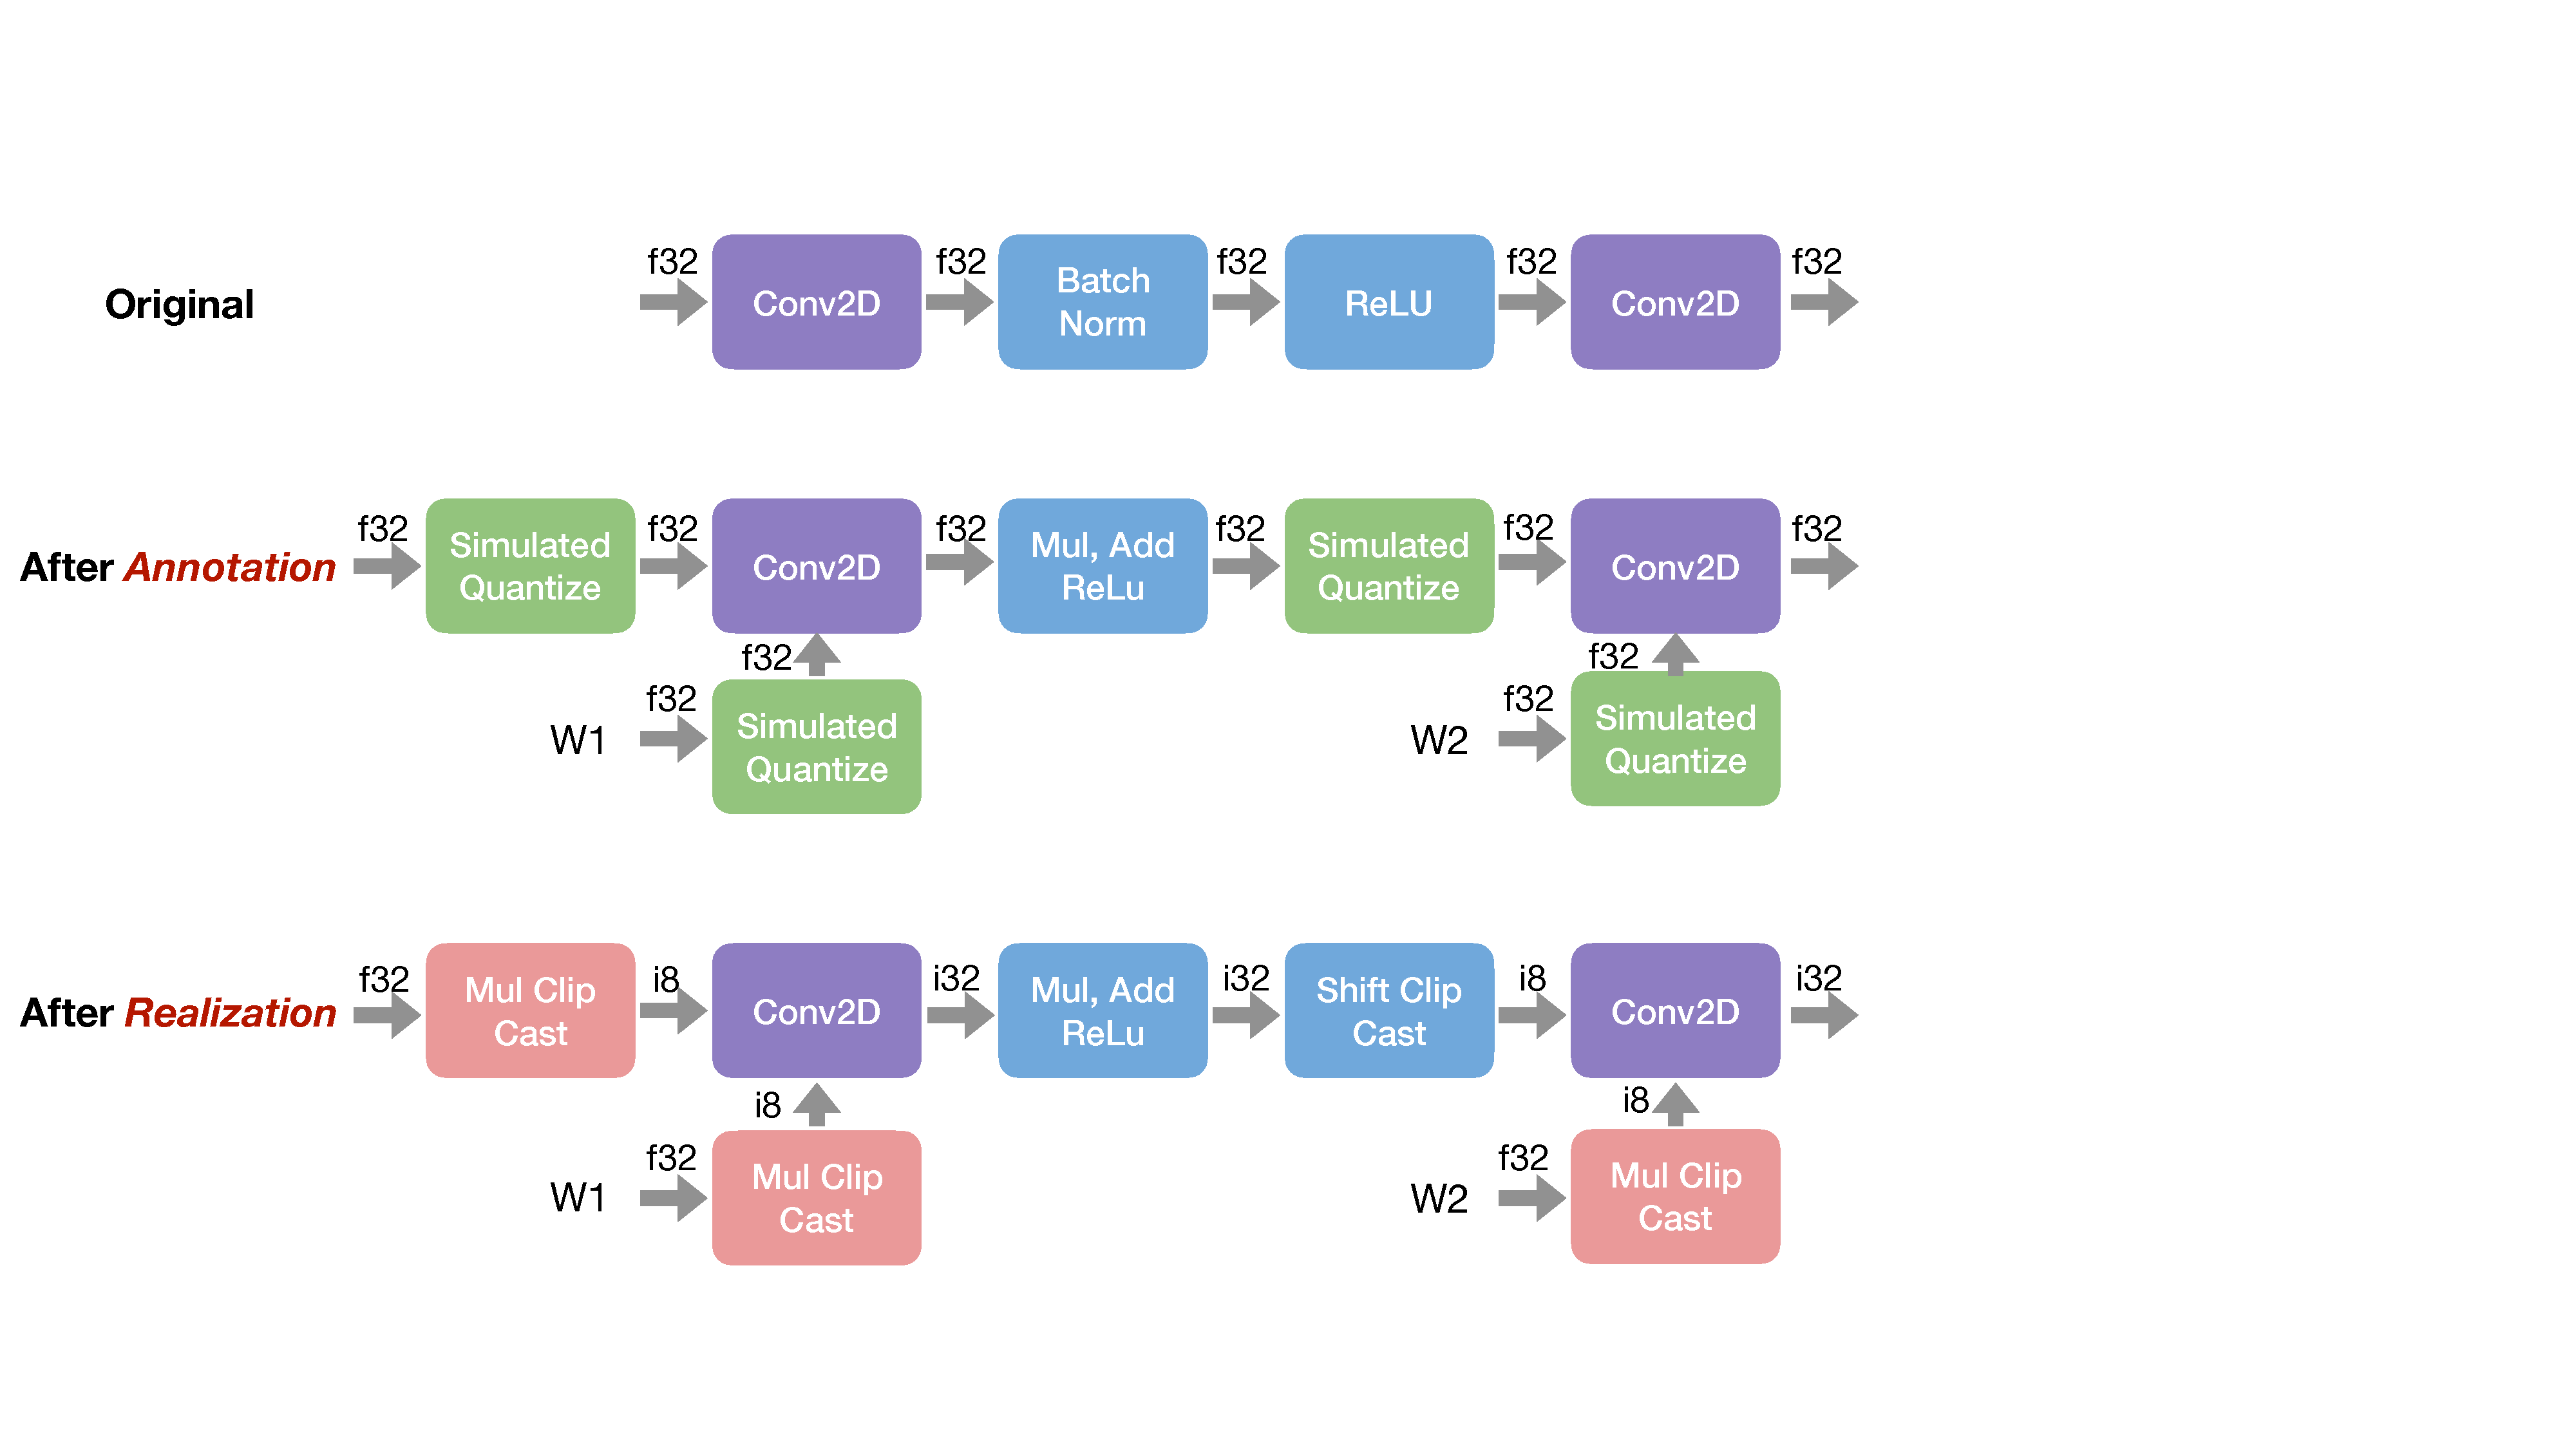
\includegraphics[height=5cm]{fig_splash19/quantization/quant_pdf.pdf}
  \caption{The top graph represents the dataflow graph of operators after annotation,
  and the bottom graph represents the transformed graph.
  SimQ simulates the rounding error and saturating error of quantizing.
  Its argument will get tuned during calibration.}
  \label{fig:quant_flow}
\end{figure}

\begin{figure}[h]
    \begin{equation}
      \begin{aligned}[b]
        \scriptscriptstyle
        & Q(x, r, bit, sign) =\\ & cast(clip(round(x/r*2^{bit-sign}), int8)) \\
      \end{aligned}
    \end{equation}
    \caption{The quantization operation.}
    \label{fig:quant_op}
    \begin{equation}
      \begin{aligned}[b]
        \scriptscriptstyle
        & sim\mathcal{Q}(bits, sign, range) =\\ & \dfrac{clip(round(\dfrac{x}{r} * 2^{bit - sign})) * r}{2^{bit - sign}}
      \end{aligned}
    \end{equation}
    \caption{The simulated quantization operation.}
    \label{fig:sim_quant_op}
\end{figure}

The generic quantization flow proceeds in three steps: annotation, calibration, and realization. We
can apply this pass to convolution-like operators which have a quantized schedule
available. Figure \ref{fig:quant_flow} shows a graphical visualization for this.

\paragraph{Annotate}

Annotation rewrites the program by inserting simulated quantization operations a
  according to an annotation rule of each operator.
The annotation rule describes how to transform an unquantified operation
  into a quantized one.
Each input or output to be quantized is passed to \texttt{sim$Q$},
  an operator that simulates the effect of quantization (for example, from a 32-bit
  floating point value to an 8-bit integer value).

See the definition of simulated quantize, as in Figure \ref{fig:quant_flow}.
We annotate the inputs to this operation with an operator $sim\mathcal{Q}$,
  which simulates the effect of quantization (for example, from a 32-bit
  floating point value to an 8-bit integer value).
However, it is computed with a 32-bit float data type, which is convenient for the
  calibration pass and debugging.
$sim\mathcal{Q}$ has a set of parameters that must then be calibrated in order to
correctly quantize the graph, namely the bits, the scale, and the range.
Finally, after the algorithm has selected
  appropriate setting for these parameters, it applies realization,
  which transforms the simulated quantization operator into the numerator.

% By computing on the unquantized type, Relay can later calibrate the parameters to
%   \texttt{sim$Q$} a necessary step to preserve accuracy of the model.
% \[
%   \texttt{sim$Q$}\left(x, \beta, \sigma, \rho\right) = \dfrac{\texttt{clip}\left(\texttt{round}\left(x / \rho \cdot 2^{\beta - \sigma}\right)\right) \cdot \rho}{2^{\beta - \sigma}}
% \]

\subsection{Calibrate}
The simulated quantized operations have a set of parameters which must
  be calibrated in order to correctly quantize the graph to achieve the
  minimal decrease in accuracy.
As seen above \texttt{sim$Q$} has an input $x$, as well as a number of parameters
  $\beta$, $\sigma$, and $\rho$.
\texttt{sim$Q$}'s parameters control the mapping between the quantized and unquantized type
  and must be calibrated, without calibration the model can be wildly inaccurate.
We must perform an auxiliary optimization task to find the appropriate
  setting for these parameters.
The Relay compiler supports a variety of strategies for setting these
  parameters.
The first strategy implemented is a hyper parameter sweep of a
  single global scale until such a scale is found that does not result
  in overflow.
Another approach is a vision specific scheme which uses
  a per-channel scale, and optimizes the scales using a
  simple mean-squared error loss.
Finally an approach adopted from MxNet uses a
  KL-divergence based loss to optimize the
  quantization scales.

\subsection{Realize}

\begin{table*}[t]
  \begin{tabular}{|c|c||c|c||c|c|}
    \hline
    \multicolumn{2}{|c}{\textbf{ResNet-18}} & \multicolumn{2}{c}{\textbf{MobileNet V2}} & \multicolumn{2}{c|}{\textbf{Inception V3}} \\
    \multicolumn{1}{|c}{Quant.}    & \multicolumn{1}{c}{Accuracy}   &  \multicolumn{1}{c}{Quant.}  & \multicolumn{1}{c}{Accuracy}  & \multicolumn{1}{c}{Quant.}  & \multicolumn{1}{c|}{Accuracy} \\
    \hline
    \texttt{float32} & 70.7 \%    & \texttt{float32} & 70.9 \%       & \texttt{float32} & 76.6 \% \\
    8/16         & 69.4 \%    & 8/32         & 66.9 \%       & 16/32        & 76.6 \% \\
    8/32         & 69.4 \%    & 8/16         & 66.9 \%       & 8/32         & 75.2 \% \\
    \hline
  \end{tabular}
  \caption{This table shows the accuracy of various quantized models.
    \texttt{float32} refers to the non-quantized model.
    Notation as in ``8/16`` refers to 8-bit quantization,
    16-bit accumulation}
  \label{fig:quant_results}
\end{table*}

The realization pass transforms the simulated quantized graph
  (which uses 32-bit floats)
  into a real low-precision computation graph.
The simulated quantized operator is transformed
  into several fine-grained operations like multiplication and addition.
This transforms the \texttt{sim$Q$} operator into the below quantization operator.
\[
  Q\left(x, \rho, \beta, \sigma\right) = \texttt{cast}\left(\texttt{clip}\left(\texttt{round}\left(x / \rho \cdot 2^{\beta-\sigma}\right), \texttt{qtype}\right)\right)
\]
Due to Relay's handling of fusion
  we are able fuse these scaling operations directly into
  to the original operator, transforming a convolution
  from \verb|fp32| to a type such as \verb|int4|.

To avoid the overflow, it also would be better to use larger global scale.
 With flexible configure, our workflow can be customized as best strategy for
 different networks and hardwares.
Quantized models require low-precision operators for efficiency. Due to our operator representation,
and the ability to leverage AutoTVM, TVM's auto tuner, we can automatic generate kernels for arbitrary
types without effort.

\begin{figure}[t]
  \begin{minted}[fontsize=\footnotesize]{python}
  @register_annotate_function("nn.conv2d", override=True)
  def annotate_conv2d(ref_call, new_args, ctx):
      lhs, rhs = new_args
      lhs = attach_simulated_quantize(lhs, sign=False, rounding='round')
      rhs = attach_simulated_quantize(lhs, sign=False, rounding='stochastic_round')
      return expr.Call(ref_call.op, [lhs, rhs], ref_call.attrs)
  \end{minted}
  \caption{
    An example of overloading the annotation function for 2-d convolution.
    In this example we treat both input, and the weights as unsigned integers,
    applying rounding to the input, and stochastic rounding to the weights.}
  \label{fig:annotate_conv}
\end{figure}

Developers can customize quantization with very little code.
For example, the quantization annotation function may be overloaded for any operation,
  making use of signed or unsigned integers, or different rounding strategies, such as
  floor, ceiling, or even stochastic rounding (Figure~\ref{fig:annotate_conv}).

To demonstrate the effectiveness of our generic quantization,
  we use Relay to explore
  different choices of input and accumulation bits.
The results are shown in Table~\ref{fig:quant_results}.
We find that no single strategy fits all use cases.
For certain network architectures such as MobileNet and ResNet, 16-bit to 32-bit
  quantization provides good accuracy,
   but 8-bit to 16-bit provides the best speedup,
  assuming the input does not overflow.
The current framework demonstrates the importance of applying
  various quantization schemes based on networks and hardware platforms.

  \subsection{Quantized Inference on ARM Platforms}
  To demonstrate the effectiveness of our generic quantization (see Section~\ref{sec:quant}),
    we use Relay to evaluate both \textit{accuracy} and \textit{performance} of different
    quantization schemes on vision workloads.
  To evaluate \textit{accuracy},
    we tested various quantization schemes
    (denoted $m/n$ for $m$-bit quantization and $n$-bit accumulation)
    against a \texttt{float32} baseline on three vision models,
    as shown in the table below:
  \begin{center}
    \begin{tabular}{|c|c||c|c||c|c|}
      \hline
      \multicolumn{2}{|c}{\textbf{ResNet-18}} & \multicolumn{2}{c}{\textbf{MobileNet V2}} & \multicolumn{2}{c|}{\textbf{Inception V3}} \\
      \multicolumn{1}{|c}{QS}    & \multicolumn{1}{c}{Acc.}   &  \multicolumn{1}{c}{QS}  & \multicolumn{1}{c}{Acc.}  & \multicolumn{1}{c}{QS}  & \multicolumn{1}{c|}{Acc.} \\
      \hline
      \texttt{fp32} & 70.7 \%    & \texttt{fp32} & 70.9 \%       & \texttt{fp32} & 76.6 \% \\
      8/32         & 69.4 \%    & 8/32         & 66.9 \%       & 16/32        & 76.6 \% \\
      8/32         & 69.4 \%    & 8/16         & 66.9 \%       & 8/32         & 75.2 \% \\
      \hline
    \end{tabular}
  \end{center}
  Figure~\ref{fig:portability-eval} shows the results of different
    levels of quantization on \textit{performance} when applied to the Raspberry Pi 3
    and Firefly RK3399 ARM-based platforms.
  The numbers show that as we opt for a more aggressive quantization scheme
    (e.g., 8/16),
    we achieve much improved performance with hardly a drop in accuracy.
  Interestingly,
    on some model/platform pairs,
    the \texttt{int8/int32} scheme performs slightly worse than \texttt{float32} on both platforms,
    which likely stems from the existence of faster hardware intrinsics for 16-bit operations on these systems.

% \begin{figure*}[htbp!]
%   \centering
%   % TODO: These graphs seem a little small.  Is there any more space hacking we can do?
%   \includegraphics[scale=0.53]{fig_splash19/eval/graph/quant_comp/raspberry_pi_quantization.png}
%   \hspace{-0.075in}
%   \includegraphics[scale=0.53]{fig_splash19/eval/graph/quant_comp/rk3399_quantization.png}
%   % TODO: Use real numbers for this.
%   \includegraphics[scale=0.53]{fig_splash19/eval/graph/fpga_comp/fpga_eval.png}
%   \caption{\textmd{
%     \textit{(left)} Inference time of vision DNNs on low-power platforms using
%       different data types.
%     Relay allows us to reduce inference time on power-constrained devices by
%       easily substituting \texttt{float32} multiplications with \texttt{int8}
%       multiplications and \texttt{int16} or \texttt{int32} accumulations (denoted
%       as \texttt{int8}/\texttt{int16} and \texttt{int8}/\texttt{int32}, respectively).
%     We used 1000 trials for each model.
%     \textit{(right)}
%     Batch-size-normalized inference time of vision DNNs and a TreeLSTM running on two DNN accelerator variants implemented on an edge FPGA.
%     One accelerator performs single-batch inference, while the other implements multi-batch inference.
%     % Multi-batch inference provides tangible throughput improvements on TreeLSTM due to the memory bandwidth constrained nature of the workload.
%     The two hardware designs have the same number of compute units that are arranged differently to take advantage of different types of tensor computation.
%     Relay applies a multitude of graph-level transformations required to run different workloads onto these DNN hardware designs.
%     We used 12 trials for each model.
%   }}
%   \label{fig:portability-eval}
% \end{figure*}

\section{Partial Evaluator}
\label{sec:partial_eval}
Existing deep learning IRs have relied on
  a mixture of staging and constant evaluation
  in order to optimize user programs.
Partial evaluation is a generalized form of constant
  evaluation that can reduce partially constant
  programs.
A partial evaluator (PE) allows the use of high-level abstractions
  without limiting code that \textit{could} in practice be
  compiled to a particular target.
Relay is the first compiler to apply partial evaluation
  techniques to deep learning, the
  core approach of which is based on \citep{pe_ref}.
Partial evaluation, when composed with other
  optimizations like fusion, yields a variety
  of useful optimizations without requiring
  a separate implementation of each.
For example, the partial evaluator can be used to perform
  loop unrolling, which then enables further fusion,
  without any additional compiler passes.
We describe the implementation and some
  concrete applications of partial evaluation
  in Chapter~\ref{ch:ad}.

\section{Dynamic Memory Allocation, Device Placement, and Code Generation}

A key challenge preventing existing deep learning compilers from handling dynamism
  is the lack of a uniform and dynamic representation.
For example, optimizations and runtime of existing IRs,
  e.g., TVM's NNVM~\citep{tvm_osdi18}, always assume the presence of static shape information.
These assumptions introduce quite a few challenges for optimizing dynamic behaviors.
This section describes how we transform standard TVM programs into our dynamic dialect
  which enables us to easily apply static optimizations to dynamic programs, much as we
  do in traditional compiler optimization.
Particularly, we detail three key components required to compile dynamic models.

\begin{itemize}
    \item An extended type system which enables static tracking of dynamic shapes.
    \item A series of optimization passes that make dynamic output shapes, allocation, and device placement explicit.
    \item A set of code generation techniques for producing code of kernels with dynamic input and output shapes.
\end{itemize}

\subsection{Dynamic Memory Planning}
\label{subsec:optimizations:memory}

Deep learning workloads are dominated by two key aspects,
  compute-intensive kernels and memory allocation.
Many deep learning compilers use a form of static memory planning which tries to
  coalesce memory and minimize allocations.
For devices such as GPUs these optimizations are essential for reducing memory fragmentation and ensuring allocation
  does not hamper kernel performance. E
Existing deep learning compiler IRs hide memory allocation behind a functional interface,
  where each operator implicitly allocates their output storage.
Then before execution, the system performs static-memory planning on the data-flow graph enabling efficient pre-allocation of the required memory. Due to this ``out-of-band'' nature of memory allocation, it is challenging to customize, modify or compose memory optimizations with other passes. For example, if one needs to adjust memory allocation for heterogeneous execution, modifications to the runtime are required.

Deep learning workloads are dominated by two key components,
    compute-intensive kernels and memory allocation.
Many deep learning compilers use a form of static memory planning
    coalesces memory into contiguous chunks and minimize allocations.
For devices such as GPUs these optimizations are essential for
    reducing memory fragmentation and ensuring allocation does not hamper kernel performance.
Existing deep learning compiler IRs hide memory allocation behind a
    functional interface, where each operator implicitly allocates their output storage.
Then before execution, the system performs static-memory planning on the data
    flow graph enabling efficient pre-allocation of the required output buffers.
Due to this ``out-of-band'' nature of memory allocation,
    it is challenging to customize, modify, or compose memory optimizations with other passes.
For example, if one needs to adjust memory allocation for heterogeneous execution,
    modifications to the runtime system are required.
TVM's graph runtime is one such example of static memory planning.
Due to the coarse-grained memory semantics of deep learning models,
    it is essential that memory optimizations occur at a suitably high-level of abstraction,
    unlike traditional compilers.
Existing work provides no clear path to performing static optimization on dynamic memory
    allocation.

Alternatively, some systems lower the entire program to low-level IRs such as
  LLVM~\citep{llvm} in order to perform optimizations.
Due to the coarse-grained memory semantics of deep learning models,
  it is essential that memory optimizations occur at a suitably high-level of abstraction before essential program facts are lost.
Moreover, as discussed in~\autoref{sec:compilation:shape-func}, we have introduced new ways to account for the handling of dynamic allocations,
  which further complicate memory analysis.
In order to perform dynamic memory planning we have extended TVM's Relay IR,
  using these extensions we translate a IR dialect where all memory allocations are
  implicit to one where buffers are allocated and passed around explicitly.
  The key to this transformation is an inter-procedural change of calling convention,
  with each operator now taking its outputs explicitly it is possible to track and transform allocations.
In particular, we have introduced four new IR constructs,
  (a) \verb|invoke_mut(op, inputs, outputs)| which takes outputs as mutable in-out arguments,
  (b) \texttt{alloc\_storage(size, alignment, device)} which allocates a region of memory of a particular size,
  (c) \texttt{alloc\_tensor(storage, offset, shape, dtype, attrs)} which allocates a tensor at a particular storage offset
    with a shape and data type, and
  (d) \verb|kill(tensor)| which frees a tensor before its reference count becomes zero due to exiting the frame.
Note that in the below code examples \texttt{Tensor<d1, ..., dn>}
is shorthand for a tensor of shape \texttt{(d1, ..., dn)} containing floating point values.

We can demonstrate how to transform a single statically shaped operation such as broadcasting addition.

\begin{minted}{rust}
fn main() -> Tensor<10> {
  let t1, t2 : Tensor<10> = ...;
  add(t1, t2)
}
\end{minted}

Here we only must allocate a single buffer, the return buffer for the addition operation.

\begin{minted}{rust}
fn main() -> Tensor<10> {
  let t1 = ...; let t2 = ...;
  let storage = alloc_storage(40, 64, cpu(0));
  let out1= alloc_tensor(storage, 0, (10), f32);
  invoke_mut(add, (t1, t2), (out1));
  out1
}
\end{minted}

The above transformation replaces all operator invocations with a call to \verb|invoke_mut| allocating storage
for backing a single tensor from allocated at offset zero.
The key insight is to internalize a notion of memory allocation into the IR, enabling static optimization of
both static and dynamic allocations presence of control and dynamic shapes. We realize our shape functions as fragments of TVM's tensor expression language which computes the output shape for a particular operator. As detailed in~\autoref{sec:compilation:shape-func} our shape functions may require the input, the input \textit{shape}, or both.
Our uniform treatment of shape functions as standard tensor expressions enables them to be fused and optimized like normal, but one challenge is that we must now manifest allocations in a fixed point until we allocate for both the compute and necessary shape functions. We illustrate this below with a single dynamic concatenation.

\begin{minted}{rust}
fn (x: Tensor<?,2>, y: Tensor<1,2>)->Tensor<?,2> {
  concat((%x, %y))
}
\end{minted}

This is the same transformation as the previous example with the addition of carefully inserting
invocations to the shape function to compute output buffers sizes for the dynamically sized kernel.

\begin{minted}{rust}
fn (x: Tensor<?,2>, y: Tensor<1,2>)->Tensor<?,2> {
  let in_sh0 = shape_of(x);
  let in_sh1 = shape_of(y);
  let storage_0 = alloc_storage(16, 64, ...);
  let out_sh0 = alloc_tensor(storage_0, ...);
  invoke_shape_func(concat,
      (in_sh0, in_sh1), (out_sh0,), ...);
  let storage_01 = alloc_storage(...);
  let out_0 = alloc_tensor(
      storage_01, shape_func_out_0, ...);
  invoke_mut(concat, (x, y), (out_0));
  out_0
}
\end{minted}

After the transformation you may notice we have introduced calls to \verb|shape_func| which
  invokes a shape function for a kernel.
The shape function requires input shapes as arguments which further require us to invoke \verb|shape_of|
  for both \verb|%x| and \verb|%y|.
\verb|shape_of| will be directly mapped to a VM instruction to retrieve the shape of a tensor at runtime.
More description of it will be provided in \autoref{sec:compliation:hetero}.

Now that the all allocations are explicit in the IR we can provide analogous optimizations in the static
case on dynamic programs, for example we have implemented a storage coalescing pass which groups storage
into a larger region which we can then multiplex tensor allocations on to.

For the sake of space, we present a more complex example in the \autoref{appx:mem-plan-example},
  which illustrates how to handle memory allocation when operators have dynamic shaped inputs.
The key insight is to internalize a notion of memory allocation into the IR,
  enabling static optimization of both static and dynamic allocations in the presence of control and dynamic shapes.
Now that all allocations are explicit in the IR, we can provide analogous optimizations in the static case on dynamic programs,
  for example we have implemented a storage coalescing pass to group storage
  into a larger region which allows the multiplexing of multiple tensor allocations to a single piece of storage.
Further optimization like liveness analysis and graph coloring algorithm can be applied to the program to reuse the storages.

\subsection{Heterogeneous Device Placement}
\label{sec:optimizations:hetero}

As discussed in Section \autoref{sec:compilation:shape-func}, shape functions are executed at runtime to
  calculate the output shape of an operator.
These functions must execute on the CPU due to the host-interaction model of GPU like devices.
In the case of heterogeneous execution (i.e., CPU and GPU) it is essential to carefully schedule
  the execution of shape functions and kernels as improper scheduling can be disastrous for performance.
For instance, considerable overhead will occur if inputs to shape functions must be copied from
  GPU due to the cost of data transfers and synchronization.
To minimize the performance penalty, we analyze the program allocations to place sub-expressions on the most suitable devices.

We introduce a unification based analysis for computing the correct device placement and
  allocation based on the previous scheduling of the compute kernels.
The goal of our device analysis is assigning each IR node in a way that minimizes
  the number of cross-device copies. We introduce a concept of \texttt{DeviceDomain}
  to represent the domain of a device, including source and destination.
Each expression in the IR defaults to the empty domain, meaning there
  are no constraints on its device placement.
In addition, two new IR constructs are introduced to facilitate the heterogeneous execution of VM,
  namely \verb|device_copy| and \verb|shape_of|.
The former performs a data transfer between different devices and is
  inserted when a cross-device data copy is mandatory.
The latter is used to retrieve the shape of a tensor at runtime and is
  used to efficiently compute the input shapes for shape functions.
Our analysis is formulated as a set of device placement rules which describe how device constraints
  flow, and then we use unification, a technique common in type inference and compilers
  in order to compute precise device placement.

As discussed in \autoref{sec:compilation:shape-func},
  shape functions are executed at runtime to calculate the output shape of an operator.
These functions should execute on the CPU as their outputs are used to compute the size of allocated memory.
In the case of heterogeneous execution (i.e., CPU and GPU),
  it is essential to carefully place the execution of IR nodes to proper devices.
Otherwise, considerable overhead from data transfers and device synchronization will
  occur if the inputs to shape functions and kernels need to be copied from or to GPU.
To minimize the performance penalty, we analyze the program to place sub-expressions on the most suitable devices.

We introduce a unification based analysis for computing the correct device placement
  and allocation based on the previous scheduling of the compute kernels.
The goal of our device analysis is to assign each IR node properly to minimize
  the number of cross-device copies.
We introduce a concept of \texttt{DeviceDomain} to represent the domain of a device,
  including source and destination.
Each expression in the IR defaults to the empty domain, meaning no constraint on its device placement.
In addition, a new IR construct, \verb|device_copy|, is introduced to facilitate the heterogeneous execution
  of the Relay VM runtime.
It represents a data transfer between different devices and is inserted when a cross-device data copy is mandatory.
%The latter\yida{what does this refer to?} is used to retrieve the shape of a tensor at runtime and is used to efficiently compute the input shapes for shape functions.
Our analysis is formulated as a set of device placement rules which describes how device constraints flow, and then we use unification, a technique common in type inference and compilers, to compute the precise device placement.
\autoref{fig:hetero} depicts some highlights of the rules to assign and propagate the device types: (a) both inputs and outputs of shape function are assigned to CPU, (b) the output of \verb|device_copy| is assigned to the device that is copied to, (c) all arguments to \verb|invoke_mut| should have the same device domain. The full set of rules can be found in the \autoref{appx:hetero-rules}.

\begin{itemize}
    \item \verb|shape_of|. Defaults to the CPU domain because we can access a Tensor's shape regardless of which device it is placed on.
    \item Shape functions. These IRs take the output of one or multiple \verb|shape_of| and then derive the shape of an operation according to predefined type inference rules. The output of a shape function is used to compute the amount of memory that this operator requires at runtime, which only needs a few cheap scalar arithmetic computation. Therefore, the inputs and outputs would be better on a CPU domain as well.
    \item \verb|device_copy|. The input and output of this IR are on different domains as it copies data from one domain to another. The device domains of the input and output are propagated in the opposite directions to other IR nodes that are reachable to/from the device copy node.
    \item Memory operations. The device domain of storage from \verb|alloc_storage| is designated in the expression, and later is propagated to the device domain of the tensors allocated from this storage via \verb|alloc_tensor|.
    %in the instruction computation of the allocation size and the shape for memory operations, such as \verb|alloc_storage| and \verb|alloc_tensor|, should be on CPU due to low computation intensity.
    \item \verb|invoke_mut|. All arguments used in the \verb|invoke_mut| must have the same device domain.
    \item Other common IR nodes. The device domain of other common IR nodes, e.g. variables, constants, operators, etc., can be directly propagated from the above nodes.
\end{itemize}


% \begin{figure}
%     \centering
%     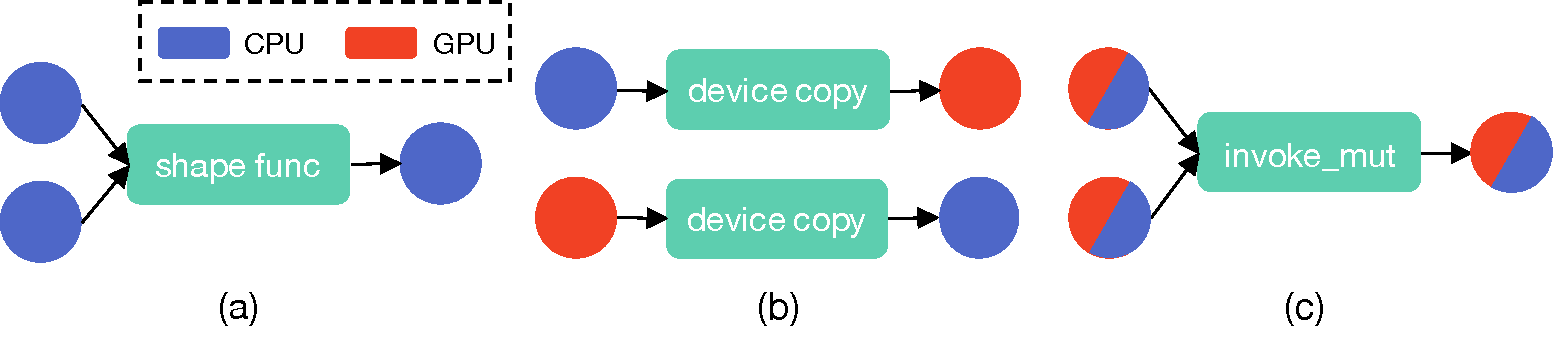
\includegraphics[width=\linewidth]{figs/hetero.pdf}
%     \caption{Some heterogeneous device placement rules. (a) The inputs and outputs of shape functions are placed on CPU.
%     (b) \texttt{device\_copy} changes the device of output accordingly.
%     (c) The device of all arguments to \texttt{invoke\_mut} must be the same.
%     }
%     \label{fig:hetero}
%
% \end{figure}

Based on the rules defined above, we use a union-find data structure to bidirectionally
  propagate and unify the device placement of each IR node.
We introduce two operations, \texttt{union(s, t)} and \texttt{find(s)},
  to achieve \texttt{DeviceDomain} unification throughout the entire program.
\texttt{union(s,t)} unions the equivalence device domains of \texttt{s} and \texttt{t}
  into one equivalence domain when the device types match.
\texttt{find(s)} returns the representative of the device domain
  that \texttt{s} belongs to.
These two operations are applied until all IR nodes are annotated.
The result of the heterogeneous device placement composes with memory planning
  and shape function insertion resulting in correctly placed allocations.
Based on these rules, we use a union-find data structure to
  bidirectionally propagate and unify the device placement of each IR node.
We introduce two operations, \texttt{union(s, t)} and \texttt{find(s)},
  to achieve \texttt{DeviceDomain} unification throughout the entire program.
\texttt{union(s,t)} unions the equivalence device domains of \texttt{s}
  and \texttt{t} into one equivalence domain when the device types match.
\texttt{find(s)} returns the representative of the device domain that \texttt{s} belongs to.
These two operations are applied until all IR nodes are annotated.
The result of the heterogeneous device placement composes with memory planning and shape function insertion resulting in
correctly placed allocations.

\subsection{Dynamic Kernel Code Generation}
\label{sec:compliation:codegen}
Deep learning compilers~\citep{tvm_osdi18, halide} have demonstrated competitive performance compared to manually
  tuned kernels on multiple platforms.
Recent trends apply machine learning based search to further reduce or eliminate complex manual performance tuning,
  existing work applies both template based~\citep{chen2018learning, zheng2020flextensor} and beam search based~\citep{adams2019learning} ones.

However existing work which focuses on tuning in the presence of static shapes falls short with symbolic or dynamic shapes.
There are two inherent challenges with regard to performing code generation for symbolic shapes.
\begin{itemize}
    \item How to achieve the same performance of kernels generated with symbolic shapes as that with static shapes when applying the same schedule?
    \item How to extend the machine learning based approach to tune kernels with symbolic shapes?
\end{itemize}

% %\yida{Should we mention the mechanism of invoking third-party libraries in this subsection?}
% Deep learning compilers~\citep{tvm_osdi18, halide} have demonstrated competitive performance compared to manually tuned kernels on multiple platforms. Recent trends apply machine learning based search to further reduce or eliminate complex manual performance tuning using either template based~\citep{chen2018learning, zheng2020flextensor} or search based~\citep{adams2019learning, zheng2020ansor} approaches.
% However, existing work which focuses on tuning in the presence of static shapes falls short with symbolic or dynamic shapes. There are two inherent challenges with regard to codegen of symbolic shapes.
% %\begin{itemize}
% %    \itemsep 0em
% \squishlist
%     \item How to achieve the same performance of kernels generated with symbolic shapes as that with static shapes when applying the same schedule?
%     \item How to extend the machine learning based approach to tune kernels with symbolic shapes?
% \squishend
%
% %\end{itemize}

% Our codegen approach for dynamic shapes is designed to integrate well with TVM's codegen. We implement a bucketing
% based codegen strategy, which generates a set of shape-specialized variants and code which selects between them. One
% attractive consequence of this design is that it allows us to integrates with the current version of AutoTVM~\citep{chen2018learning}, TVM's auto-tuning framework
% to further optimize kernels.


Loop parallelism and loop tiling are common optimization techniques that exploit multi-core capabilities by achieving data access patterns which
  are memory hierarchy aware for both CPUs and GPUs. However, the combination of these techniques lead to complex loop boundary conditions.
In many static cases, it is possible to prove these conditions always hold, and thus eliminate checks which hamper further optimizations such as unrolling.
While straightforward to handle with static shapes, it becomes a non-trivial challenge when performing symbolic codegen.
If not carefully handled, the boundary condition checks will stay, leading to poor performance.

To address this issue, we generate multiple kernels according to the residues modulo of the tiling
  factor and then dispatch based on the actual shape at runtime.
For example, suppose a symbolic dimension $x$ is divided by a factor of 8, we then duplicate the generated kernel
  for 8 times, and replace the symbolic var $x$ by $8k+r$ in each copy, where $k = \lfloor x / 8 \rfloor$ and $r \in [0..7]$.
By applying this technique in conjunction with an enhanced symbolic expression simplification pass,
  we can eliminate most boundary checks to achieve performance that is nearly identical
  to kernels compiled with a single static shape.
Lastly, we automatically generate a dispatch function that invokes the corresponding kernel based on the residue.

% Loop parallelism and loop tiling are common optimization techniques that exploit multi-core capabilities by achieving data access patterns which are memory hierarchy aware for both CPUs and GPUs. However, the combination of these techniques lead to complex loop boundary conditions. In many static cases, it is possible to prove these conditions always hold, and thus eliminate checks which hamper further optimizations such as unrolling.
% While straightforward to handle with static shapes, it becomes a non-trivial challenge when performing symbolic codegen. If not carefully handled, the boundary condition checks will stay, leading to poor performance.

% To address this issue, we generate multiple kernels according to the residues modulo of the tiling factor and then dispatch based on the actual shape at runtime.
% For example, suppose a symbolic dimension $x$ is tiled by a factor of 8, we then duplicate the generated kernel for 8 times, and replace the symbolic var $x$ by $8k+r$ in each copy, where $k = \lfloor x / 8 \rfloor$ and $r \in [0..7]$. By applying this technique in conjunction with an enhanced symbolic expression simplification pass, we can eliminate most boundary checks to achieve performance that is nearly identical to kernels compiled with a single static shape. Lastly, we automatically generate a dispatch function that invokes the corresponding kernel based on the residue.
% %because this function is also generated in the IR we can compile and optimize it like other code ahead of time.
% In addition, the dispatch function can be extended to invoke either compiler generated kernels or {\em third party library} whichever is faster from the profiling results.
% The increased kernel size is relatively small compared to the overall deep learning models.
% In case where resources are extremely limited, we can either generate fewer number of kernels than the tiling factor or reduce the tiling factor to find an acceptable trade-off between code size and performance.

% A known issue to machine learning based tuning is that it may take a long time (usually hours) to find the best schedule for a single kernel. When it comes to symbolic shapes, the tuning time may be exponentially longer if we naively tune for every possible shape. In this paper, we extend the template based tuning approach for symbolic shapes to make tuning time tractable. The template based tuning approach takes a human-defined code template and a search space, and searches the best configuration within the search space by using machine learning algorithms.
% %by building on the techniques explored in based~\citep{chen2018learning}.
% We observe that a good configuration for one shape usually performs well on other shapes. Based on this observation, we devise the following mechanism to tune the kernel for symbolic shapes.


% \begin{enumerate}
%     \itemsep 0em
%     \item First replace the symbolic dimensions by a large enough value (e.g., 64) so that the search space can cover most possibilities, and run the tuning algorithm on the static shape for a sufficient number of iterations.
%     %
%     \item Pick top $k$ configurations, apply them to a selection of other shapes, and evaluate their performance.
%     %
%     \item Pick the configuration that performs best on average among shapes previously evaluated.
% \end{enumerate}

% Empirically, we found that $k=100$ covers most of the best configurations for other shapes. Current popular dynamic models usually only require kernels with one symbolic variable. As a result, we choose the values of power of two up to 256 in the cross evaluation of other shapes. If there is more than one symbolic variable, a more sophisticated selection approach might be required to limit the evaluation time of step 2. We leave this to the future work. Further, if the workload distribution is known, we can adjust the weighting of known shapes in step 3.

% %Though we address both challenges, we admit that our approach has limitations when all dimensions are unknown. In these cases symbolic codegen cannot completely replace manually tuned 3rd party libraries yet, but is complimentary when partial shapes are known.\yida{Can we remove this paragraph?}


In addition, the dispatch function can be extended to invoke either compiler generated kernels
  or third party library whichever is faster from the profiling results.
The increased kernel size is relatively small compared to the overall deep learning models.
In extreme cases where resources are extremely limited,
  we can either generate fewer number of kernels than the tiling factor
  or reduce the tiling factor to find an acceptable trade-off
  between code size and performance.

A known issue to machine learning based tuning is that it may take a long time (usually hours) to find
  the best schedule for a single kernel.
When it comes to symbolic shapes, the tuning time may be exponentially longer if we
  naively tune for every possible shape.
In this paper, we extend the template based tuning approach for
  symbolic shapes in order to make tuning time tractable.
The template based tuning approach takes a human-defined
  code template and a search space, and searches the best configure
  within the search space by using machine learning algorithms.
We observe that a good configuration for one shape usually performs
  well on other shapes.
Based on this observation, we devise the following mechanism
  to tune the kernel for symbolic shapes.

\begin{enumerate}
    \item First replace the symbolic dimensions by a large enough value (e.g., 64) such that the search space can cover most possibilities, and run the tuning algorithm on the static shape for a sufficient number of iterations.
    \item Pick top $k$ configurations, apply them to a selection of other shapes, and evaluate their performance.
    \item Pick the configuration that performs best on average among shapes previously evaluated.
\end{enumerate}

We found that $k=100$ covers most of the best configurations for other shapes.
Current popular dynamic models usually only require kernels with one symbolic variable.
As a result, we choose the values of power of two up to 256 in the cross evaluation of other shapes.
If there is more than one symbolic variable, a more sophisticated selection approach might be
  required to limit the evaluation time of step 2.
We leave this to the future work.
Further, if the workload distribution is known, we could adjust the weighting of known shapes when picking the best configuration for step 3.

% % Our codegen approach for dynamic shapes is designed to integrate well with TVM's codegen. We implement a bucketing
% % based codegen strategy, which generates a set of shape-specialized variants and code which selects between them. One
% % attractive consequence of this design is that it allows us to integrates with the current version of AutoTVM~\citep{chen2018learning}, TVM's auto-tuning framework
% % to further optimize kernels.

Though we address both challenges, we admit that our approach has limitations when all dimensions are unknown.
In these cases symbolic codegen cannot completely replace manually tuned 3rd party libraries yet,
  but is complimentary when partial shapes are known.

% When an operator appears with dynamic shape it often will only vary along a single dimension. We are able to handle cases that
% deal with imperfect tiling strategies but the critical performance piece is choosing a tuned operator with the appropriate tile size.
% We reuse the machinery of the VM to support invoking a bucketed operator. For each operator with a dynamic shape we will
% generate tile sizes for powers of two, and then for a given input size round to the nearest power of two tile size and select that operation.
% The code for selecting between buckets is also realized as TVM expression allowing further optimization of the combined kernel.
% This strategy can be viewed as a form of polymorphic inline caching~\citep{inline_caches}, where the cache is not keyed by type, but shape.

% % When an operator appears with dynamic shape it often will only vary along a single dimension. We are able to handle cases that
% % deal with imperfect tiling strategies but the critical performance piece is choosing a tuned operator with the appropriate tile size.
% % We reuse the machinery of the VM to support invoking a bucketed operator. For each operator with a dynamic shape we will
% % generate tile sizes for powers of two, and then for a given input size round to the nearest power of two tile size and select that operation.
% % The code for selecting between buckets is also realized as TVM expression allowing further optimization of the combined kernel.
% % This strategy can be viewed as a form of polymorphic inline caching~\citep{inline_caches}, where the cache is not keyed by type, but shape.

\section{Accelerator-Specific Optimizations}
\label{sec:accel-opts}

Many accelerates provide non-traditional programming
    abstractions to compilers and users.
For example many traditional platforms can have
    code generated via LLVM.
These simply expose an LLVM backend which generates
    a well known ISA.
Many accelerators are not programmable in this style
    and require a mixture of driver interactions
    and static and dynamic code generation to
    drive a program to compeletion.
Even on very popular accelerators such as GPU
    violate the typical CPU programming model.
In order to lower generic deep learning programs
    to these types of accelerators it is
    essential we are able to optimize programs.
For example some accelerators only support
    low-bit datatypes converting quantization
    from an optimization to a necessary program
    transformation.

Although DL accelerators form a diverse family of designs,
  one property they have in common is a restricted computing model.
The consequence of this is that individual accelerators
  can rarely execute entire Relay programs.
For example, some accelerators cannot execute unbounded loops,
  requiring individual computations to be scheduled via
  host device (often a CPU) which interacts with the device runtime
  as well as programming it.

Below we highlight a few of these optimizations that were used for
VTA discussed in section XXX, as well as accelerators supported by
TVM.

\textit{Axis scale folding} is an optimization that removes scaling
  operations that occur before or after convolution-like operators.
The multiplication by a scalar is moved through a convolution towards
  its constant inputs, such as parameters.
By moving the scaling operation to a constant weight, we are able
  to compute away the scale using the partial evaluator.
This optimization is required for certain accelerators that lack scalar multipliers~\citep{moreau2018vta}.
In order to target these accelerators,
  we must eliminate \textit{all} scalar operations.

\textit{Parallel convolution combination} is a specialized
  optimization that fuses multiple 2D convolutions that share the same input.
The goal of this pass is to produce a larger kernel for the GPU,
  as each kernel launch on the GPU has overhead.
It was designed with the Inception network \citep{inception} in mind, as it
  contains blocks of convolutions that share the same input.
The entire parallel convolution combination pass,
  including documentation and tests,
  required fewer than 350 lines of code and was contributed
  by a non-Relay affiliated undergraduate student
  in their first contribution to our codebase.

\section{Dataflow Rewriting}

A key portion of compiler optimization is
  the selection and application of rewrite rules for a variety
  of use cases.
Many of optimizations, especially those around program partitioning can
  be phrased a sequence of rewriting rules over a program or set of
  programs.
We have explored two very different rewriting approaches in TVM
  the first was specifying dataflow patterns for end users to
  match dataflow graph properties and select subgraphs.
The second was the use of Egg TODO a library
  for utilizing equivalence graphs to perform saturated rewriting.
We describe both approaches in the context of the TVM stack
  below.

\subsection{Dataflow Patterns}
TODO

\subsection{EggBeater: Egg + TVM}
TODO

% Should/Could merge into optimizations \chapter{Relay: virtual machine for executing tensor programs}
\label{ch:dynamic}

Relay's instruction set is designed as an abstract machine for executing tensor valued
computations. We can realize this abstract machine by either interpreting it or generating
machine code. This is a tried and true approach utilized by existing languages and languages
runtime such as Java, or C\#.

By lowering the full language to an abstract machine we can reduce it to its core operations,
resulting in a small set of operations we can implement. Our implementation uses a virtual
machine design over an ahead of time compiler. In traditional virtual machines the key
reason to perform ahead of time compilation is to reduce dispatch time, and specialize
away dynamic features such as virtual dispatch.

Due to the design of the Relay instruction set, instruction dispatch is a very minimal
part of the total runtime, the runtime is defined by kernel execution time.
A virtual machine allows easier experimentation and modification at the cost of dynamically
dispatching instructions, though nothing in our design prevents ahead of time compilation
of the instruction set, but it provides little value for this reason.

For example if we need to produce ahead of time
compiled code, we either must generate calls into a runtime system (which is dynamic),
only removing instruction dispatch, or statically schedule limiting flexibility and
extensibility.

Furthermore our use of TVM means all kernels are ahead of time compiled meaning the
code which dominates execution time, remember most kernels are quadratic or cubic in
complexity, have efficient implementations.

Our extensions for dynamically sized kernels also utilize TVM code generation, enabling
ahead compilation of kernels which perform a form of polymorphic inline caching for shapes,
playing a similar role to what an ahead of time compiler does in traditional JITs.



\subsection{Tensor Virtual Machine}

Although Relay defines an IR and formal semantics
  it does not provide an efficient execution mechanism for the full language.
In the tradition of definitional interpreters we introduced
  a simple interpreter for Relay which implements its formal semantics, which
  we have separately formalized.
Relay’s interpreter can execute the full language but has notable limitations
  that make it unsuited for production deployments.
It is structured as an inefficient interpreter that performs AST traversal to execute the program.
This approach is conceptually simple but inefficient, as the AST traversal heavily relies on indirection.
For example the initial Relay prototype reused the existing ``graph runtime'', to obtain
  acceptable performance for vision tasks.
The graph runtime can only execute simple control-free,
  DAGs of operations.
We can optimize Relay programs and map a subset of them
  to the graph runtime, but any use of new Relay features
  are unsupported.
By introducing models which make use of new features such
  as control flow, recursion, dynamic shapes, and dynamic allocation,
  we must change how execution works.
There are further challenges in compiling dynamic code, such as dynamic scheduling and allocation,
  fully dynamic tensor shapes, and control flow.
The interpreter offers simple solutions for these, but none is sufficiently compelling or optimized.
The simplicity of the graph runtime provides attractive
  properties such as simple serialization, straightforward
  optimal memory layout, and ease of deployment.

To address these challenges we designed a new Relay
  virtual machine.
The Relay virtual machine balances framework the competing approaches to execution,
  providing a dynamic execution environment which can be extended, instrumented, and integrated with other approaches
  like ahead-of-time compilation via a flexible extension mechanism.
The virtual machine is designed to strike a balance between performance and flexibility
  when deploying and executing Relay programs, without giving up the benefits of TVM.
Virtual machine (VM) design is a well-studied area in programming languages and systems,
  and there have been various virtual machine designs for both full-fledged and embedded programing languages.
Previous language VM designs have been heavily tailored to the execution profile of traditional programs.
Traditional programs manipulate small scalar values
  and consist of a large number of low-level instructions.
The sheer quantity of instructions requires instruction execution
  and dispatch to be extremely efficient.
In the context of machine learning we manipulate primarily tensor values,
  using a (relatively) low number of high level instructions.
ML programs’ cost centers are expensive operator invocations,
  such as GEMM or convolution, over a large input.
Due to the execution profile exhibited by ML programs,
  micro-optimizations present in scalar VMs are dramatically less important.

The Relay virtual machine implement a simple register based VM.

The VM consists of three pieces:
\begin{enumerate}
  \item A tensor instruction set for a tensor virtual machine.
  \item A compiler from Relay to the tensor VM.
  \item An implementation of the virtual machine.
\end{enumerate}

\subsection{ISA}
\begin{itemize}
    \item \verb|ret| Returns a value.
    \item \verb|invoke_packed| Invoke a packed function with the specified arguments.
    \item \verb|alloc_tensor| Allocate a tensor of the given size.
    \item \verb|alloc_datatype| Allocate a datatype with the fields.
    \item \verb|alloc_closure| Allocate a closure.
    \item \verb|get_field| Project a field.
    \item \verb|if| Conditional jump based on the condition register.
    \item \verb|get_tagi| Get the object's tag.
    \item \verb|fatal|
    \item \verb|invoke| Invoke a Relay function.
    \item \verb|invoke_closure| Invoke a Relay closure.
    \item \verb|load_const| Load a constant from the constant pool.
    \item \verb|int_const| Store a constant integer in destination.

\end{itemize}
\subsection{VM Compiler}

In order to execute on the VM we wrote a new compiler which
  can lower Relay directly on to the VM bytecode, and then
  executed.
The compiler performs a set of transformations on the high-level
  Relay program before generating code:
\begin{itemize}
  \item A-Normal Form, converts program in to a limited single-assignment form.
  \item Lambda Lift, converts inline functions into top-level definitions,
        ensuring that capture lists are now explicit.
  \item Inline Primitives, ensures that fused functions are inlined into
        the program to enables simplified code generation.
  \item Inliner, general function inlining.
  \item Constant Pool Layout, traverse program collecting all constant values
        and layout them out in memory.
  \item ADT Tag Allocation, allocate the tag assignment for compilation
        to the VM.
\end{itemize}

\subsection{VM}

These three pieces have been completed thus far, we discuss future work in Section
\ref{sec:future}. I plan to submit the entire work to SysML 2020, in early September.


\section{Introduction}
\label{sec:Relay-intro}

As deep learning-based applications have become ubiquitous, so have systems for optimizing, executing, and deploying such applications. A number of systems research projects focus on enhancing the performance of a subset of pre-trained models produced by deep learning (DL) researchers~\citep{Dahl2011taslp, yu2011improved, han2016isca, NIPS2016johnson}.
Specifically, these models represented as static data flow graphs where the sizes of each input and output (i.e. tensors or $n$-dimensional arrays) are known a priori, ensuring the execution path remains unchanged on every invocation.
We refer to models with this static nature as \emph{static models}.
Continued advances in neural networks, especially those in natural language processing, have introduced new dynamism in models, such as control flow \citep{lstm, language_model}, dynamic data structures \citep{tree_lstm, graph_lstm}, and dynamic shapes \citep{devlin2018bert}. We refer to models exhibiting these behaviors as {\em dynamic models}.

As dynamic models mature and continue to move from research to production, it calls for an efficient and cross-platform inference system.
This poses new challenges for deep learning practitioners, as dynamic models introduce input-dependent graph topology, breaking existing system assumptions and invalidating optimizations designed for purely static data flow graphs.
% Dynamic models require an inference system to effectively and efficiently execute across various hardware platforms.
However, no existing solutions fulfill these requirements.

Many existing approaches to dynamic model optimization apply or extend existing deep learning frameworks~\citep{xu2018cavs, gao2018low, yu2018dynamic, jeong2018improving, jeong2019janus, dynet, tf_fold}.
However, deep learning frameworks optimized for training can be limiting in model inference settings due to their rich feature set. In order to realize these features frameworks are often monolithic, large, and non-portable.
%Existing work which builds on frameworks extends the programming model either via sophisticated additions~\citep{yu2018dynamic} or significant runtime overhead~\citep{tf_fold, jeong2019janus}.
%Other work~\citep{xu2018cavs, gao2018low, tf_fold} which is focused on optimizing specific types of models is often hard to generalize to new models, or generalize over all models.
Moreover, approaches which inherit from frameworks rely on third-party kernel libraries such as OpenBLAS~\citep{xianyi2014openblas}, cuDNN~\citep{cudnn}, and MKL-DNN~\citep{mkldnn} to achieve competitive performance. These libraries expose a fixed set of operators for the corresponding hardware, compromising the portability of dynamic models which require a large number of operators with varying data types and shapes. Designing a new interface independent of existing frameworks provides a clean programming model but often at the cost of performance, due to dynamic interpretation of the model~\citep{dynet}.

An alternative approach which has generated significant interest in both academia and industry is the end-to-end optimization of neural networks using deep learning compilers, such as XLA \citep{xla}, Glow \citep{glow}, TVM \citep{tvm_osdi18}, and MLIR \citep{lattner2020mlir}.
Deep learning compilers differ from traditional deep learning frameworks by separating execution into a compilation, and runtime phase. The compilation phase enables whole-model optimization at the graph level, and workload specific kernel code-generation for multiple hardware platforms.

However, deep learning compilers have been primarily restricted to static models due to lack of support for dynamism.
Specifically, in order to compile and execute the dynamic models, a system requires an intermediate representation (IR) which can statically represent dynamic constructs, a code generator
which can generate kernels for dynamically varying data shapes, and a runtime to handle the dynamic execution and kernel dispatch accordingly.
In addition, dynamic-specific optimizations, such as dynamic memory planning, the process of statically optimizing dynamic allocations, are necessary to achieve desirable performance.
None of these features exist in the current deep learning compilers.

To this end, we present Relay, a high-performance and portable system for compiling, optimizing and executing dynamic neural networks on multiple platforms.
To the best of our knowledge, this is the first attempt to systematically handle dynamic models from a compiler perspective.
First, we introduce type system extensions to handle data with unknown dimension, which is common in dynamic models, by performing type checking and inference for shapes with {\em Any}.
Second, we devise several optimizations specific to dynamic models, including dynamic shape-aware code generation, memory planning, and device placement.
Third, we propose a virtual machine (VM)-based runtime that contains tensor-level operations, enabling the exploration of new runtime and compiler optimizations as well as
being portable, light-weight, and most importantly, able to execute dynamic models.
Experimental results on LSTM~\citep{lstm}, Tree-LSTM~\citep{tree_lstm} and BERT~\citep{devlin2018bert} show that Relay~lowers the latency by 1.05$\times$ to 19.9$\times$ compared to the best solution whichever on mainstream hardware platforms both in the cloud (Intel CPUs and Nvidia GPUs) and at the edge (ARM CPUs).
%achieves lowest latency over the state-of-the-art solutions and has up to 20.3$\times$ performance speedup on mainstream hardware platforms both in the cloud (Intel CPUs and Nvidia GPUs) and at the edge (ARM CPUs).

In summary, this paper makes the following three core contributions:
\begin{itemize}
    \item Proposes and builds an end-to-end system for efficient dynamic model inference across multiple hardware platforms, including an empirical study to benchmark the results;
    \item Devises several compilation and optimization techniques,
    %for dynamic models,
    including a dynamic type system, a memory planning pass, and heterogeneous device placement mechanism to place computation and data, and a symbolic kernel code generation and shape-based dispatch algorithm;
    \item Designs and implements tensor based abstract machine with a hardware-independent instruction set to efficiently and flexibly execute dynamic models across platforms.
\end{itemize}

The rest of the paper is organized as follows. \autoref{sec:background} reviews the background of dynamic models from the system perspective and \autoref{sec:overview} gives the overview of Relay.
\autoref{sec:compliation} presents the design and implementation of the compilation flow of Relay, followed by VM-based runtime in \autoref{sec:runtime}. \autoref{sec:eval} provides the evaluation results using various models on different hardware platforms.
\autoref{sec:relwk} covers related work, and \autoref{sec:conclusion} concludes the paper.

%%%%%%%%%%%%%%%%%%%%%%%%%%%%%%%%%%%%%%%%%%%%% GRAVEYARD

%However, the dynamic nature of these models introduces input-dependent graph topology, breaking existing system assumptions.
%For example, the topology of Tree-LSTM model~\citep{tree_lstm} may change from sentence to sentence depending on its length and structure.
%The input-dependent nature of execution poses new challenges for applying existing inference optimizations to dynamic models.
%Optimizations designed for purely static data flow graphs fail to fully capture model behavior at compile-time.
%Traditionally, researchers modify models by applying workarounds to remove dynamism such as padding to maximum sequence length in order to efficiently execute. However, this may introduce unnecessary computation overhead, and is unable to handle all dynamic cases.

%Deep learning frameworks~\citep{tensorflow, mxnet, pytorch} that are optimized for

%their characteristics significantly simplify their optimization in machine learning frameworks~\citep{tensorflow,mxnet,pytorch} and compilers~\citep{tvm_osdi18,xla,glow}.

%have the following limitations and drawbacks when facing the dynamic model inference scenarios. First, the strength of deep learning frameworks is their rich functionality and optimizations for training and distribution, but often the design choices which optimize for training or distribution introduce challenges for deploying on a variety of platforms.Second, these approaches focus on handling the dynamism of models in the presence of the framework, while purely relying on the framework, and fundamentally, third-party libraries such as OpenBLAS~\citep{xianyi2014openblas}, cuDNN~\citep{cudnn}, and MKL-DNN~\citep{mkldnn} to achieve competitive performance. These libraries only cover a limited set of operators for the corresponding hardware, making it less flexible and portable to support dynamic model inference, which requires to execute a large number of operators with different data types and shapes on various platforms, including high-end server CPUs/GPUs and edge devices. As a result, the framework-based approaches come short in dynamic model inference with less favorable performance and infeasibility to diverse devices.

%Our approach provides three important properties lacking in existing approaches, (1) limited static optimization, (2) high execution overhead, (3) lack of portability and performance portability.
% First the current design assumptions of frameworks input and intermediate representations limit the ability to perform ahead of time optimization. For example TensorFlow's input format is high level, any all though it supports dynamic shapes, it does this via runtime overhead. Its compiler representation XLA only supports kernels which have fixed dimensions.
%when choosing to build a system on top of a framework the set of operators are limited by the underlying capabilities of the framework. For example most frameworks achieve competitive performance by redirecting their operators to carefully hand-crafted and well-tuned kernel libraries that target a few specific hardware architectures with fixed shape and type configurations. These third-party libraries, e.g. OpenBLAS~\citep{xianyi2014openblas}, cuDNN~\citep{cudnn}, and MKL-DNN~\citep{mkldnn}, only contain a limited set of computation-intensive operators for a given hardware platform. These limitations make it challenging to provide simple portability for dynamic models, let alone portable, state-of-the-art performance. As a result, many framework-based approaches have to confine themselves to supporting of a quite limited set of dynamic models for inference, and even when they do execute the performance can be underwhelming.

% \mli{general comments after reading this paper and review feedback. \begin{enumerate}
%     \item should highlight the difference between DL framework and DL compiler, focus on DLC's advantages such as portability, light-weight and performance.
%     \item mention that dynamic NNs are getting popular, while DLC can not deploy these models. This paper will bridge this gap.
%     \item make the system design general, such as these are necessary components to extend any static DLC. By this way we can 1) avoid the feeling that it's just a TVM extension, that will not be accepted by OSDI. 2) make it easy to read so readers don't need to learn TVM and Relay's details
%     \item The design decision of the VM is not straightforward, need to explain why we want to do it. Readers may feel it's an overkill for dynamic NN.
%     \item the performance speedup seems magic. Need to explain the reason which component make it fast
% \end{enumerate}}

% \mycomment{Talk about what are some of techniques to solve the problem and what we do...}
% \mycomment{Meanwhile, we may also want to talk about the difference between our technique and the
%           traditional compiler techniques. Memory management? Granularity of instructions?}

%\item \textbf{Optimization.} Deep learning compilers feature a host of standard compiler optimizations and deep learning specific ones at both graph-level and tensor-level. Most optimizations become non-trivial when dynamism comes into play. Memory planning is among such cases. In dynamic models, as different invocations may go through different paths that need different amounts of memory, we cannot pre-allocate memory as for static models. Furthermore, the shape of input tensors may vary depending on the provided data, i.e. the length of sentences for Tree-LSTM models. Thus, the memory optimization schemes that have worked well for static models are inapplicable to dynamic models.
%For example, operator fusion attempts to combine multiple consecutive operators into a single kernel to eliminate intermediate results, hence reducing costly back-and-forth memory loads and stores. This optimization has been implemented in a variety of deep learning compilers since the input of every operator is known before optimization. However, operator fusion across control flow inevitably complicates the fusion rules as the \texttt{if} and \texttt{else} branches may involve operators that require totally different fusion strategies.

 %Static behavior is most commonly found in image classification models, e.g., VGG~\citep{simonyan2014very}, MobileNet~\citep{howard2017mobilenets}, and ResNet~\citep{he2016deep}.
%For example, memory could be allocated before runtime and schedules could be confined to a relatively small set of parameters for each operation as the execution path is fixed for arbitrary input in the static scenario.

%primarily come from deep learning frameworks~\citep{tensorflow, mxnet, pytorch} and runtime systems~\citep{xu2018cavs, gao2018low}.
%For example, Tensorflow Fold \citep{tensorflowfold}

%%%%%%%%%%%%%%%%%%%%%%%%%%%%%%%%%%%%%%%%%%%
% old intro

% There are two clear levels to support full dynamism, dynamism introduced by the frontend language
% such as found in PyTorch and other expressive dynamic neural network frameworks. The second level of
% dynamism is innate to models, take for example a model which dynamically produces the inputs for an
% inner RNN.

% Frameworks such as PyTorch, and JAX have begun to address the first challenge by employing
% techniques from JIT compilation to find traces of user programs with stable properties (e.g., tensor
% shapes). After obtaining a stable trace the framework must produce an efficient implementation for
% the static fragment. Even if we eliminate behaviors like conditionally construction of the model
% based on whether it is executed in training or inference mode, true dynamism remains. For example
% BERT uses dynamic behavior which generates runtime dependent sized tensors. TODO CHECK THIS.

% Existing state-of-the-art optimizing compilers for deep learning provide limited support for
% efficiently compiling these type of operations. In particular the ability to quickly prototype new
% execution or compilation strategies is challenging.

% In this work we introduce Relay an extension to TVM's Relay IR which provides efficient
% compilation and execution of neural networks using data structures, control-flow, closures and
% dynamically sized tensors.

% Old contributions:
% \begin{itemize}
%     \item An extension to the type system of Relay to support dynamic dimensions.
%     \item A new efficient runtime system and virtual machine for Relay programs.
%     \item A framework for exploring code generation strategies.
%     \item A set of optimizations to improve code generation.
% \end{itemize}

\section{A System Perspective to Dynamism}
\label{sec:Relay-background}

%This section briefly discusses two representative classes of DL models: static models and dynamic models. We also explains the challenges in performing models inference for dynamic models which motivates the design of Relay.

Dynamism is now common in state-of-the-art deep learning models in various forms, i.e. control flow, data-dependent model architecture, and variable data shapes imposed by dynamic batch size and/or input length.
In the presence of these features, it becomes impossible to pre-compute certain program properties ahead of time, hence only a limited subset of optimizations available for static models can be directly reused.
In this section, we first review the existing systems to support dynamism, followed by the discussion of supporting dynamic models using deep learning compilation techniques. Based on the observation, we propose our system Relay and give an overview of it.

\subsection{Existing systems}
\label{sec:background:existing}
Researchers working on dynamic models typically use flexible deep learning frameworks to build proof of concept models, and then attempt to optimize the model using the builtin capabilities of the framework when deploying at scale.

Deep learning frameworks describe the model in either an imperative (define-by-run) or symbolic (define-then-run) fashion.
Imperative frameworks, such as DyNet~\citep{dynet} and PyTorch~\citep{pytorch}, although user friendly and flexible, may reduce performance due to eagerly executing each computation in isolation.
Both DyNet and PyTorch support executing compute-intensive operators by reusing high-performance implementations from vendor libraries, however, the inherent nature of imperative execution substantially limits optimization, i.e. no operator fusion and batching.
In addition each execution path requires the creation of a path specialized static data flow graph introducing overhead in dynamic cases, which can sometimes be unacceptable for particular application.

Not only do frameworks rely on vendor provided libraries, but many are written in a combination of multiple programming languages such as C++ and Python. The inclusion of platform specific libraries and/or arbitrary Python program fragments limits deployment and retargeting.
Platforms such as resource limited edge or embedded devices do not support these libraries and/or languages limiting these solutions from executing on some platforms without serious re-engineering, leading to solutions such as TensorFlow Lite.
Imperative programs are extremely effective at helping researchers prototype and test preliminary ideas, but not an ideal or systematic solution to deploying dynamic models at scale.

Alternatively, other deep learning frameworks use a symbolic approach, in which a user specifies the program as a data structure which can later be optimized, deployed, and executed. Frameworks in this style such as TensorFlow and MXNet already have introduced support for dynamism, such as control flow and dynamic batching~\citep{yu2018dynamic, tf_fold, mxnet-control}. Although these make it possible to use dynamic features, the extensions add complexity to an already complex programming model, and are often less integrated into the framework, requiring users to use a sophisticated modified programming model when defining dynamic models.

In addition, in some cases, it is possible to reduce the dynamic model to a static one. For example, in RNN models with variable input length, a maximal input length can be used to statically unroll the network, and padding applied to the inputs in order to directly adopt optimizations performed on static models~\citep{zhang2018deepcpu}. However, transforming a dynamic model into a static one for optimization is inflexible and only works for a subset of dynamic models. Programmability and flexibility aside, the above solutions inherit the cumbersome codebase of the deep learning frameworks which have poor portability to multiple platforms, especially edge devices. From a systems perspective, they are too heavy-weight to be adopted in these cases.

In order to enjoy the flexible description of dynamic models provided by high-level frameworks and the performance advantages of ahead of time optimization, prior work like Janus~\citep{jeong2019janus} attempted to bridge these two programming models for dynamic models.
Janus was implemented as an extension to TensorFlow which parses the model defined in TF Eager and use speculative execution to eliminate control flow constructs within the model.
Although this solution provides good performance in a subset of cases, it suffers from performance loss when speculative assumption is violated.
%\yida{@Haichen, we may also discuss the usage of ? here. Or we can defer the discussion of ? to section 3.}
Also, as it is still based on the framework, this solution inherits the drawbacks of poor portability.

Specific runtime systems were recently proposed to handle dynamic models~\citep{xu2018cavs, gao2018low}. These systems are designed to address system-level issues that plague framework-based approaches, e.g., large overhead introduced by data flow graph construction.
However, other issues, such as software dependencies, remain, which makes these runtime systems not standalone, but a customized component of a larger deep learning framework.

\subsection{Limitation of Deep Learning Compilers}
\label{sec:background:dlc}
As discussed in~\ref{sec:background:existing}, existing solutions to dynamic models have various limitations, the most pressing of which is the lack of portability and cross-platform support.
A generic system which handles dynamic models for efficient inference is missing.
Conceptually, this system should handle all dynamic models, provide portable performance across multiple platforms, and execute everywhere by virtue of being light-weight and dependency-free.
With these goals in mind, deep learning compilers are a promising direction to explore, as these techniques aim to perform end-to-end optimization on models that can run with minimal memory footprint over multiple platforms.


% \begin{figure}[t]
%   \centering
%   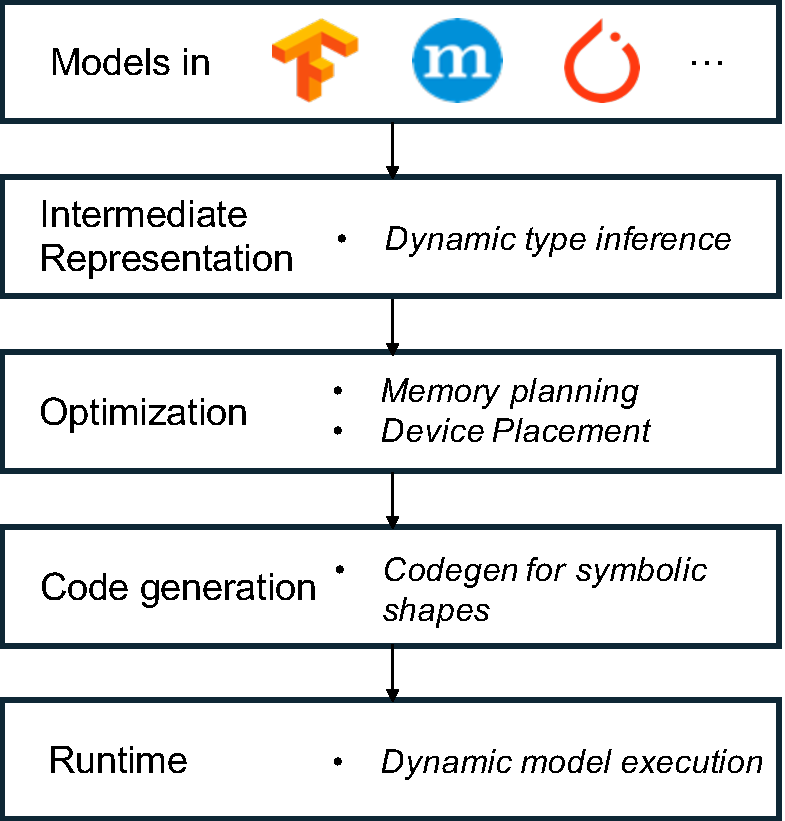
\includegraphics[width=.7\linewidth]{figs/dlc.pdf}
%   \captionof{figure}{
%   %\protect\yida{Can delete this figure if running out of space.}
%   A generic deep learning compiler workflow in multiple stages. Existing deep learning compilers are unable to process dynamic models due to lacking of the functionalities listed in each stage.}
%   \label{fig:dlc}
% \end{figure}

However, current deep learning compilers are not able to process dynamic models due to missing the following dynamism-specific features.% in the \emph{type system}, \emph{codegen}, and \emph{runtime}, along with dynamism-oriented optimizations such as \emph{memory planning} and \textit{heterogeneous device placement}.

\begin{itemize}
\item \textbf{An IR for representing dynamism.} Performing data type and shape inference on static models is straightforward as both the data type and shape of each operator are known during declaration and remain unchanged during runtime. However, the shape of an input tensor may vary wildly across different input samples in a dynamic model. The emergence of control flow constructs further complicates this problem as different execution paths can emit substantially different data. A fully static IR, hence, is inadequate to cope with the dynamic characteristics of these models.

\item \textbf{A set of dynamic-oriented optimizations.} Existing deep learning compilers, e.g. TVM \citep{tvm_osdi18} and Glow \citep{glow}, expect static input for each optimization. The memory size of each tensor is pre-allocated and their live cycles are determined using a dedicated optimization pass. They also ensure the homogeneous execution of the entire model because all kernels are executed on the same device with no data transfer between the host and device after a kernel is launched. However, these optimizations may completely break when dynamism appears. Now different execution path possibly requires different amount of memory and the sizes are not available before runtime. Certain simple IR nodes may also be introduced to help runtime type inference and memory allocation. The operations in these nodes are intrinsically more CPU friendly, which would lead to the serious performance problem if not placed on the correct device.

\item \textbf{A symbolic kernel code generator.}
Code generation (codegen) is responsible for generating high-performance executable kernels for operators. Recent research \citep{tvm_osdi18, glow, chen2018learning, zheng2020flextensor, adams2019learning} has achieved impressive results in kernel performance with static shapes on multiple backends.
Nonetheless, challenges in codegen with symbolic shapes remain unexplored.
After applying the same set of loop optimization, kernels generated with symbolic shapes could still perform bad if the loop boundary is not handled properly.
Meanwhile, kernel tuning under symbolic shape settings become more challenging as the search space grows exponentially.

%\yida{@Haichen, please revise this part accordingly. I feel that we should talk about about symbolic. And perhaps make it shorter, comparable with the other two points}
% The same operator (e.g. convolution) with different data shapes may require different kernels with different execution schedules to obtain preferable performance. There is no ``one-size-fits-all'' kernel and/or schedule that delivers consistently ``the-best'' performance across invocations with vastly different data shapes in a dynamic model. Instead, it requires the code generator to take the varied shapes into consideration and possibly generate a family of specialized kernels to maximize the performance of a dynamic operation. In addition, some common operators are well-optimized on specific platforms (e.g. MKL-DNN for Intel CPU and CuBlas for Nvidia GPU), and the code generator should be able to select kernels from third-party libraries if they will achieve the best end-to-end performance.

\item \textbf{A light-weight and cross-platform runtime.} For efficiency purpose, the runtime of static models could be simply designed a sequential executor that traverses the input data flow graph in the topological order and invokes operators sequentially. However, the execution path of dynamic models can only be determined at runtime and the kernels for certain operators must be dispatched according to the data shape determined at runtime, making a simple graph-style runtime insufficient.
\end{itemize}

Figure~\ref{fig:dlc} summarizes a generic deep learning compiler workflow in multiple stages, with the missing parts to supporting dynamism listed in each stage.  %\zhicomment{Figure needs to be updated, add heterogeneous device placement to optimization}.

\section{System Overview}
\label{sec:Relay-overview}

% \begin{figure}[t]
%   \centering
%   \includegraphics[width=\linewidth]{figs/Relay.pdf}
%   \captionof{figure}{Relay overview. Relay consists of a compiler that handles model with dynamism and a runtime that executes dynamic models in multiple platforms. Both components have multiple modules, which will be introduced in detail in the corresponding sections.}
%   \label{fig:vm}
% \end{figure}

After reviewing systems for dynamic deep learning models, this section gives an overview of Relay, a high-performance and flexible system for compiling and optimizing dynamic models for multiple platforms. In general, the design goals of Relay are:
\begin{enumerate}[leftmargin=*]
    \itemsep 0em
    \item {\bf Supporting dynamic models.} Relay targets models with all types of dynamism, including control flow, dynamic data structures and varied data shapes.
    \item {\bf Being portable and light-weight.} The module that Relay produces should be executable across a number of platforms on the cloud (high-end CPUs and GPUs) and at the edge (low-power CPUs and GPUs). The runtime should be light enough to run on devices with minimal compute power and memory capacity.
    \item {\bf Enabling high performance.} Relay should be performant in the context of dynamism across platforms.
\end{enumerate}

Figure~\ref{fig:vm} shows the system architecture of Relay that we propose to achieve the aforementioned design goals.
It is a system consisting of two major components, namely a compiler and a runtime.
Relay takes a model in the format of mainstream deep learning frameworks, converts it into a unified intermediate representation (\textit{IR}), then optimizes and compiles the IR into an executable that contains both platform-agnostic bytecode and platform-dependent kernel code, and finally loads the executable to execute in the VM-based runtime.
%\yida{The VM high-level description may be moved to the next paragraph, after compiler high-level description.}
%The bytecode is designed to only express the semantics of the IR, e.g. the control-flow and platform-dependent kernel invocation, through dedicated instructions, which contributes a negligible portion of the total execution time, as we will show in~\autoref{sec:eval}.
The bytecode is executed by Relay's runtime interpreter, which is shareable across various platforms.
This design effectively enables us to only maintain one version of the execution logic, but focus more on the performance critical operator kernels.
The kernels are highly-optimized for a specific hardware platform to achieve high performance.
%Kernels optimized for data with different shapes are compiled separately and dispatched accordingly.

To effectively support dynamic models without performance degradation for static models, we introduced various analysis and optimization techniques in Relay's compiler.
First, a set of IR extensions are devised to represent dynamic shapes (\textit{Any} shape) and dynamic allocations for static optimization of dynamic program behaviors (\autoref{sec:compliation:typing}).
Second, shape functions are attached to operators to compute the output shapes dynamically and perform type checking at runtime (\autoref{sec:compilation:shape-func}).
Third, a memory planning optimization is employed to reduce amount of memory consumed (\autoref{sec:compliation:memory}).
Fourth, a heterogeneous device placement mechanism is designed to place IR nodes on ``the-best'' device to reduce expensive cross-device data transferring and synchronization (\autoref{sec:compliation:hetero}).
Finally, the compiler features a code generator that is capable of specializing the code generation of certain likely shapes (\autoref{sec:compliation:codegen}). Once the executable with dynamic behavior is compiled, the VM-based runtime can load and interpret it with intelligent dynamic kernel dispatching (\autoref{sec:runtime}). We detail the design and implementation of each of these features in the followed sections.

\section{Compiler Support for Dynamism}
\label{sec:Relay-compliation}

A key challenge preventing existing deep learning compilers from handling dynamism is the lack of a uniform and dynamic representation. For example, optimizations and runtime of existing IR, e.g. TVM \citep{tvm_osdi18}, assume the presence of static shape information in numerous places. These assumptions are present in many other so-called graph compilers and introduce quite a few challenges for optimization.

In order to handle dynamism, we design a set of IR extensions which expose the essential semantics required to optimize dynamic programs. The approach is implemented in Relay on top of the Apache TVM (version 0.6) deep learning compiler infrastructure \citep{tvm_osdi18} to leverage its frontend converters from various DL frameworks to its IR. TVM's frontends alleviate the need to frontend specific details enabling our work to focus on contributions such as IR extensions and optmizations. To use Relay, one only needs to feed it with a pre-trained model, perform compilation and then inference. Furthermore, the lessons
here are applicable to other compiler efforts such as TensorFlow's MLIR support or PyTorch's TorchScript and TensorExpr (a Halide and TVM inspired DSL for kernel codegen) work. The below section
describes how we transform standard TVM programs into a our dynamic dialect which enables us to easily apply static optimizations to dynamic programs, much as we do in traditional compiler optimization.

In this section, we detail three key components required to compile dynamic models.

\begin{itemize}
    \item An extended type system which enables statically tracking dynamic shapes.
    \item A series of optimization passes that make dynamic output shapes, allocation, and device placement explicit.
    \item A set of codegen techniques for producing code for kernels with dynamic input and output shapes.
\end{itemize}

\subsection{Typing}
\label{sec:compliation:typing}
Deep learning compilers use type systems to represent, check and infer the data types and shapes of tensors. In some frameworks and compilers this is separated into two steps, shape inference and data type inference. TVM~\citep{roesch2019relay} performs both simultaneously and refer to them as type inference, terminology we will use throughout the section.

A {\em Tensor Type} is designated by an $n$-dimensional shape (defined as a tuple of integers describing the tensor's dimensions) and a data type (e.g. \texttt{float32} or \texttt{int64}).
Current deep learning IRs only support codegen when all dimensions of a tensor's shape are known at compile-time.
Static shapes are mandatory for type inference and checking in existing deep learning compilers.

In the context of dynamic models, many data shapes can only be determined at runtime. Therefore, the previous assumption of static data shapes does not hold.
In order to support dynamic data shapes, Relay introduces a special dimension called Any~to represent statically unknown dimensions.
For example, we can represent a tensor type as \texttt{Tensor[(1, 10, Any), float32]},
where the size of the third dimension in this tensor is unknown while the other
two dimensions have concrete values.
This concept is relatively uncontroversial, and has been introduced in other frameworks.
Janus \citep{jeong2019janus} uses similar denotation to represent a dynamic dimension but only for type unification, while Relay extends type inference to handle Any~as described next. We do not support tensor types with dynamic ranks given the relatively limited use cases and optimization opportunities.
%\yida{Do we need the following sentence?}The challenge of introducing a dynamic shape extension is adapting each layer of the system to handle it in a way that does not greatly degrade performance.

\noindent
{\bf Operator Type Relation} A type relation describes the relationship between the types of operator inputs and outputs. The type system of TVM's Relay IR relies on these type relations to infer and bidirectionally propagate type and shape relationships between inputs and outputs of operators across the whole program.
For example, the type relation for broadcasting operators (e.g. \texttt{broadcast\_add}) performs the shape calculation following the NumPy broadcasting rules\footnote{\url{https://docs.scipy.org/doc/numpy/user/basics.broadcasting.html}}.

The type relation must be generalized to properly handle dynamic shapes. For example, a program which grows a tensor on each loop iteration (a case existing in the decoder of many NLP models) is both impossible to type and compile without proper type system support. With the introduction of Any, we are able to improve the existing type relations to support dynamic models.

There are two cases that must be handled after we introduce Any~to the type relations.
First, operators such as {\tt arange}\footnote{{\tt arange} generates a range of values in a (start, stop, step) interval the arrays output size is a function of input arguments.} and {\tt unique}\footnote{{\tt unique} selects the unique elements of a tensor.} have dynamic output shapes depending on the input data, which will be described in Any.
% We can now describe the type relation using the enhanced type relation functions with Any but not before.
% For example, type relation of {\tt arange} can be expressed as follows
% \[
% arange: fn(start: fp32, stop: fp32, step: fp32) \rightarrow \langle [Any], fp32 \rangle
% \]
Second, when input shapes of a type relation contain Any~dimension, the type relation needs to propagate Any~correctly to the output types and relax typing constraints that hold in the static cases when necessary.
%For example, type relation for {\tt broadcasting} operators determines the compatibility between corresponding dimensions from both inputs if they are equal or one of them is 1 according to the Numpy broadcasting rule.
For example, the rules
for broadcast type relation given the matching dimension from two inputs when having Any~are defined as follows:
\begin{align*}
  \textrm{broadcast\_rel}(Any, 1) &\rightarrow Any \\
  \textrm{broadcast\_rel}(Any, d) &\rightarrow d ~~~~~~(d > 1) \\
  \textrm{broadcast\_rel}(Any, Any) &\rightarrow Any.
\end{align*}
Note that due the presence of dynamic shapes these type relation rules can no longer rule out all type errors at compile-time.
For example, for the second rule shown above, when Any~is neither 1 nor $d$ at runtime, it then violates the broadcast type constraints.
To address this, we take the gradual typing~\citep{gradualtyping} approach and leave certain type checking at runtime after Any~is instantiated by a
concrete value (see \autoref{sec:compilation:shape-func} for more details).
One could eliminate these errors using a more advanced type system, but at increased complexity.

\noindent
{\bf Type Inference} One caveat of the Any~dimension is that unknown dimensions will propagate during type inference, reducing chances for shape specialization.
For example, if we use an operator such as {\tt arange} to produce a tensor with dynamic shape (i.e., \texttt{Tensor[(Any,), f32]}) and later {\tt broadcast\_add} to a tensor with static shape (i.e., \texttt{Tensor[(5, 1), f32]}), the output shape will also contain an Any~dimension (i.e., \texttt{Tensor[(5, Any), f32])}.

To limit the contamination of Any, we further introduce {\em sub-shaping} to improve the precision of types computed by type-inference.
Much like sub-typing used in popular programming languages \citep{LiskovTPLS1994,AmadioAmadioTPLS1993}, our extension enables values with more specific shape information to be passed in contexts which require less specific shapes.
Further, we perform extra analysis on each Any~dimension to detect if two Any~dimensions point to an identically sized dimension. We can use this analysis in the downstream compilation to generate shape-specialized code during codegen.
% We treat concrete dimension and symbolic dimension as a sub-shape of Any.
% \yida{The following sentence is problematic with grammatical error. We need to explicitly define what is an argument.}Rules for invoking a function, suppose fn type is $fn\langle T_1, \dots, T_n\rangle$,
% and arguments are $T'_1, \dots, T'_n$, the rules are defined as follows
% \begin{align*}
%   \textrm{union}(T_i, T'_i) &\rightarrow T_i \\
%   \textrm{join}(T_i, T'_i) &\rightarrow T'_i
% \end{align*}

\subsection{Shape Function}
\label{sec:compilation:shape-func}
%Existing deep learning compilers only deal with static shapes, enabling all shape computation to occur at compile-time.
%Therefore, it is easy to allocate memory for the tensors using static shape information to compute the precise amount of storage needed for each tensor.
%However, introducing Any~invalidates this pre-allocation mechanism as the tensors may now contain dynamic dimensions.
The introduction of Any~dimension invalidates the pre-allocation mechanism adopted in the existing deep learning compiler.
Instead, we now have to track the amount of memory required to be allocated in parallel to computing.
Furthermore, static type checking cannot eliminate all type errors at compile-time due to dynamic tensor shapes.
Consequently, we define a {\em shape function} to compute the output shape for storage allocation and verify the type relation in accord with the semantics of every operators.
The shape function is similar in structure to the type relations described in \autoref{sec:compliation:typing} but are present at runtime instead of compile-time.
The shape function enables compiling and embedding the computation of output shapes into the program.

According to the characteristics of the operator, we divide the shape functions in three different modes: data independent, data dependent, and upper bound.
{\em Data independent} shape functions are used for operators in which the output shape only depends on the shapes of inputs such as normal 2-D convolution.
{\em Data dependent} shape functions require the concrete input values to compute the output shapes. For example, the output shape of \texttt{arange} depends on the value of start, stop, and step.
In addition, there are certain operators such as Non Maximum Suppression (\texttt{nms}) where the complexity of computing the output shapes is on par with the complexity of executing the operator itself.
In order to avoid the redundant computation, we use an {\em upper bound} shape function to quickly estimate an upper bound shape for the output.
We also require such operators to return the output shape along with output value, so as to use the real shape to slice the output tensors into precise output shape and layout.

It is worth noting that in the presence of dynamic shape functions, operator fusion needs to be specially taken care of.
Operator fusion, which combines {\em basic operators} into a {\em composite operator}, is a critical technique for performance optimization as it reduces unnecessary memory copies and improves the cache locality.
%However, we only define the shape function at elementary operator level. As a result, we also must fuse shape functions in parallel with the operator fusion.
The compiler can easily connect the shape functions of basic operators to form the shape function for a composite operator when all shape functions are data independent.
However, a basic operator with a data dependent or upper bound shape function cannot be fused to other operators, i.e., taking the outputs of other operators as its inputs to fuse together, as the shape function requires to access to the intermediate result within a composite operator.
As a result, we explicitly define the fusion policy to prevent this from happening.
%If all basic ops in a composite op have data independent shape functions, it is straightforward to generate shape function for this composite op as we can just connect the shape functions of basic ops together. However, a composite op is invalid if a basic op that has a data dependent or upper bound shape function takes the intermediate output of another basic op as input.
%Because the intermediate result in a composite op is inaccessible from outside, the data dependent shape function cannot collect all arguments it required. Thus, we revise the operator fusion policy correspondingly to make sure composite ops generated by the operator fusion pass will be valid.

%Due to our definition of shape functions we are able to perform fusion using a generalized version of the algorithm used for standard operator fusion which handles passing the appropriate input shape or input depending on the shape function. For example imagine that the fuse operator has a single input that was originally used an operator that requires the input, and the second fused operator requires the input shape. Depending on the type of the shape function defined above, we handle operator fusion in the following manner. Any data independent shape functions could be fused with other operators. Any fused group can only have at most one shape function and it should be fused together with the operator that needs shape function.

\subsection{Memory Planning}
\label{sec:compliation:memory}
Deep learning workloads are dominated by two key aspects, compute-intensive kernels and memory allocation. Many deep learning compilers use a form of static memory planning which tries to coalesce memory and minimize allocations. For devices such as GPUs these optimizations are essential for reducing memory fragmentation and ensuring allocation does not hamper kernel performance. Existing deep learning compiler IRs hide memory allocation behind a functional interface, where each operator implicitly allocates their output storage. Then before execution, the system performs static-memory planning on the data-flow graph enabling efficient pre-allocation of the required memory. Due to this ``out-of-band'' nature of memory allocation, it is challenging to customize, modify or compose memory optimizations with other passes. For example, if one needs to adjust memory allocation for heterogeneous execution, modifications to the runtime are required.

Alternatively, some systems lower the entire program to low-level IRs such as LLVM~\citep{llvm} in order to perform optimizations. Due to the coarse-grained memory semantics of deep learning models, it is essential that memory optimizations occur at a suitably high-level of abstraction before essential program facts are lost. Moreover, as discussed in~\autoref{sec:compilation:shape-func}, we have introduced new ways to account for the handling of dynamic allocations, which further complicate memory analysis.
In order to perform dynamic memory planning we have extended TVM's Relay IR, using these extensions we translate a IR dialect where all memory allocations are implicit to one where buffers are allocated and passed around explicitly. The key to this transformation is an inter-procedural change of calling convention, with each operator now taking its outputs explicitly it is possible to track and transform allocations.
In particular, we have introduced four new IR constructs, (a) \verb|invoke_mut(op, inputs, outputs)| which takes outputs as mutable in-out arguments, (b) \texttt{alloc\_storage(size, alignment, device)} which allocates a region of memory of a particular size, (c) \texttt{alloc\_tensor(storage, offset, shape, dtype, attrs)} which allocates a tensor at a particular strorage offset with a shape and data type, and (d) \verb|kill(tensor)| which frees a tensor before its reference count becomes zero due to exiting the frame. Note that in the below code examples \texttt{Tensor<d1, ..., dn>} is shorthand for a tensor of shape \texttt{(d1, ..., dn)} containing floating point values.

We can demonstrate how to transform a single statically shaped operation such as broadcasting addition.

%\begin{Verbatim}[fontsize=\small]
\begin{lstlisting}
fn main() -> Tensor<10> {
  let t1, t2 : Tensor<10> = ...;
  add(t1, t2)
}
\end{lstlisting}
%\end{Verbatim}

Here we only must allocate a single buffer, the return buffer for the addition operation.

%\begin{Verbatim}[fontsize=\small]
\begin{lstlisting}
fn main() -> Tensor<10> {
  let t1 = ...; let t2 = ...;
  let storage = alloc_storage(40, 64, cpu(0));
  let out1= alloc_tensor(storage, 0, (10), f32);
  invoke_mut(add, (t1, t2), (out1));
  out1
}
\end{lstlisting}
%\end{Verbatim}

The above transformation replaces all operator invocations with a call to \verb|invoke_mut| allocating storage
for backing a single tensor from allocated at offset zero.
The key insight is to internalize a notion of memory allocation into the IR, enabling static optimization of
both static and dynamic allocations presence of control and dynamic shapes. We realize our shape functions as fragments of TVM's tensor expression language which computes the output shape for a particular operator. As detailed in~\autoref{sec:compilation:shape-func} our shape functions may require the input, the input \textit{shape}, or both.
Our uniform treatment of shape functions as standard tensor expressions enables them to be fused and optimized like normal, but one challenge is that we must now manifest allocations in a fixed point until we allocate for both the compute and necessary shape functions. We illustrate this below with a single dynamic concatenation.

%\begin{Verbatim}[fontsize=\small]
\begin{lstlisting}
fn (x: Tensor<?,2>, y: Tensor<1,2>)->Tensor<?,2> {
  concat((%x, %y))
}
\end{lstlisting}
%\end{Verbatim}

This is the same transformation as the previous example with the addition of carefully inserting
invocations to the shape function to compute output buffers sizes for the dynamically sized kernel.

%\begin{Verbatim}[fontsize=\small]
\begin{lstlisting}
fn (x: Tensor<?,2>, y: Tensor<1,2>)->Tensor<?,2> {
  let in_sh0 = shape_of(x);
  let in_sh1 = shape_of(y);
  let storage_0 = alloc_storage(16, 64, ...);
  let out_sh0 = alloc_tensor(storage_0, ...);
  invoke_shape_func(concat,
      (in_sh0, in_sh1), (out_sh0,), ...);
  let storage_01 = alloc_storage(...);
  let out_0 = alloc_tensor(
      storage_01, shape_func_out_0, ...);
  invoke_mut(concat, (x, y), (out_0));
  out_0
}
\end{lstlisting}
%\end{Verbatim}

After the transformation you may notice we have introduced calls to \verb|shape_func| which invokes a shape function for a kernel. The shape function requires input shapes as arguments which further require us to invoke \verb|shape_of| for both \verb|%x| and \verb|%y|. \verb|shape_of| will be directly mapped to a VM instruction to retrieve the shape of a tensor at runtime. More description of it will be provided in \autoref{sec:compliation:hetero}.

Now that the all allocations are explicit in the IR we can provide analogous optimizations in the static
case on dynamic programs, for example we have implemented a storage coalescing pass which groups storage
into a larger region which we can then multiplex tensor allocations on to.


\subsection{Heterogeneous Device Placement}
\label{sec:compliation:hetero}
As discussed in Section \autoref{sec:compilation:shape-func}, shape functions are executed at runtime to calculate the output shape of an operator. These functions must execute on the CPU due to the host-interaction model of GPU like devices. In the case of heterogeneous execution (i.e., CPU and GPU) it is essential to carefully schedule the execution of shape functions and kernels as improper scheduling can be disastrous for performance. For instance, considerable overhead will occur if inputs to shape functions must be copied from GPU due to the cost of data transfers and synchronization. To minimize the performance penalty, we analyze the program allocations to place sub-expressions on the most suitable devices.

We introduce a unification based analysis for computing the correct device placement and allocation based on the previous scheduling of the compute kernels. The goal of our device analysis is assigning each IR node in a way that minimizes the number of cross-device copies. We introduce a concept of \texttt{DeviceDomain} to represent the domain of a device, including source and destination. Each expression in the IR defaults to the empty domain, meaning there are no constraints on its device placement. In addition, two new IR constructs are introduced to facilitate the heterogeneous execution of VM, namely \verb|device_copy| and \verb|shape_of|. The former performs a data transfer between different devices and is inserted when a cross-device data copy is mandatory. The latter is used to retrieve the shape of a tensor at runtime and is used to efficiently compute the input shapes for shape functions. Our analysis is formulated as a set of device placement rules which describe how device constraints flow, and then we use unification, a technique common in type inference and compilers in order to compute precise device placement.

\begin{itemize}
    \item \verb|shape_of|. Defaults to the CPU domain because we can access a Tensor's shape regardless of which device it is placed on.
    \item Shape functions. These IRs take the output of one or multiple \verb|shape_of| and then derive the shape of an operation according to predefined type inference rules. The output of a shape function is used to compute the amount of memory that this operator requires at runtime, which only needs a few cheap scalar arithmetic computation. Therefore, the inputs and outputs would be better on a CPU domain as well.
    \item \verb|device_copy|. The input and output of this IR are on different domains as it copies data from one domain to another. The device domains of the input and output are propagated in the opposite directions to other IR nodes that are reachable to/from the device copy node.
    \item Memory operations. The device domain of storage from \verb|alloc_storage| is designated in the expression, and later is propagated to the device domain of the tensors allocated from this storage via \verb|alloc_tensor|.
    %in the instruction computation of the allocation size and the shape for memory operations, such as \verb|alloc_storage| and \verb|alloc_tensor|, should be on CPU due to low computation intensity.
    \item \verb|invoke_mut|. All arguments used in the \verb|invoke_mut| must have the same device domain.
    \item Other common IR nodes. The device domain of other common IR nodes, e.g. variables, constants, operators, etc., can be directly propagated from the above nodes.
\end{itemize}

Based on the rules defined above, we use a union-find data structure to bidirectionally propagate and unify the device placement of each IR node. We introduce two operations, \texttt{union(s, t)} and \texttt{find(s)}, to achieve \texttt{DeviceDomain} unification throughout the entire program. \texttt{union(s,t)} unions the equivalence device domains of \texttt{s} and \texttt{t} into one equivalence domain when the device types match. \texttt{find(s)} returns the representative of the device domain that \texttt{s} belongs to. These two operations are applied until all IR nodes are annotated. The result of the heterogeneous device placement composes with memory planning and shape function insertion resulting in correctly placed allocations.

\subsection{Symbolic Codegen}
\label{sec:compliation:codegen}
%\yida{Should we mention the mechanism of invoking third-party libraries in this subsection?}
Deep learning compilers~\citep{tvm_osdi18, halide} have demonstrated competitive performance compared to manually tuned kernels on multiple platforms. Recent trends apply machine learning based search to further reduce or eliminate complex manual performance tuning, existing work applies both template based~\citep{chen2018learning, zheng2020flextensor} and beam search based~\citep{adams2019learning} ones.

However existing work which focuses on tuning in the presence of static shapes falls short with symbolic or dynamic shapes. There are two inherent challenges with regard to codegen with symbolic shapes.
\begin{itemize}
    \itemsep 0em
    \item How to achieve the same performance of kernels generated with symbolic shapes as that with static shapes when applying the same schedule?
    \item How to extend the machine learning based approach to tune kernels with symbolic shapes?
\end{itemize}

Loop parallelism and loop tiling are common optimization techniques that exploit multi-core capabilities by achieving data access patterns which are memory hierarchy aware for both CPUs and GPUs. However, the combination of these techniques lead to complex loop boundary conditions. In many static cases, it is possible to prove these conditions always hold, and thus eliminate checks which hamper further optimizations such as unrolling.
While straightforward to handle with static shapes, it becomes a non-trivial challenge when performing symbolic codegen. If not carefully handled, the boundary condition checks will stay, leading to poor performance.

To address this issue, we generate multiple kernels according to the residues modulo of the tiling factor and then dispatch based on the actual shape at runtime.
For example, suppose a symbolic dimension $x$ is divided by a factor of 8, we then duplicate the generated kernel for 8 times, and replace the symbolic var $x$ by $8k+r$ in each copy, where $k = \lfloor x / 8 \rfloor$ and $r \in [0..7]$. By applying this technique in conjunction with an enhanced symbolic expression simplification pass, we can eliminate most boundary checks to achieve performance that is nearly identical to kernels compiled with a single static shape. Lastly, we automatically generate a dispatch function that invokes the corresponding kernel based on the residue.
%because this function is also generated in the IR we can compile and optimize it like other code ahead of time.
In addition, the dispatch function can be extended to invoke either compiler generated kernels or third party library whichever is faster from the profiling results.
The increased kernel size is relatively small compared to the overall deep learning models.
In extreme cases where resources are extremely limited, we can either generate fewer number of kernels than the tiling factor or reduce the tiling factor to find an acceptable trade-off between code size and performance.

A known issue to machine learning based tuning is that it may take a long time (usually hours) to find the best schedule for a single kernel. When it comes to symbolic shapes, the tuning time may be exponentially longer if we naively tune for every possible shape. In this paper, we extend the template based tuning approach for symbolic shapes in order to make tuning time tractable. The template based tuning approach takes a human-defined code template and a search space, and searches the best configure within the search space by using machine learning algorithms.
%by building on the techniques explored in based~\citep{chen2018learning}.
We observe that a good configuration for one shape usually performs well on other shapes. Based on this observation, we devise the following mechanism to tune the kernel for symbolic shapes.

\begin{enumerate}[leftmargin=*]
    \itemsep 0em
    \item First replace the symbolic dimensions by a large enough value (e.g., 64) such that the search space can cover most possibilities, and run the tuning algorithm on the static shape for a sufficient number of iterations.
    \item Pick top $k$ configurations, apply them to a selection of other shapes, and evaluate their performance.
    \item Pick the configuration that performs best on average among shapes previously evaluated.
\end{enumerate}

We found that $k=100$ covers most of the best configurations for other shapes. Current popular dynamic models usually only require kernels with one symbolic variable. As a result, we choose the values of power of two up to 256 in the cross evaluation of other shapes. If there is more than one symbolic variable, a more sophisticated selection approach might be required to limit the evaluation time of step 2. We leave this to the future work. Further, if the workload distribution is known, we could adjust the weighting of known shapes when picking the best configuration for step 3.

Though we address both challenges, we admit that our approach has limitations when all dimensions are unknown. In these cases symbolic codegen cannot completely replace manually tuned 3rd party libraries yet, but is complimentary when partial shapes are known.

% Our codegen approach for dynamic shapes is designed to integrate well with TVM's codegen. We implement a bucketing
% based codegen strategy, which generates a set of shape-specialized variants and code which selects between them. One
% attractive consequence of this design is that it allows us to integrates with the current version of AutoTVM~\citep{chen2018learning}, TVM's auto-tuning framework
% to further optimize kernels.

% When an operator appears with dynamic shape it often will only vary along a single dimension. We are able to handle cases that
% deal with imperfect tiling strategies but the critical performance piece is choosing a tuned operator with the appropriate tile size.
% We reuse the machinery of the VM to support invoking a bucketed operator. For each operator with a dynamic shape we will
% generate tile sizes for powers of two, and then for a given input size round to the nearest power of two tile size and select that operation.
% The code for selecting between buckets is also realized as TVM expression allowing further optimization of the combined kernel.
% This strategy can be viewed as a form of polymorphic inline caching~\citep{inline_caches}, where the cache is not keyed by type, but shape.

% The bucketing strategy we employ obtains
% For this paper we explored one possible strategy for generating code but using the infrastructure of this paper
% it is relatively low cost to explore new strategies by reusing the machinery.


\section{Virtual Machine}
\label{sec:runtime}
The conventional runtime of existing deep learning compilers which naively executes a model node by node in topological order does not work for executing the compiled modules of dynamic models. A more intelligent and powerful execute engine is required to handle the control flow execution logic, and dispatch different kernels accordingly. In order to achieve these goals and be portable to different platforms, we design and implement a virtual machine (VM)-based runtime.

In Relay, we compile a dynamic model into a {\em VM executable} that contains platform-independent bytecode and platform-dependent kernel code, which can be later loaded and executed.
The bytecode consists of a series of instructions that predicate the order of kernel invocation and control flow execution logic.
This design compliments conventional runtime's capability for executing highly optimized kernels but not directly handling orchestration between kernels.
%The VM compiler lowers dynamic models to VM instructions, while kernels are lowered to native code via our modified version of TVM.

\subsection{VM ISA}

%The implementation of the VM compiler is straightforward, with the interesting design decisions found in our instruction set's design.
The design of the VM instruction set is motivated by the simple observation that kernel execution dominates neural network execution time. If we treat kernel invocation as a single instruction, the cost of surrounding instructions is negligible in the total execution.

As a result, our design is quite different from traditional language virtual machines, which contain many instructions that perform little work, leading to a profile where the cost of each instruction executed matters.
Our ISA is composed of CISC-style instructions in which each instruction corresponds to a primitive IR expression on tensors, such as allocation and kernel invocation, which in turn may correspond to executing multiple ``low-level'' operations. For example, \texttt{LoadConst idx, \$reg} is capable of multiple addressing modes as it first reads the index \texttt{idx} and then loads the data from a constant pool to the destination register \texttt{\$reg}.
A complete list of instruction set can be found in the appendices.
We naturally select a register-based virtual machine design~\citep{davis2003case} for compact a bytecode, which is easy for users to read and modify. We provide the abstraction of an infinite set of virtual registers as it significantly simplifies optimizations and allocation (similar to SSA) and minimizes conceptual barriers to rapid prototyping and modification.

Instructions are represented using a traditional tagged union containing the op-code and the data payload. This representation enables both efficient serialization and instruction decoding and dispatch. Relay uses variable-length instruction format due to the inclusion of variable sized operands such as data shapes in the instructions.

\begin{comment}
\begin{table*}[t]
\centering
\small
\input{figs/table_isa}
\caption{The opcode and the description of the Relay instruction set \label{tab:isa}}
\end{table*}
\end{comment}

% This design has the following benefits. First, both CISC instructions and variable length encoding contribute to better code density. This is a significant advantage for edge devices that only have limited resources. Second, allowing multiple addressing modes to execute a single instruction can reduce the amount of data fetched from cache hierarchy and main memory. It may also lead to better spatial locality as the data (e.g. the tensor value) may remain in the cache. Third, a variable-length instruction encoding paves the way for extending extra information to instructions, e.g. debugging and even branch prediction. Last but not least, the instruction designed in Relay effectively separates hardware-dependent kernels from model control logic. The Relay bytecode is hardware-independent which eases bytecode serialization, and can be paired with hardware-dependent kernels being invoked by the \texttt{InvokePacked} instruction.

\subsection{Interpreter}

After we have generated a VM executable,
%\yida{we never define what is a VM executable}
we can create an interpreter by loading the executable. When execution begins, the interpreter runs a dispatch loop which checks the op-code and executes the appropriate logic, then repeats. As our instructions are coarse-grained (i.e. they can be viewed as super-instructions), the number of branches generated by the dispatch-loop is lower than traditional programming language VMs, adding negligible overhead compared to ahead of time compilation.

VM uses a tagged object representation reminiscent of those used by programming languages such as Haskell, and OCaml. The tagged object representation smoothly integrates with various data structures, including tensors, algebraic data types, and closures. Due to the specialized object representation, VM instructions only need to interact with the coarse-grained data (i.e. tensors) requiring infrequent memory allocation in chunks.

In sum, the interpreter handles instructions in the following categories.
%\yida{somewhat mention interpreter in the above two paragraphs, otherwise it feels disconnected}

\begin{itemize}[leftmargin=*]
    \item Register-to-Register Operations. Register-to-Register operations, e.g. \texttt{Move}, transfers data between different offset of the register file. Objects are reference counted, make use of copy-on-write and passed by reference ensuring register operations are cheap even if the size of underlying container is large.

    \item Memory Operations. Memory operations can allocate space for tensors, load constant tensors, and so on. Due the design of our constant pool, weights (which are constant during inference) can remain in-memory with no specialized support they can be referenced by the\texttt{LoadConst} instruction.

    \item Call Operations. Call operations are the most frequently executed instructions. The ISA
    has specialized call instructions for invoking a global function, a kernel primitive, closure, copying data across devices, reshaping runtime tensors, and calculating the shape of tensors. Kernel primitives are ahead-of-time compiled through and can leverage both compiler-generated kernels and the third-party libraries.
    %\yida{Should we briefly mention how to decide which kernels (in the context of multiple kernels) to invoke? I don't mean whether to invoke compiler-generated kernels or third-party libraries.}

    \item Control Flow Operations. Unconditional jump instructions, e.g. \texttt{ret}, are used by both static and dynamic models to jump to a specific program point. Only dynamic models need conditional control operations to determine the direction of branching. The interpreter updates the PC using the offset from either the true branch or false branch based on the conditional value.
\end{itemize}

\begin{comment}
\lstset { %
    language=C++,
    basicstyle=\ttfamily\footnotesize,% basic font setting
    keywordstyle=\bfseries\color{green!40!black},
    commentstyle=\itshape\color{purple!40!black},
    stringstyle=\color{orange},
}
\begin{figure}[htbp]
\centering
\begin{lstlisting}
void RunLoop() {
  this->pc = 0;
  Index frame_start = frames.size();
  while (true) {
  main_loop:
    auto const& instr = this->code[this->pc];
    switch (instr.op) {
      case Opcode::LoadConst: {
        auto constant_obj = constants[instr.kidx];
        // ...
        RegWrite(instr.dst, const_pool_[instr.kidx]);
        pc++;
        goto main_loop;
      }
      case Opcode::Invoke: {
        // Prepare args and then invoke.
        InvokeGlobal(functions[instr.func_idx], args);
        frames.back().caller_ret_reg = instr.dst;
        goto main_loop;
      }
      case Opcode::InvokePacked: {
        // Invoke primitive functions
        const auto& func = packed_funcs[instr.pidx];
        const auto& arity = instr.arity;
        // Read args from the register file.
        InvokePacked(instr.pidx, func, arity,
                     instr.osize, args);
        // Write outputs to the register file.
        pc++;
        goto main_loop;
      }
      // Other opcodes are omitted
    }
  }
}
\end{lstlisting}
\caption{Relay bytecode interpreter.}
\label{fig:interpreter}
\end{figure}
\end{comment}

\subsection{Discussion}

%\haichen{compare against AOT. discuss other use cases for vm, e.g., resource isolation, security, integration into a larger system}

%The VM can be seen as the realization of a tensor abstraction machine, which corresponds to high-level tensor operations such as allocating a tensor, invoking an operation like conv2d, or performing a device copy.
An alternative solution to the VM could be ahead of time compilation from our abstract machine into machine code.
But due to the granularity of the operations, dispatch time makes up a very small portion of the execution time. More importantly, the VM provides flexibility traditionally attributed to virtual machines and a clear compiler/runtime split.
We see the potential of VM to be integrated as a runtime module into a larger system.
For example, VM can provide resource isolation where multiple inference instances share the same hardware in the cloud. Furthermore, a Quality of Service (QoS)-aware system, e.g., \citep{kang2018hotmobile, Yachir2009rsj}, could leverage VM to pause the current model execution for a higher priority or time-critical model. Last, because of the simplicity of the VM design, one can verify the implementation of VM for security and privacy purposes.

%Our VM is designed to execute the dynamic models by removing the limitations of the existing runtimes which only support statically shaped programs.
%\yida{Mention the bytecode+kernel design. Also mention other potential use case of VM, like isolation?}

%\subsection{Kernel dispatcher}
%Op fusion across control flow, e.g., pushing ops into if/else branch for more fusion.

% we probably want to talk about this in the instruction set or memory planning. No need to have a separate paragraph here.
%The design of Relay focuses on the simplicity without sacrificing performance. In order to accomplish this, we design a tensor VM rather than a scalar VM. In the tensor VM setting, we optimize for cheap ``allocation'' of objects (by trying to avoid real allocation), reuse of static fragments, and the ability to support dynamic shape (i.e jagged tensors). \autoref{fig:vm} depicts the overview design of VM. It essentially contains a compiler and a runtime system. The compiler compiles a Relay program into both hardware dependent and hardware independent modules/libraries. The hardware independent code consists of low-level bytecode that is specifically designed for efficient execution of VM. The hardware dependent code is composed of coarse-grain operators registered in the TVM operator inventory (TOPI). The runtime system takes charge of the execution of generated bytecode, i.e. dispatching the instructions and managing the stack frame and registers. We will detail the design of the VM in the following sections.

%\zhicomment{@haichen,  Do you still need push and pop? I think we probably don't need them now, instead we use \textit{Move} to manage stack. Am I right?}
%\textit{stack-based} and \textit{register-based} virtual machines are the two major types of VM in programming languages. Stack-based VM aims at simplicity, using \textit{push} and \textit{pop} instructions to maintain a unified stack. However, it complicates tasks such as dataflow analysis and enforces certain orders in the execution. Instead, register-based VM design manages registers to designate the operands and results rather than the stack. This type of VM simplifies the calling convention as values are carried by registers. But it may bring some cost in terms of code size as it needs to decode instructions to fetch the values at specific positions. As aforementioned that our VM mainly targets tensor-level instructions instead of low-level machine instructions. The code size is thus generally small. Furthermore, we would emphasize the convenience of optimizations, such as liveness analysis and memory allocation in the model inference scenario. Therefore, the register-based VM provides more benefits which meets our selection.

\section{Evaluation}
\label{sec:eval}

This section evaluates the performance of Relay on dynamic models against existing state-of-the-art solutions, as well as discussing the role of the optimizations performed by Relay. Specifically, the section seeks to answer the following questions:
\begin{enumerate}
    \item What is the overall performance of Relay for dynamic models when compared against state-of-the-art alternatives on various hardware platforms?
    %\item How much overhead does Relay introduce for static models on top of the state-of-the-art solutions?
    \item How much overhead does Relay VM introduce for handling dynamism at runtime?
    \item How effective are the proposed optimization techniques, such as memory planning and symbolic codegen?
\end{enumerate}

%\yida{Evaluate the execution time of the bytecode as a portion of the total execution time, to show that VM overhead is negligible}
%\note{End-to-end: BERT, LSTM, Tree-LSTM on Intel CPU, ARM CPU, NVidia GPU; Relay-runtime vs. graph runtime. Optimization implication: Kernel dispatch or not; memory planning or not; number of dispatched kernels.}
\subsection{Experiment setup}
\label{sec:eval:setup}

All experiments were conducted on Amazon EC2 instances. We evaluated Relay on three hardware platforms: Intel Skylake CPUs (c5.9xlarge, 18 physical cores, hereinafter called {\em Intel CPU}), Nvidia Tesla T4 GPUs (g4dn.4xlarge, 1 card, 2,560 CUDA cores, hereinafter called {\em Nvidia GPU}), and ARM Cortex A72 (a1.4xlarge, 16 physical cores, hereinafter called {\em ARM CPU}). Although all tests are done on the cloud, our results of ARM CPU are portable to the edge devices, e.g. Raspberry Pi, due to the same architecture. %All cores have uniform memory access.

To study the efficiency of Relay in handling dynamic models, we compared it with mainstream deep learning frameworks, including TensorFlow (v1.15), MXNet (v1.6), PyTorch (v1.5) \footnotemark, as well as dynamic-specific systems TensorFlow Fold based on TensorFlow v1.0.
\footnotetext{We use PyTorch v1.4 on ARM CPU because PyTorch v1.5 fails to build on ARM instance.}
%For TensorFlow Fold, its execution latency would include the compilation time (\zhicomment{@haichen, we probably need a bit argument here for why compile time is included.}).
We were unable to compare Relay with Cavs~\citep{xu2018cavs}, JANUS~\citep{jeong2019janus}, or Jeong et al.\citep{jeong2018improving} as none of them is open-source. No public deep learning compiler has claimed support for dynamic models.
%For static models, TVM~\citep{tvm_osdi18} was selected as the baseline to investigate the cost of Relay since it represents the state-of-the-art performance for static models on CPUs~\citep{liu2019optimizing}.

Three popular models that represent different classes of dynamism were chosen in this experiment, viz. LSTM~\citep{lstm} (dynamic control flow), Tree-LSTM~\citep{tree_lstm} (dynamic data structure), and BERT~\citep{devlin2018bert} (dynamic data shape).
The input size / hidden size used in the LSTM and Tree-LSTM model are 300/512 and 300/150, respectively.
%while we use input size 300 and hidden size 150 in the Tree-LSTM model.
We used BERT base implementation.
For LSTM and BERT, we used Microsoft Research's Paraphrase Corpus (MRPC)~\citep{dolan2005microsoft} with variable input lengths as our input dataset. For Tree-LSTM, we used the Stanford Sentiment Treebank (SST)~\citep{socher2013recursive} with various tree structures as the input dataset.
%\note{missing model size, e.g. LSTM number of layers, length, BERT size}
%For the measurement of the overhead on static models, we completed model inference for ResNet~\citep{he2016deep}, MobileNet~\citep{howard2017mobilenets}, VGG~\citep{simonyan2014very}, and SqueezeNet~\citep{iandola2016squeezenet} on the ImageNet dataset~\citep{deng2009imagenet}. Only one input is needed to feed to the system each time for the task of model inference.

\subsection{Overall performance}
\label{sec:eval:overall}
We compare the overall performance of Relay against baselines for each dynamic models. Relay successfully accomplished inference for all models on all platforms. However, not all baseline systems could perform inference for these models. For instance, TensorFlow Fold was not designed to process LSTM and BERT hence no result was obtainable, and Tree-LSTM only runs on PyTorch and TensorFlow Fold as other frameworks cannot handle dynamic data structures. Finally the model inference of Tree-LSTM on Nvidia GPU was omitted as it's hard to saturate GPU compute capability due to too many control flows and its model size, making GPUs less favorable deployment targets.
% typical use cases.

The baseline systems all make use of third-party kernel libraries to achieve high-performance by leveraging the heavily hand-optimized operators. We observe that dynamic models are often well-optimized on a single platform but perform poorly in other frameworks or on other targets. However, Relay has the ability to select either the self-compiled kernels or the ones provided by third-party library based on which one maximizes performance. It uses dynamic dispatch logic to invoke the selected kernels using platform-independent bytecode at runtime. This enables Relay to deliver portable and consistent results as many compiler optimizations are platform agnostic.
%, and Relay has the freedom to choose whatever implementation that produces better performance.

First, the latency results of Relay, MXNet, PyTorch, and TensorFlow on LSTM are shown in \autoref{tab:lstm}. Relay consistently outperforms the baseline on both 1- and 2-layer cases. For example, it reduces the latency of 1-layer LSTM model inference by $\fpeval{round(79.3 / 47.8, 1)}\times$, $\fpeval{round(212.9 / 47.8, 1)}\times$, and $\fpeval{round(301.4 / 47.8, 1)}\times$ over PyTorch, MXNet, and TensorFlow on Intel CPU,
and $\fpeval{round(110.3/93.0, 1)}\times$, $\fpeval{round(135.7/93.0, 1)}\times$, $\fpeval{round(304.7/93.0, 1)}\times$ on Nvidia GPU, respectively.
%On Nvidia GPU, Relay reduces the latency by  over PyTorch, MXNet, and TensorFlow on Nvidia GPU, respectively.
On ARM CPU, Relay decreases the latency numbers even more remarkably, i.e. $\fpeval{round(1729.5 / 182.2, 1)}\times$ over PyTorch, $\fpeval{round(3695.9 / 182.2, 1)}\times$ over MXNet, and $\fpeval{round(978.3 / 182.2, 1)}\times$ over TensorFlow, respectively.
The similar trend applies to 2-layer case of the LSTM model.
We observe that latency on Nvidia GPU is higher than Intel CPU. This is because the size of LSTM model is relative small so that it cannot fully utilize the massive parallelism in the GPU.
The significant performance improvement is due to Relay encoding the control flow into platform-independent instructions that have minimal overhead while deep learning frameworks use control flow specific primitives to process the sequence, which introduces a large performance penalty.

\begin{table}[t]
\centering
\small
\begin{tabular}{p{0.9cm}|ccc|ccc}
\toprule
Unit: & \multicolumn{3}{c|}{1 layer} & \multicolumn{3}{c}{2 layers} \\
$\mu$s/token & Intel & NV & ARM & Intel & NV & ARM \\ \midrule
Relay & \bf{47.8} & \bf{93.0} & \bf{182.2} & \bf{97.2} & \bf{150.9} & \bf{686.4} \\
PT & 79.3 & 110.3 & 1729.5 & 158.1 & 214.6 & 3378.1 \\
MX  & 212.9 & 135.7 & 3695.9 & 401.7 & 223.8 & 7768.0 \\
TF & 301.4 & 304.7 & 978.3 & 687.3 & 406.9 & 2192.8 \\
\bottomrule
\end{tabular}
\caption{LSTM model inference latency of Relay, PyTorch (PT), MXNet (MX), and TensorFlow (TF) on Intel CPU, Nvidia (NV) GPU, and ARM CPU.}
\label{tab:lstm}
\end{table}

Next, we inspect the performance of model inference on Tree-LSTM as exhibited in \autoref{tab:treelstm} by comparing Relay with PyTorch and TensorFlow Fold. The table shows that Relay runs substantially faster than the baselines. On PyTorch, the performance speedups are $\fpeval{round(701.1/40.3, 1)}\times$ on Intel CPU and $\fpeval{round(1711.1/86.3, 1)}\times$ on ARM CPU as PyTorch uses Python to handle the tree data structure. TensorFlow Fold is $\fpeval{round(209.9/40.3, 1)}\times$ slower than Relay on Intel CPU because it has to re-compile upon every input.

\begin{table}[t]
\centering
\begin{tabular}{l|ll}
\toprule
Unit: $\mu$s/token        & Intel     & ARM \\ \midrule
Relay  & \bf{40.3}  & \bf{86.3}  \\
PyTorch & 701.6 & 1717.1  \\
TF Fold & 209.9 & --  \\
\bottomrule
\end{tabular}
\caption{Tree-LSTM model inference latency on Intel CPU and ARM CPU. TensorFlow Fold was not built successfully on ARM CPU.}
\label{tab:treelstm}
\end{table}

Third, \autoref{tab:bert} summarizes the performance of BERT for Relay, MXNet, and TensorFlow. The results indicate that Relay outstrips the baselines for all frameworks on all platforms in the experiment. The reduction in latency compared to the best framework on each platform is $\fpeval{round(455.8/307, 1)}\times$, $\fpeval{round(2995.4/2862.6, 2)}\times$, and $\fpeval{round(125.2/95.2, 1)}\times$ on Intel CPU, ARM CPU, and Nvidia GPU, respectively.
%Surprisingly, Relay is $\fpeval{round(455.8/307, 1)}\times$ faster than MXNet on Intel CPU even the latter was known to be heavily optimized on this platform~\footnote{\url{https://medium.com/apache-mxnet/optimization-for-bert-inference-performance-on-cpu-3bb2413d376c}}.
The reasons are two-fold: (a) similar to frameworks, Relay is also able to use the well-tuned third-party libraries on Intel CPU (MKL) and Nvidia GPU (cuDNN). (b) Relay can further enjoy the benefit of powerful operator fusion brought by the deep learning compiler. One can observe that we obtained more speedups on the ARM CPU for PyTorch and MXNet as the third-party libraries performed less favorable. However, Relay is only slightly faster than TensorFlow on the ARM CPU. This is because the dense operators (contributing to more than 90\% of the overall latency in Bert) on the ARM CPU was not well optimized by the underlying compiler. Therefore, the performance of the combination of operators it selected is on par with the ones used by TensorFlow.

In sum, the evaluation results demonstrate that Relay produces more portable performance for all dynamic models on different platforms. Instead, the performance of frameworks is more platform dependent and varies from model to model.

\begin{table}[t]
\centering
\begin{tabular}{l|lll}
\toprule
Unit: $\mu$s/token    & Intel  &   Nvidia       &  ARM     \\ \midrule
Relay     & \bf{307.0} & \bf{95.2} & \bf{2862.6} \\
PyTorch & 479.5 & 220.4 & 11851.2 \\
MXNet      & 455.8 & 152.9 & 8628.0   \\
TensorFlow & 768.7 & 125.2 & 2995.4 \\
\bottomrule
\end{tabular}
\caption{BERT model inference latency on Intel CPU, Nvidia GPU, and ARM CPU.}
\label{tab:bert}
\end{table}

% \begin{figure}[t]
%     \centering
%     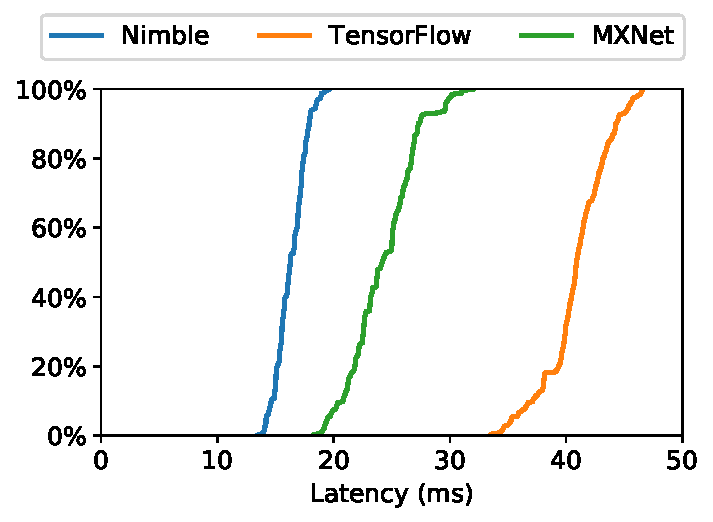
\includegraphics[height=5cm]{figs/bert_cdf_c5.pdf}
%     \caption{BERT latency CDF on Intel CPU.}
%     \label{fig:bert-cdf}
% \end{figure}

%\subsection{Optimization implications}
%\label{sec:eval:opt}
%\subsubsection{Memory planning}

%\subsubsection{Dynamic kernel dispatch}
\subsection{Microbenchmark}

% \begin{table}[t]
%     \centering
%     \begin{tabular}{c|cc|cc}
%         \toprule
%         \multirow{2}{*}{Device} & TVM & Relay  & kernel & others  \\
%         & lat. (ms) & lat. (ms) & lat. (ms) &  (ms) \\ %&  (\%) \\
%         \midrule
%         Intel  & 19.38 & 24.32 & 21.06 & 3.26 \\% & 13.4\%
%         ARM & 223.50 & 237.41 & 228.59 & 8.82 \\%& 3.72\% \\
%         Nvidia & 5.58 & 5.86 & 5.60 & 0.26 \\%& 4.44\% \\
%         \bottomrule
%     \end{tabular}
%     \caption{BERT model latency (sequence length 128) using TVM and Relay on different hardware.
%     {\it kernel latency} shows the latency of kernel invocation in Relay, and {\it others} shows the extra latency introduced by other instructions.
%     }
%     \label{tab:overhead}
%     \vspace{-1em}
% \end{table}

% \hide{
% \begin{figure}[t]
%     \centering
%     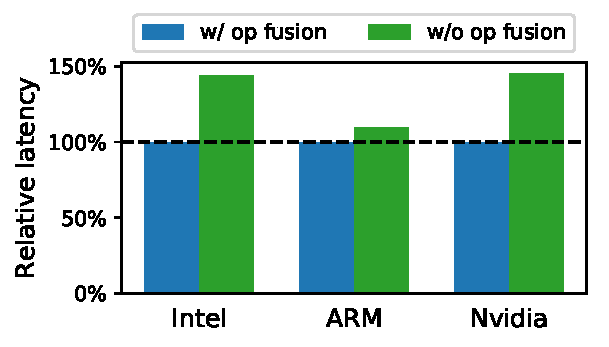
\includegraphics[height=3.5cm]{figs/op_fusion.pdf}
%     \caption{Relative latency comparison between Relay with and without operator fusion for BERT model with sequence length 128.}
%     \label{fig:fusion}
% \vspace{-1em}
% \end{figure}
% }

\begin{figure}[t]
    \centering
    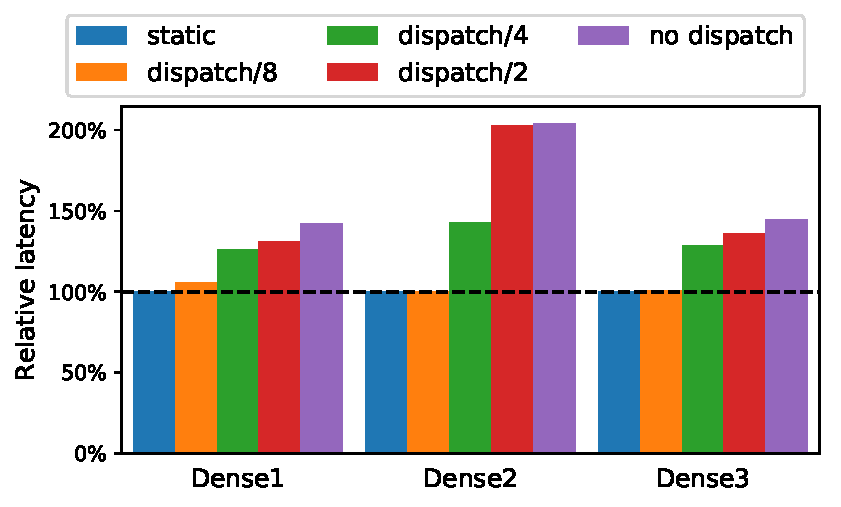
\includegraphics[height=4.5cm]{figs/sym_codegen.pdf}
    \caption{Relative latency comparison between symbolic codegen and static codegen of 3 dense operators on ARM CPU. The latency of kernel compiled with static shapes is used as the baseline. ``dispatch/$k$'' indicates that we generate $k$ symbolic kernels to be dispatched at runtime. ``no dispatch'' means that only one symbolic kernel is generated and therefore no dispatching is needed. %\protect\yida{The labels of x-axis, can we make them Dense 1, Dense 2 and Dense 3? L1, L2, L3 are like cache level to me at the first glance}
    }
    \label{fig:sym-codegen}
\end{figure}

This section analyzes the performance gain of Relay by using BERT as the microbenchmark. Three studies will be conducted to examine (a) the overhead introduced by the VM, %(b) the effectiveness of operator fusion\yida{Can we somehow relate this to any proposed techniques? For example, op fusion is enabled by carefully taking care of shape functions?},
(b) the advantage of the proposed memory planning pass, and (c) the performance discrepancy between symbolic and static codegen.

\noindent {\bf Overhead in handling dynamism} In order to understand the overhead that Relay spends to take care of dynamism, we compared it to TVM where static sequence length and TVM static runtime is used to execute BERT.
%\yida{how do you map this to the aforementioned four points?}
\autoref{tab:overhead} details the performance difference between Relay and TVM.  TVM is 5\% to 25\% faster than Relay on static shapes, though the absolute latency difference is small. The overhead comes from two aspects: (a) kernels generated with symbolic shapes cause extra overhead in the index computation. (b) other instructions in the virtual machine are required to handle the dynamic execution, such as shape functions, dynamic memory allocation, instruction dispatch, etc.
On Nvidia GPU, most of bytecode latency is overlapped with the GPU execution thanks to heterogeneous device placement (\autoref{sec:compliation:hetero}), and therefore the overhead of other instructions is negligible.

% \hide{
% \noindent {\bf Operator fusion}
% One of the most important benefits from deep learning compiler is its flexibility to fuse operators for better cache locality. \autoref{fig:fusion} depicts the comparison between Relay with and without operator fusion. With operator fusion, the latency can be reduced by 44\%, 10\%, and 46\% on Intel CPU, ARM CPU, and Nvidia GPU, respectively. This is because operator fusion provides better opportunities for (a) achieving better cache locality, and (b) reducing the buffer allocation for temporary intermediates as well as the number of shape functions to be executed.\yida{Mention that this is not available if we don't take care of the shape functions properly. Op fusion is not our contribution, but enabling it in the context of dynamism is.}}
%so that some memory copies and synchronization between devices as well as irregular memory accesses for calculating shapes can be possibly eliminated.

\noindent {\bf Memory planning} % Memory allocation at runtime is expensive.
\autoref{sec:compliation:memory} proposed memory planning to coalesce memory allocation together and reuse the already allocated memory chunks. Thanks to this pass, we are able to reduce the number of buffer allocation by 47\%, and the memory allocation latency is reduced by 75\% from 2.0 ms to 0.5 ms on Intel CPU. We also compared the memory usage of Relay with memory planning to TVM which statically analyze and pre-allocate memory on popular computer vision models such as ResNet~\citep{he2016deep}, MobileNet~\citep{howard2017mobilenets}, VGG~\citep{simonyan2014very} and SqueezeNet~\citep{iandola2016squeezenet}. It turned out that Relay leads up to 8\% more memory footprint.

\noindent {\bf Symbolic codegen} We selected 3 dense operators in the BERT model and compared the performance of symbolic codegen against static codegen on ARM CPU.
%\yida{Can we claim that similar observation can be got for other platforms? State it if yes (I know that the performance is worse than libraries, but we don't need to mention this)}.
\autoref{fig:sym-codegen} illustrates the relative latency of kernels generated with symbolic shapes to the baseline -- kernel compiled with static shapes. The auto-tuning algorithm chooses to tile the symbolic dimension corresponding to the dynamic sequence length by a factor of 8 in all three kernels. We varied the number of generated kernels to be dispatched during the symbolic codegen from 8 (full dispatch) to 1 (no dispatch) as described in \autoref{sec:compliation:codegen}. We observe that symbolic codegen with full dispatch can achieve nearly identical performance as that for static shapes. While reducing the number of kernels, latency increases up to 42\%, 104\%, and 45\% for these 3 layers, respectively.
We observe similar trends in dense operators with different shapes, other operators, and other platforms as well.



% \subsubsection{Memory pass}

% \subsubsection{Symbolic code generation}

% \subsubsection{VM overhead}
% \label{sec:eval:overhead}
% Finally, we compared the performance of model inference for static neural networks using Relay with unmodified TVM. TVM is known to be efficient in processing CNN models on various hardware platforms~\citep{tvm_osdi18, liu2019optimizing}. Relay extended TVM to support dynamism while inheriting the optimizations original TVM has. Relay's VM-based runtime was designed to be generic enough to handle static model inference as well. Therefore, comparing between Relay and the original TVM on static model inference should indicate how much overhead Relay introduces while introducing dynamic support.

% \autoref{fig:static-performance} and \autoref{fig:memory-overhead} show the latency and memory footprint comparison between Relay and original TVM on different static CNN models. The models were optimized via the TVM pipeline in both systems. The difference is that Relay uses its VM-based runtime while TVM uses its original graph runtime. From the figure we can tell that Relay's VM-based runtime adds minimal overhead compared to TVM's original runtime, by adding up to 13\% more execution time and 8\% more memory footprint. Also, \autoref{fig:memory-overhead} further testifies that our memory planning optimization reduces the memory usage on static model inference as well.

% We have evidence that this overhead is due to missing micro-optimizations, and not inherent to our approach, and should be erased over time.

% \begin{figure}
% \centering
% \input{figs/static_perf}
% \caption{Latency comparison between Relay and TVM on static model inference. The latency was tested for both systems on Intel CPUs, Nvidia GPUs and ARM CPUs by setting batch size=1. The latency of TVM on those platforms was normalized to 1, the lower the better.}
% \label{fig:static-performance}
% \end{figure}

% \begin{figure}
% \centering
% \input{figs/memory}
% \caption{Memory usage comparison between Relay and TVM on static models. Relay was done with and without optimization on memory planning. The results were obtained on Intel CPUs. Nvidia GPUs and ARM CPUs would lead to the identical results. The amount of memory used by TVM was normalized to 1, the lower the better.}
% \label{fig:memory-overhead}
% \end{figure}




\begin{comment}
\begin{figure*}[t]
  \centering
  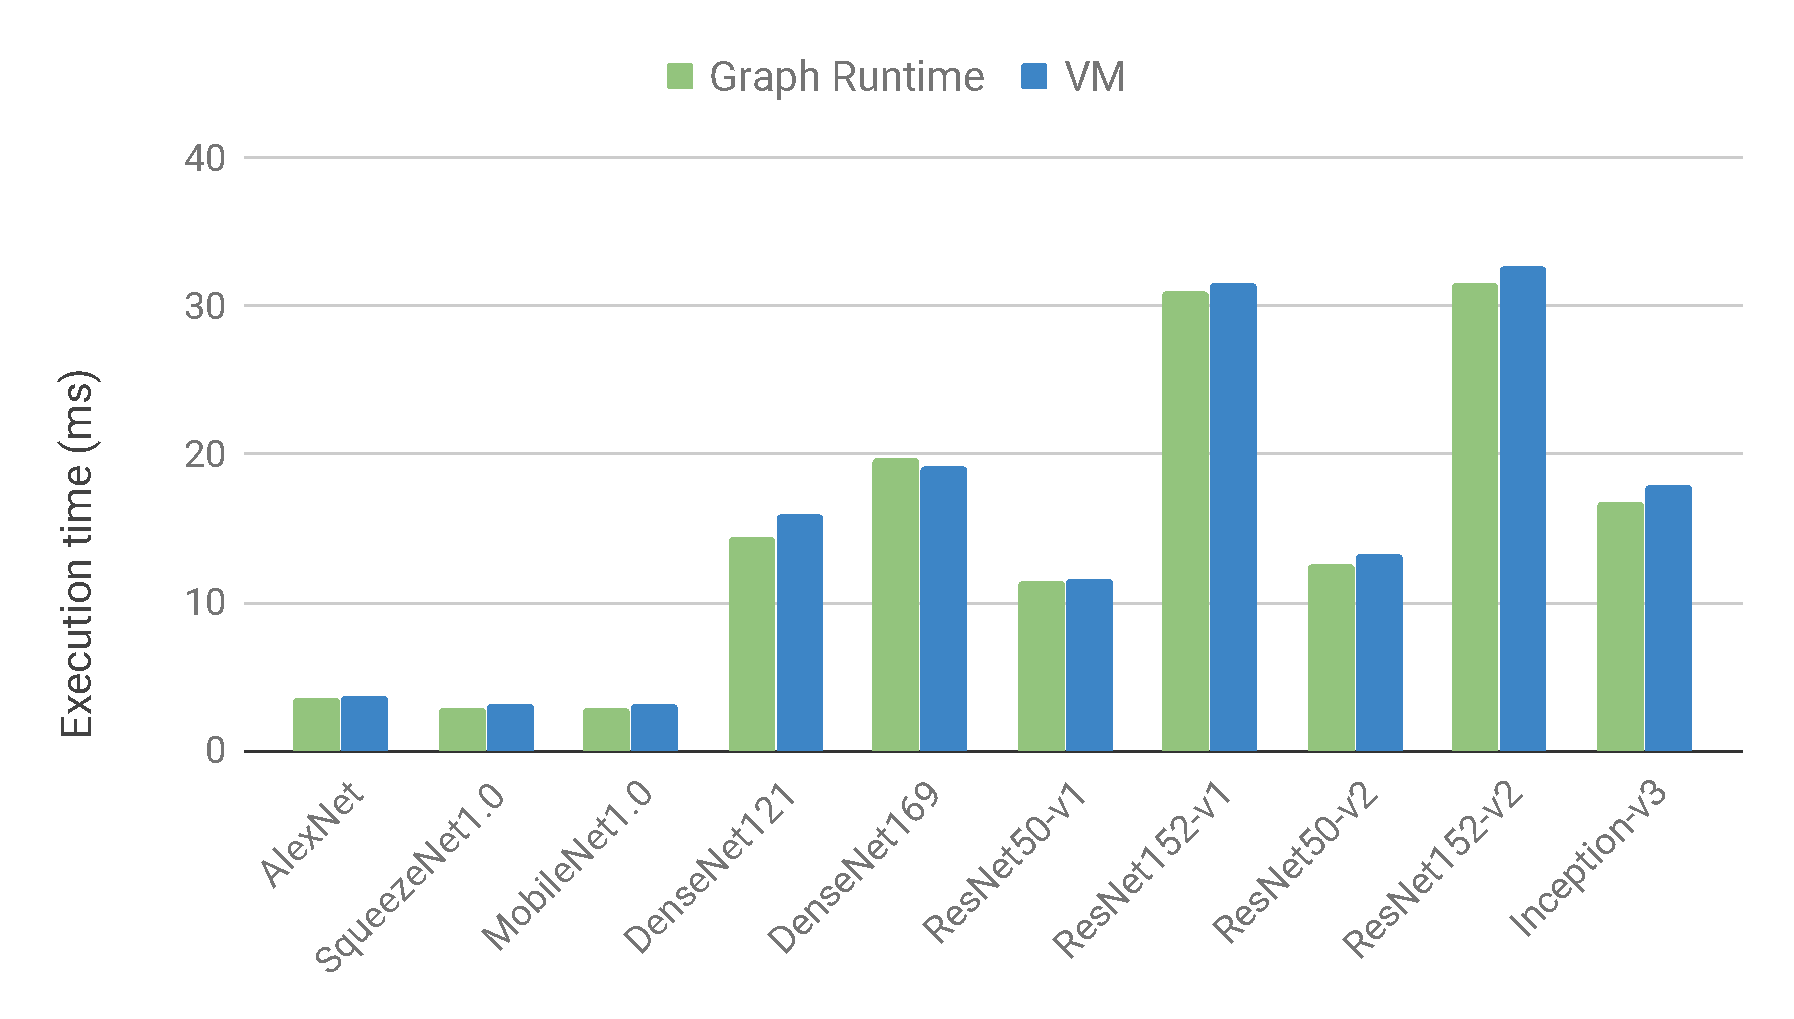
\includegraphics[width=.8\linewidth]{figs/cv_models.pdf}
  \caption{Benchmarking results of graph runtime vs. Relay.}
  \label{fig:benchmark}
\end{figure*}

\begin{table*}[t]
\centering
\begin{tabular}{llllrrc}
\toprule
\multicolumn{1}{c}{\multirow{2}{*}{input size}} & \multicolumn{1}{c}{\multirow{2}{*}{hidden size}} & \multicolumn{1}{c}{\multirow{2}{*}{\# layers}} & \multicolumn{1}{c}{\multirow{2}{*}{seq length}} & \multicolumn{2}{c}{latency (ms)}                         & \multicolumn{1}{c}{\multirow{2}{*}{speedup ($\times$)}} \\
\multicolumn{1}{c}{}                            & \multicolumn{1}{c}{}                             & \multicolumn{1}{c}{}                          & \multicolumn{1}{c}{}                            & \multicolumn{1}{c}{MxNet} & \multicolumn{1}{c}{Relay VM} & \multicolumn{1}{c}{}                             \\
\midrule
100                                             & 100                                              & 1                                             & 1                                               & 0.53                      & 0.03                         & 18.4                                             \\
100                                             & 100                                              & 1                                             & 20                                              & 4.74                      & 0.52                         & 9.2                                              \\
100                                             & 100                                              & 1                                             & 100                                             & 21.75                     & 2.57                        & 8.5                                              \\
100                                             & 100                                              & 2                                             & 100                                             & 30.53                     & 4.79                         & 6.4                                              \\
100                                             & 100                                              & 3                                             & 100                                             & 55.47                     & 7.04                         & 7.9                                              \\
200                                             & 600                                              & 3                                             & 100                                             & 67.14                     & 35.16                        & 1.9                                              \\
400                                             & 1150                                             & 3                                             & 100                                             & 166.54                    & 123.54                       & 1.3                                              \\
1500                                            & 1500                                             & 2                                             & 100                                             & 182.71                    & 138.78                       & 1.3
\\\bottomrule
\end{tabular}
\vspace{6pt}
\caption{Compare performance of LSTM models between MxNet and Relay VM.}
\label{tab:lstm}
\end{table*}

We evaluated the model inference with the VM against the TVM graph runtime on a number of popular vision models, including AlexNet, ResNet, MobileNet, VGG, DenseNet, SqueezeNet and Inception. Models are from GluonCV model zoo.  We repeated the inference 100 times for each model, obtained the performance result by averaging the execution times. All experiments were performed on Amazon EC2 C5.9xlarge instance (Intel Skylake-SP, 72 GiB memory, 18 physical cores, featured with AVX-512). In general, VM reached comparable inference performance even some optimizations were not plugged. As shown in \autoref{fig:benchmark}, we observed VM provided 2.59\% performance improvement on DenseNet169. On the rest of models, VM introduced some performance regression. We saw 11.3\% performance drop on SqueezeNet1.0.

We also evaluated the inference performance of recurrent models, which requires control flow support. We choose LSTM model \citep{hochreiter1997long} and vary the input size, hidden size, number of layers, and sequence length. We measured the execution time of LSTM models for both MxNet MKL 1.4.1 and Relay VM on Amazon EC2 C5.9xlarge instance. \autoref{tab:lstm} shows that Relay VM can achieve 6.4-18.4$\times$ speedup on small LSTM models and 1.3-1.9$\times$ speedup on larger models.
\end{comment}

% \chapter{Program optimization for non-experts: Dataflow Rewriting}
\label{ch:opt_for_non_experts}

% Execution
% VM Compiler/Aot
\chapter{Compiling Relay}
\label{ch:compiler}


\subsection{Compiler Framework}

The process for compiling Relay proceeds in three stages.
First, the frontend converts input formats into the Relay IR.
Next, the Relay compiler typechecks and optimizes the program
  to produce the final program.
After performing optimizations,
  the Relay backend transforms
  the Relay program into a form that can be executed on
  the intended hardware, based on the specified execution mechanism.
The backend additionally lowers Relay operators into a TVM expression,
  computes a schedule for the final TVM expression, and lowers it into
  native code.

\subsection*{Frontend}

There are several ways to write an Relay program.
A user can build an in-memory representation of
  a program in C++ or Python,
  parse one written in the Relay text format,
  load one from the on-disk serialization format,
  or import one from popular frameworks and interchange formats
    (e.g., TensorFlow, MxNet, Keras, DarkNet, and ONNX).
Many frameworks and interchange formats use static computation graph-based representations,
  which can easily be translated into Relay.
A greater challenge is translating frameworks
  with a richer computation model such as TensorFlow (TF).
TF supports control flow and includes \verb|TensorArray|, a write-once
  tensor container.
We can extract the loop structure out of the TF graph, converting
  it to an Relay loop, and transform the \verb|TensorArray| into an Relay list.
Once new deep learning languages and IRs under development
  are stable it is likely they can be translated into Relay (see
  Section~\ref{sec:pl_techniques_in_dl}).
PyTorch provides an expressive programming model, and is a good fit
  for Relay, which has integration into PyTorch's JIT infrastructure,
  enabling users to transparently use Relay for improved performance.

\subsection*{Compiler}
Once an Relay abstract syntax tree (AST) is produced,
  the program is optimized by applying a series of Relay-to-Relay
  passes.
Between each pass, Relay performs type inference and checking,
  rejecting malformed programs as well as populating shape and type
  information that passes can utilize.
The Relay compiler supports traditional optimizations
  (e.g., constant folding, common subexpression elimination, and dead code elimination)
  and domain-specific optimizations
  (see Sec.~\ref{sec:optimizations}).

\subsection*{Backends}

Relay produces machine-specific code
  by decomposing the problem of code generation into multiple distinct phases.
Relay translates all operators into \tvm expressions
  to produce dense linear algebra kernels~\citep{tvm_osdi18, tensor_comprehensions, halide}.
\tvm produces low-level operators that expect a fixed calling convention,
  as well as preallocated inputs and outputs.
The result is an object file containing hardware-specific implementations of all
  operations.
The remaining Relay program then is executed or compiled,
  with operator invocations replaced by calls to the optimized operators.
By representing operators as \tvm expressions, we can programmatically
  transform them and automatically generate new implementations for the transformed operators.
Optimizations like fusion and quantization
  rely on this novel behavior.
After primitive operators are lowered,
  the remaining Relay program ties
  together operator invocations, allocation, control-flow,
  recursion, and high-level data structures.
There are multiple options for executing the combined full program:
  the Relay interpreter (with JIT compilation),
  an Relay virtual machine,
  the \tvm graph runtime,
  and an experimental Relay ahead-of-time compiler
  that converts programs to C++ to produce a target-specific binary.
% We are able to target CPU, GPU,
%   iOS and Android mobile devices,
%   custom accelerators, and FPGAs.

% % EVAL

% We evaluate Relay on several systems and over a diverse set of vision and NLP workloads to
%   demonstrate that (1) Relay enables \emph{expressive} programs via a large breadth
%   of models, (2) Relay supports \emph{composition} of program-level optimizations
%   such as quantization and fusion, and (3) Relay provides
%   \emph{portability} by targeting a number of hardware backends.
% Not only does Relay provide these three properties, we do so while also demonstrating
%   competitive performance.
% Relay is an open-source academic project.\footnote{Relay is publicly available at [redacted for review].}
%   It has been deployed at a popular web service provider,
%     a telecommunications and consumer electronics manufacturer,
%     and a social media company, among others.
%     Our evaluation demonstrates Relay's competitive performance for a
%     broad class of models and devices
%     (CPUs, GPUs, and emerging accelerators).
%   Relay's design demonstrates how a unified IR can provide
%     expressivity, composability, and portability
%     without compromising performance.


%   We evaluate Relay on several systems and over a diverse set of vision and NLP workloads to
%   demonstrate that (1) Relay enables \emph{expressive} programs via a large breadth
%   of models, (2) Relay supports \emph{composition} of program-level optimizations
%   such as quantization and fusion, and (3) Relay provides
%   \emph{portability} by targeting a number of hardware backends.
% Not only does Relay provide these three properties, we do so while also demonstrating
%   competitive performance.
% Relay is an open-source academic project.\footnote{Relay is publicly available at [redacted for review].}
%   It has been deployed at a popular web service provider,
%     a telecommunications and consumer electronics manufacturer,
%     and a social media company, among others.

\subsection{Compiler Framework}

The process for compiling Relay proceeds in three stages.
First, the frontend converts input formats into the Relay IR.
Next, the Relay compiler typechecks and optimizes the program
  to produce the final program.
After performing optimizations,
  the Relay backend transforms
  the Relay program into a form that can be executed on
  the intended hardware, based on the specified execution mechanism.
The backend additionally lowers Relay operators into a TVM expression,
  computes a schedule for the final TVM expression, and lowers it into
  native code.



  \subsection*{Frontend}

  There are several ways to write an Relay program.
  A user can build an in-memory representation of
    a program in C++ or Python,
    parse one written in the Relay text format,
    load one from the on-disk serialization format,
    or import one from popular frameworks and interchange formats
      (e.g., TensorFlow, MxNet, Keras, DarkNet, and ONNX).
  Many frameworks and interchange formats use static computation graph-based representations,
    which can easily be translated into Relay.
  A greater challenge is translating frameworks
    with a richer computation model such as TensorFlow (TF).
  TF supports control flow and includes \verb|TensorArray|, a write-once
    tensor container.
  We can extract the loop structure out of the TF graph, converting
    it to an Relay loop, and transform the \verb|TensorArray| into an Relay list.
  Once new deep learning languages and IRs under development
    are stable it is likely they can be translated into Relay (see
    Section~\ref{sec:pl_techniques_in_dl}).
  PyTorch provides an expressive programming model, and is a good fit
    for Relay, which has integration into PyTorch's JIT infrastructure,
    enabling users to transparently use Relay for improved performance.

  \subsection*{Compiler}
  Once an Relay abstract syntax tree (AST) is produced,
    the program is optimized by applying a series of Relay-to-Relay
    passes.
  Between each pass, Relay performs type inference and checking,
    rejecting malformed programs as well as populating shape and type
    information that passes can utilize.
  The Relay compiler supports traditional optimizations
    (e.g., constant folding, common subexpression elimination, and dead code elimination)
    and domain-specific optimizations
    (see Sec.~\ref{sec:optimizations}).

  \subsection*{Backends}


  Relay produces machine-specific code
    by decomposing the problem of code generation into multiple distinct phases.
  Relay translates all operators into \tvm expressions
    to produce dense linear algebra kernels~\citep{tvm_osdi18, tensor_comprehensions, halide}.
  \tvm produces low-level operators that expect a fixed calling convention,
    as well as preallocated inputs and outputs.
  The result is an object file containing hardware-specific implementations of all
    operations.
  The remaining Relay program then is executed or compiled,
    with operator invocations replaced by calls to the optimized operators.
  By representing operators as \tvm expressions, we can programmatically
    transform them and automatically generate new implementations for the transformed operators.
  Optimizations like fusion and quantization
    rely on this novel behavior.
  After primitive operators are lowered,
    the remaining Relay program ties
    together operator invocations, allocation, control-flow,
    recursion, and high-level data structures.
  There are multiple options for executing the combined full program:
    the Relay interpreter (with JIT compilation),
    an Relay virtual machine,
    the \tvm graph runtime,
    and an experimental Relay ahead-of-time compiler
    that converts programs to C++ to produce a target-specific binary.


  \subsection{Backends}
  After primitive operators are lowered,
    the remaining Relay program is the glue that ties
    together operator invocations, allocation, control-flow,
    recursion, and high-level data structures.
  There are multiple options for executing the combined full program:
      the Relay interpreter (with JIT compilation),
      the \tvm graph runtime,
      and an ahead-of-time compiler
      that converts programs to C++.
  % We are able to target CPU, GPU,
  %   iOS and Android mobile devices,
  %   custom accelerators, and FPGAs.

  \subsection{Compiler Framework}
  The Relay pipeline can be split into three classic components:
    the frontend, where input formats are translated to Relay;
    the compiler, which type checks Relay ASTs, applies optimizations,
      and compiles operators;
    and the backend, where an execution mechanism is selected and
      available hardware accelerators are utilized.

  \subsection{Frontend}

  There are several ways to write an Relay program.
  A user can build an in-memory representation of
    a program in C++ or Python;
    parse one written in the Relay text format;
    or load one from the on-disk serialization format,
    similar in design to LLVM's bitcode.
  Models from popular frameworks, including
    TensorFlow, PyTorch, MxNet, Keras, and DarkNet, as well as interchange
    formats, such as ONNX, may be imported directly into Relay.
  \subsection{Compiler}
  Once an Relay abstract syntax tree (AST) is produced,
    the program is optimized by applying a series of Relay-to-Relay
    passes.
  Between each pass, Relay performs type inference and checking,
    rejecting malformed programs as well as populating shape and type
    information that passes can utilize.
  Relay optimizations consist of both traditional compiler
    optimizations as well as domain-specific optimizations.
  Traditional compiler optimizations include constant folding,
    common subexpression elimination,
    and dead code elimination.
  DL-specific optimizations include
    operator fusion,
    quantization,
    layout transformation,
    and accelerator-specific optimizations.

  Relay produces machine-specific code
    by decomposing the problem of code generation into multiple distinct phases.
  % See Figure~\ref{fig:pipeline} for a visual overview of each stage.
  Since Relay is a high-level IR, it depends on a low-level code generator,
    such as \tvm or Halide,
    to produce dense linear algebra kernels~\citep{tvm_osdi18, halide}.
  We use \tvm in our experiments.
  Low-level kernel compilers focus on generating highly efficient operators.
  The generated kernels have a fixed calling convention and do not
    handle allocation. Instead, they expect inputs and outputs to be preallocated.
  From an optimized AST,
    the compiler extracts a set of Relay operators,
    translates them to TVM expressions,
    and then compiles to available hardware targets.
  The resulting output is an
    object file that contains the compiled operators
    and an Relay program that invokes these primitives.
  In our prototype implementation,
    we are able to target CPU, GPU,
    iOS and Android mobile devices,
    custom accelerators, and FPGAs.

% \chapter{Supporting Hardware Accelerators}
\label{ch:accel}

BYOC

\subsection{VTA}

Hardware specialization is a powerful way to accelerate
  a known set of applications and workloads.
A component of \relay is lowering high-level programs down
  to the bespoke semantics of emerging hardware accelerators.
Unfortunately, deep learning (DL) is anything but a static field, and the machine learning (ML) community
  rapidly changes how they use to write models, the architecture of models themselves, the operators
  used by said models, and the data types they operate over.
Initial programmable accelerators~\citep{tpuv1} offer potentially huge performance
  improvements at the cost of complex specialized compilation.
Furthermore the churn of machine learning has lead to an interest
  in customizable designs, with features such as new numeric representations,
  new hardware engines, and more.
In order to customize the behavior of accelerators designs, even when open-sourced,
  there is a need for the availability of a transparent and modular software stack.
An end-to-end approach requires integration of frameworks, systems, compilers,
  and architecture in order to execute state-of-the-art ML using hardware acceleration.
Peak FLOPs provide value only if a programmer can access them.
In order to tackle this problem I have collaborated on the design for \vta (Versatile Tensor Accelerator),
  an explicitly programmed accelerator paired with a compiler and runtime that can evolve
  in tandem with deep learning models without sacrificing the advantages of specialization.

\vta makes following contributions:

\begin{itemize}
    \item \emph{A programmable accelerator design} that exposes a two-level programming interface: a high-level task ISA to allow explicit task scheduling by the compiler stack, and a low-level microcode ISA to provide software-defined operational flexibility.
    In addition, the \vta architecture is fully parameterizable: the hardware intrinsics, memories, and data types can be customized to adapt the hardware backend requirements.
    \item \emph{An extensible runtime system} for heterogeneous execution that performs JIT compilation of microcoded kernels to provide operational flexibility. For example, the \vta runtime lets us extend the functionality of \vta's original computer-vision-centric design to support operators found in style transfer applications without requiring any hardware modifications.
    \item \emph{A schedule auto-tuning platform} that optimizes data access and reuse in order to rapidly adapt to changes to the underlying hardware and to workload diversity.
\end{itemize}

We recently published a paper on VTA in IEEE Micro Journal Special Issue
  on Deep Learning Acceleration.
\vta is a powerful part of doing research, and \relay is a critical part of the research agenda
  being pursued in the SAMPL lab, with recent funding to explore directly mapping \relay programs
  on to \vta as well as a diverse set of accelerators, and is related to the final topic of my
  thesis automatic tensorization.

% Future Work/Conclusion
\chapter{Future Work}
\label{ch:future}

This thesis demonstrates a principled approach to optimizing dynamic neural networks
    that generalizes the performance enjoyed by static neural networks to a greater
    number of networks.
There are still open questions on how to optimize and compile
    generic tensor programs to arbitrary hardware targets.
TVM is continuing to evolve rapidly
    with many changes in the past year not detailed
    in this thesis.
In particular completing the IR unification, improved
    dynamic model support, training support, automatic
    scheduling for new hardware targets and much more.
The remainder of this section touches on some of the
    challenges that lie in front of this work.

\subsection{Unified IR}

TVM has been working on unifying its multiple levels of
    IR into a family of dialects which can invoke functions
    at different level of abstractions.
The start of this work is complete but using the
    new unified world to meaningfully improve optimizations
    is something that has not yet been demonstrated.
For example one could lower an entire Relay program
    to a single GPU kernel using the new machinery,
    but no one has attempted such an optimization yet.

\subsection{Going further with Dynamic Models}

There are still problems which are unsolved in Relay's
    current iteration.
There are analyses that can be further improved such as
    recover further static shape information for optimization
    using a more precise analysis.
Or features not yet supported such as dynamically ranked tensors.
There are still interesting challenges to solve here as
    models evolve and demand more from compilers.s

\subsection{Training Support}

A team at OctoML and AMD have begun work on using TVM
    to accelerate training by building a framework
    that lowers all computation to Relay which
    can make use of all the techniques described
    in this thesis.
Although the work just began we were able to
    get models working on AMD GPUS with no custom
    code needed a feat most frameworks have
    failed to achieve.
There significant work to make this a state
    of the art competitive approach with existing
    frameworks but an interesting area going forward
    as TVM allows training to be deployed to any
    supported device.

\subsection{Automatic Scheduling}

A final promising area being explored at OctoML is
    automatic scheduling of tensor programs, including
    tensorization.
Originally in TVM a user must provide the network,
    operator definitions, and schedules.
AutoTVM introduced the ability to define a template
    schedule where some parameters such as tiling
    factor, or loop split can be learned using ML.
Ansor then introduced ability to learn both the
    template and the parameters using ML guided
    search.
The finally vision of these systems is to allow
    a Relay program to be lowered to TVM's TIR
    and then scheduled automatically allowing
    users to interpolate between manually
    knowledge and fully automatically.
This would enable users to leverage the
    expressivity of Relay, then lower to TIR,
    and finally rewrite the code to achieve
    near optimal performance using ML guided
    search.

These directions represent potentially years more work, and will be hopefully
    realized by collaborators PhD theses, future publications, the open source
    community and development teams at OctoML.
The work done in this this presents a compelling foundation on which to build
    these future efforts.


%----------------------------------------------------------------------------------------

\backmatter


\section{Appendix}

\begin{figure}
  \begin{center}
    \begin{minipage}{0.5\textwidth}
      \begin{minted}{ocaml}
                    const(v, sh, dt)
      \end{minted}
    \end{minipage}
  \end{center}
  $\Downarrow$
  \begin{center}
    \begin{minipage}{0.5\textwidth}
      \begin{minted}{ocaml}
        (const(v, sh, dt), ref(const(0, sh, dt)))
      \end{minted}
    \end{minipage}
  \end{center}
  \vspace{0.25cm}
  \begin{center}
    \begin{minipage}{0.5\textwidth}
      \begin{minted}{ocaml}
    op : fn<>(a_1 : T1, ..., a_n : Tn) -> O
      \end{minted}
    \end{minipage}
  \end{center}
  $\Downarrow$
  \begin{center}
    \begin{minipage}{0.5\textwidth}
      \begin{minted}[mathescape=true]{ocaml}
def @op_grad<>(a_1 : type_transform(T1), ...,
    a_n : type_transform(Tn))
    -> type_transform(O) {
  let %r = rev_op<>(a_1, ..., a_n);
  let %ref = ref(zeros_like<>(r.0));
  let %bpv = !bp;
  let %nbp = def @bpf<>() -> () {
    let %grad = (r.1)(!ref);
    a_1.1 := add<>(!(a_1.1), grad.0);
    ...
    a_n.1 := add<>(!(a_n.1), grad.(n-1));
    bpv()
  }
  bp := nbp;
  (r.0, ref)
}
      \end{minted}
    \end{minipage}
  \end{center}
  \caption{
    The above depicts the AD expression
      transformation macro.
    The macro takes as an
      argument an expression AST and a backpropagator
      \texttt{bp}
      (a reference to a function that takes no
      arguments and returns unit,
      which serves to update the reverse value references)
      and recurses down the expression's AST,
      making the above substitutions wherever
      it encounters a tensor constant or an operator
      \texttt{op}.
    All other AST constructs are unchanged by the macro.
    For simplicity, type arguments and relations
      are omitted in this figure;
      at present, \relay does not
      support type arguments in gradients.
    Note that the macro \texttt{type\_transform}$(T)$
      similarly recurses down the AST of the type $T$
      and replaces all tensor types with a
      pair of a tensor type
      and a reference to a tensor type
      (the first member is the forward value;
      the second, a reference to the reverse value)
    For a given operator \texttt{op},
      \texttt{rev\_op} refers to the registered reverse function.
    Additionally, for brevity,
      a semicolon without a \texttt{let}
      is used above as a sequence operator,
      namely a let node in which the bound
      variable is disregarded.}
  \label{fig:ad-expr-transform}
\end{figure}

\begin{figure}
  \begin{minted}{ocaml}
def @grad_f<>(a_1 : T1, ..., a_n : Tn)
    -> (O, (T1, ..., Tn)) {
  let %bp = ref(def @bpf<>() -> () { () });
  let %p_1 = (a_1, ref(zeros_like<>(a_1)));
  ...
  let %p_n = (a_n, ref(zeros_like<>(a_n)));
  let %c = (autodiff(bp, f))<>(p_1, ..., p_n);
  c.1 := ones_like<>(c.0);
  (!bp)();
  (c.0, (!(p_1.1), ..., !(p_n.1)))
}
  \end{minted}
  \caption{The gradient \relay{}'s AD produces
    for a function \texttt{f} of type
    \texttt{fn}$\langle\rangle(T_1, \ldots T_n) \rightarrow O$.
  The gradient function returns a tuple of
    the forward value of the function
    (simply evaluating the function at the arguments)
    and a tuple containing the
    partial derivative with respect to each argument.
  \texttt{autodiff} refers to the macro described in
    Fig. \ref{fig:ad-expr-transform}.
  As with Fig. \ref{fig:ad-expr-transform},
    the present implementation of
    \relay{}'s AD does not handle type relations or type arguments,
    so they are omitted in this figure.
  Also as in Fig. \ref{fig:ad-expr-transform},
    semicolons wihout \texttt{let} bindings
    are used as sequence operators for convenience.}
  \label{fig:ad-gradient}
\end{figure}

% \begin{figure}[H]
  \begin{jmpgrammar}
    \bnfrule{REAL}{\real} \is{\mathbb{R}}\\
    \bnfrule{NAT}{\nat} \is{\mathbb{N}}\\
    \bnfrule{NAME}{\rName} \is{\texttt{(}\text{`\_'}\inlineAlt[a-zA-Z]\texttt{)}\ \
    \atLeastZero{\text{`\_'}\inlineAlt[a-zA-Z]\inlineAlt[0-9]}}\\
    \bnfrule{TYPE NAME}{\typename} \is{[A-Z]\ \ \atLeastZero{\text{`\_'}\inlineAlt[a-zA-Z]\inlineAlt[0-9]}}\\
    \bnfrule{GLOBAL VAR}{\gvar} \is{\kwd{@}\rName}\\
    \bnfrule{LOCAL VAR}{\lvar} \is{\kwd{\%} \rName}\\
    \bnfrule{GRAPH VAR}{\graphVar} \is{\kwd{\%} \nat}\\
    \bnfrule{TYPE VAR}{\tyvar} \is{\rName}\\
    \bnfrule{OPERATOR}{\op} \is{\rName}\\\\
    \bnfrule{Program}{\program} \is{\atLeastOne{\defn\inlineAlt\typedef}}
      \alt{\expr}\\\\
    \bnfrule{Param}{\param} \is{\rParamRule}\\
    \bnfrule{Type Param}{\tyParam} \is{\rTyParamRule}\\\\
    \bnfrule{Definition}{\defn} \is{\rDefnRule}\\\\
    \bnfrule{Type Definition}{\typedef} \is{\rTypeDefRule}\\\\
    \bnfrule{Kind}{\kind} \is{\kwd{BaseType}}
      \alt{\kwd{Shape}}
      \alt{\kwd{Relation}}
      \alt{\kwd{ADT}}
      \alt{\kwd{Type}}\\\\
    \bnfrule{BaseType}{\basetype} \is{\kwd{int} \nat \maybe{\kwd{x} \nat}}
      \alt{\kwd{float} \nat \maybe{\kwd{x} \nat}}
      \alt{\kwd{bool} \maybe{\nat}}\\\\
    \bnfrule{Shape}{\shape} \is{\kwd{(} \seq{\nat} \kwd{)}}\\\\
    \bnfrule{Pattern}{\patt} \is[constructor]{\op \kwd{(} \seq{\patt} \kwd{)}}
      \alt[wildcard]{\wildcard}
      \alt[variable]{\lvar\ \maybe{\typeanno}}
  \end{jmpgrammar}
\end{figure}
\begin{figure}[H]
  \ContinuedFloat
  \begin{jmpgrammar}
    \bnfrule{Expr}{\expr} \is[local var]{\lvar}
      \alt[global variable]{\gvar}
      \alt[constant tensor]{\kwd{const} \kwd{(} \texttt{(}\real\inlineAlt\bool\texttt{)} \kwd{,} \shape \kwd{,} \basetype \kwd{)}}
      \alt[call]{\expr \maybe{\tyargs} \args\vspace{0.2em}}
      \alt[let]{\rLetRule}
      \alt[\kwd{let}\ \kwd{\%}\_\ \kwd{=}\ \expr\kwd{;}\ \expr]{\rAnonLetRule}
      \alt[graph let]{\rGraphLetRule}
      \altSpace{0.5em}{function}{\rFnRule}
      % \altSpace{1em}{type cast?}{\kwd{(} \type \kwd{)} \expr}
      \altSpace{1em}{tuple}{\rTupRule}
      \alt[tuple proj.]{\rTupProjRule}
      \alt[if-else]{\rIfElse{\expr}{\expr}{\expr}}
      \altSpace{0.5em}{pattern match}{\rMatchRule}
      \altSpace{1em}{operator}{\op}
      % TODO: Add this case back when we readd grad as a first-class construct.
      % \alt[gradient]{\kwd{grad}\kwd{(}\expr\kwd{)}}
      \alt[new ref]{\kwd{ref}\kwd{(}\expr\kwd{)}}
      \alt[get ref]{\kwd{!} \expr}
      \alt[set ref]{\expr \kwd{:=} \expr}\\\\
    \bnfrule{Type}{\type} \is[base type]{\basetype}
      \alt[shape]{\shape}
      \alt[tensor type]{\kwd{Tensor} \kwd{[} \shape \kwd{,} \basetype \kwd{]}}
      \alt[type variable]{\tyvar}
      \alt[function type]{
        % \begin{split}
        \kwd{fn}\ &\rTyParamsRule \kwd{(} \seq{\type} \kwd{)}\ \rettype\\
        &\maybe{\relations}
        % \end{split}
        }
      \alt[ref type]{\kwd{Ref} \kwd{[} \type \kwd{]}}
      \alt[tuple type]{\kwd{(} \seq{\type} \kwd{)}}
      \alt[type call]{\type \kwd{[} \seq{\type} \kwd{]}}
      \alt[type name]{\typename}
  \end{jmpgrammar}
  % \caption{The full BNF Grammar for the Relay{} language.}
  % \label{ref:lang_def}
\end{figure}

% \begin{figure}[H]
   \judgbox{\rstep{\rstate{\rnamespace}{\rheap}{\expr}}{\rstate{\rnamespace'}{\rheap'}{\expr'}}}{}
\begin{inference}
   \jmpInfer{Semantics-Closure}
      {}
      {{\begin{array}{l}
      \Gamma; \Delta \colon \texttt{def @} f \kwd{<} T_{m+1}, \ldots, T_n \kwd{>} (a_1 : T_1, \ldots a_m : T_m) \, \kwd{->} \, O \\
      \kwd{ where } R_1, \ldots, R_r, body \Rightarrow \\
      \Gamma; \Delta \colon \kwd{Closure}(f, body, \\
      \{ v \mapsto V \, | \, v \in \kwd{FreeVars}(body) \land v \mapsto V \in \Gamma \})
      \end{array}{l}}}
\jmpInfer{Semantics-Id}
      {id \mapsto V \in \Gamma}
      {\rstep{\rstate{\rnamespace}{\rheap}{id}}{\rstate{\rnamespace}{\rheap}{V}}}
\jmpInfer{Semantics-Product}
      {\forall i \in [1, n],
      \rstep{\rstate{\rnamespace}{\rheap_{i-1}}{E_i}}{\rstate{\rnamespace}{\rheap_i}{V_i}}}
      {\rstep{\rstate{\rnamespace}{\rheap_0}{\kwd{(} E_1 \kwd{,} \ldots \kwd{,} E_n \kwd{)}}}{\rstate{\rnamespace}{\rheap_n}{(V_1, \ldots, V_n)}}}
\jmpInfer{Semantics-Projection}
      {\Gamma; \Delta \colon E \Rightarrow \Gamma; \Delta^\prime \colon \kwd{(}V_1 \kwd{,} \ldots \kwd{,} V_n \kwd{)} \andalso i \in [0, n)}
      {\Gamma; \Delta \colon E \kwd{.} i, s \Rightarrow \Gamma; \Delta^\prime \colon V_{i + 1}}
\jmpInfer{Semantics-If-True}
      {\rstep{\rstate{\rnamespace}{\rheap}{C}}{\rstate{\rnamespace}{\rheap^\prime}{\rTrue}}\\
      \rstep{\rstate{\rnamespace}{\rheap^\prime}{B_1}}{\rstate{\rnamespace}{\rheap^{\prime\prime}}{V}}}
      {\rstep{\rstate{\rnamespace}{\rheap}{\rIfElse{C}{B_1}{B_2}}}{\rstate{\rnamespace}{\rheap^{\prime\prime}}{V}}}
\jmpInfer{Semantics-If-False}
      {\rstep{\rstate{\rnamespace}{\rheap}{C}}{\rstate{\rnamespace}{\rheap^\prime}{\rFalse}}\\
      \rstep{\rstate{\rnamespace}{\rheap^\prime}{B_2}}{\rstate{\rnamespace}{\rheap^{\prime\prime}}{V}}}
      {\rstep{\rstate{\rnamespace}{\rheap}{\rIfElse{C}{B_1}{B_2}}}{\rstate{\rnamespace}{\rheap^{\prime\prime}}{V}}}
\jmpInfer{Semantics-Ref-Create}
      {\Gamma; \Delta \colon C \Rightarrow \Gamma; \Delta^\prime \colon V}
      {\Gamma; \Delta \colon \kwd{Ref}\ C \Rightarrow \Gamma; \Delta^\prime
      \cup \{ v \mapsto V \} \colon \kwd{Ref}(v) \andalso \kwd{fresh}(v)}
\jmpInfer{Semantics-Ref-Read}
      {\Gamma; \Delta \colon C \Rightarrow \Gamma; \Delta^\prime \colon \kwd{Ref}(v) \andalso v \mapsto V \in \Delta^\prime}
      {\Gamma; \Delta \colon \kwd{!} C \Rightarrow \Gamma; \Delta^\prime \colon V}
\jmpInfer{Semantics-Ref-Write}
      {\\ \Gamma; \Delta \colon C \Rightarrow \Gamma; \Delta^\prime \colon \kwd{Ref}(v)
      \\ \Gamma; \Delta^\prime \colon N \Rightarrow \Gamma; \Delta^{\prime\prime} \colon V}
      {\Gamma; \Delta \colon C := N \Rightarrow \Gamma; \Delta^{\prime\prime}
      \cup \{ v \mapsto V \} \colon ()}
\end{inference}
\end{figure}

\begin{figure}[H]
   \ContinuedFloat
   \begin{inference}
\jmpInfer{Semantics-Let}
      {\Gamma; \Delta \colon C \Rightarrow \Gamma; \Delta^\prime \colon V
      \\ \Gamma \cup \{ id \mapsto V \}; \Delta^\prime \colon E \Rightarrow \Gamma \cup \{ id \mapsto V \}; \Delta^{\prime\prime} \colon V^\prime}
      {\Gamma; \Delta \colon \kwd{let \%} id\ \kwd{=}\ C \kwd{;}\ E \Rightarrow \Gamma; \Delta^{\prime\prime} \colon V^\prime}
\jmpInfer{Semantics-Call}
      {{\begin{array}{l}
      \Gamma; \Delta \colon C \Rightarrow \Gamma; \Delta_0^\prime \colon
      \kwd{Closure}(f, body, vars) \\
      \forall i \in [1, m], \Gamma; \Delta_{i - 1}^\prime \colon A_i
      \Rightarrow \Gamma; \Delta_i^\prime \colon V_i \\
      \end{array}}}
      {{\begin{array}{l}
      \Gamma; \Delta \colon C \kwd{<}T_{m + 1}, \ldots, T_n \kwd{>}(A_1,
      \ldots, A_m) \Rightarrow \Gamma; \Delta_m^{\prime\prime} \colon
      V^\prime \\
      \hspace{-0.5em} \Gamma \cup vars \cup \{ a_i \mapsto V_i \, | \, i \in [1, m] \} \, \cup \\
         \hspace{0.5em} \{ f \mapsto \kwd{Closure}(f, body, vars) \}; \Delta_m^\prime \colon body \Rightarrow \Gamma; \Delta_m^{\prime\prime} \colon V^\prime
      \end{array}{l}}}
\jmpInfer{Semantics-ADT-Constructor}
      {\\ \forall i \in [1, n], \Gamma; \Delta_{i - 1} \colon A_i \Rightarrow \Gamma; \Delta_i \colon V_i}
      {\Gamma; \Delta_0 \colon ADT_{C_j}(A_1, \ldots, A_n) \Rightarrow \Gamma; \Delta_n \colon ADT_{C_j}(V_1, \ldots, V_n)}
\jmpInfer{Semantics-ADT-Match}
      {\\ \Gamma; \Delta \colon s \Rightarrow \Gamma; \Delta^\prime \colon ADT_{C_i}(V_1, \ldots, V_n)
      \\ \Gamma \cup \{ a_i \mapsto V_i \, | \, i \in [1, n] \}; \Delta^\prime \colon E \Rightarrow \Gamma; \Delta^{\prime\prime} \colon V^\prime}
      {\Gamma; \Delta \colon
      {\begin{array}{l}
         \hspace{-0.5em} \kwd{match(}s\kwd{) \{}\\
         \hspace{0.5em} \kwd{|} \, C_1\kwd{(}a_1\kwd{,} \ldots\kwd{,} a_n\kwd{) => } e_1 \\
         \hspace{0.5em} \kwd{|} \, \ldots \, \kwd{|} \, C_i\kwd{(}a_1\kwd{,} \ldots\kwd{,} a_n\kwd{) => } E \\
         \hspace{0.5em} \kwd{|} \, \ldots \, \kwd{|} \, C_m\kwd{(}a_1\kwd{,} \ldots\kwd{,} a_n\kwd{) => } e_m \\
         \hspace{-0.5em} \kwd{\}}
      \end{array}}
      \Rightarrow \Gamma; \Delta^{\prime\prime} \colon V^\prime}
   \end{inference}
  \caption{A simplified operational semantics of \relay{}. All tensors are values, so boolean,
    integer, and floating point literals are irreducible per the above rules, as are tensors of other shapes. Thus, the values in \relay{} are tensors,
    closures, operators (functions whose bodies are opaque to \relay{}), products of values, references of values,
    and algebraic data types (ADTs of different names and ADT constructors of different names are distinct from each other, thus two ADT values are
    equal only if they are of the same ADT, the same constructor, and the same argument values).
    Also omitted, for simplicity, are the effects of the type arguments in a function call; any such effects would be implemented by relations on
    operators and thus would be opaque to all other constructs in \relay{} other than resulting in a different value returned by an operator
    call. Note that since automatic differentiation is implemented as a macro over a \relay{} AST, the gradient expression has no semantics
    of its own beyond expanding the macro.}
  \label{fig:op_semantics}
\end{figure}

% \begin{figure}[H]
\begin{minted}[fontsize=\footnotesize]{ocaml}
type ('a, 'b) sum = Left of 'a | Right of 'b

type var = Var of int

type term =
  | Let of (var * term * term)
  | FromVar of var
  | Abs of (var * term)
  | App of (term * term)
  | Unit
  | Int of int
  | Add of (term * term)
  | Mult of (term * term)
  | IfZero of (term * term * term)
  | MkProd of (term * term)
  | Zro of term
  | Fst of term
  | MkRef of term
  | SetRef of (term * term)
  | GetRef of term
  | TLeft of term
  | TRight of term
  | Match of term * term * term

type 'a env = int -> 'a

let emptyStore _ = raise Not_found

let extend e v x = function i when i == v -> x | i -> e i

let genCounter () =
  let cnt = ref 0 in
  let gen () =
    let ret = !cnt in
    cnt := ret + 1 ;
    ret
  in
  gen

let freshVar = genCounter ()

type value =
  | VFun of (value -> value)
  | VUnit
  | VInt of int
  | VProd of value * value
  | VRef of value ref
  | VSum of (value, value) sum
\end{minted}
\end{figure}

\begin{figure}[H]
\ContinuedFloat
\begin{minted}[fontsize=\footnotesize]{ocaml}
(* The standard metacircular evaluator. *)
let rec evalAux (e : value env) : term -> value =
  let recurse t = evalAux e t in
  let app x y = match x with VFun f -> f y in
  function
  | Let (Var var, v, body) ->
      let rv = recurse v in
      evalAux (extend e var rv) body
  | FromVar (Var v) -> e v
  | Abs (Var v, b) -> VFun (fun p -> evalAux (extend e v p) b)
  | App (f, x) -> app (recurse f) (recurse x)
  | Unit -> VUnit
  | Int f -> VInt f
  | Add (x, y) -> (
      let rx = recurse x in
      let ry = recurse y in
      match (rx, ry) with VInt x, VInt y -> VInt (x + y) )
  | Mult (x, y) -> (
      let rx = recurse x in
      let ry = recurse y in
      match (rx, ry) with VInt x, VInt y -> VInt (x * y) )
  | IfZero (i, z, nz) -> (
    match recurse i with VInt 0 -> recurse z | VInt _ -> recurse nz )
  | MkProd (x, y) ->
      let rx = recurse x in
      let ry = recurse y in
      VProd (rx, ry)
  | Zro x -> ( match recurse x with VProd (x, _) -> x )
  | Fst x -> ( match recurse x with VProd (_, y) -> y )
  | MkRef x -> VRef (ref (recurse x))
  | SetRef (r, v) -> (
      let vr = recurse r in
      let vv = recurse v in
      match vr with VRef r ->
        r := vv ;
        VUnit )
  | GetRef r -> ( match recurse r with VRef r -> !r )
  | TLeft x -> VSum (Left (recurse x))
  | TRight x -> VSum (Right (recurse x))
  | Match (s, lcase, rcase) -> (
      let ps = recurse s in
      let pl = recurse lcase in
      let pr = recurse rcase in
      match ps with VSum (Left x) -> app pl x | VSum (Right x) -> app pr x )

let eval = evalAux emptyStore
let freshStoreId = genCounter ()

type storeId = StoreId of int

type rValue =
  | RFun of (rValue -> rValue)
  | RUnit
  | RInt of int
  | RProd of rValue * rValue
  | RRef of storeId
  | RSum of (rValue, rValue) sum
\end{minted}
\end{figure}

\begin{figure}[H]
\ContinuedFloat
\begin{minted}[fontsize=\footnotesize]{ocaml}
(* The evaluator, but with the store reified -
   it is now represented and manipulated explicitly. *)
let rec rEvalAux (curStore : rValue env ref) (e : rValue env) : term -> rValue
    =
  let recurse t = rEvalAux curStore e t in
  let app x y = match x with RFun f -> f y in
  function
  | Let (Var var, v, body) ->
      let rv = recurse v in
      rEvalAux curStore (extend e var rv) body
  | FromVar (Var v) -> e v
  | Abs (Var v, b) -> RFun (fun p -> rEvalAux curStore (extend e v p) b)
  | App (f, x) -> app (recurse f) (recurse x)
  | Unit -> RUnit
  | Int f -> RInt f
  | Add (x, y) -> (
      let rx = recurse x in
      let ry = recurse y in
      match (rx, ry) with RInt x, RInt y -> RInt (x + y) )
  | Mult (x, y) -> (
      let rx = recurse x in
      let ry = recurse y in
      match (rx, ry) with RInt x, RInt y -> RInt (x * y) )
  | IfZero (i, z, nz) -> (
    match recurse i with RInt 0 -> recurse z | RInt _ -> recurse nz )
  | MkProd (x, y) ->
      let rx = recurse x in
      let ry = recurse y in
      RProd (rx, ry)
  | Zro x -> ( match recurse x with RProd (x, _) -> x )
  | Fst x -> ( match recurse x with RProd (_, y) -> y )
  | MkRef x ->
      let rx = recurse x in
      let id = freshStoreId () in
      curStore := extend !curStore id rx ;
      RRef (StoreId id)
  | SetRef (r, v) ->
      let rr = recurse r in
      let rv = recurse v in
      (match rr with RRef (StoreId s) -> curStore := extend !curStore s rv) ;
      RUnit
  | GetRef r -> ( match recurse r with RRef (StoreId s) -> !curStore s )
  | TLeft x -> RSum (Left (recurse x))
  | TRight x -> RSum (Right (recurse x))
  | Match (s, lcase, rcase) -> (
      let rs = recurse s in
      let rl = recurse lcase in
      let rr = recurse rcase in
      match rs with RSum (Left x) -> app rl x | RSum (Right x) -> app rr x )

let rEval = rEvalAux (ref emptyStore) emptyStore
\end{minted}
\end{figure}

\begin{figure}[H]
\ContinuedFloat
\begin{minted}[fontsize=\footnotesize]{ocaml}
(* letList bind complex expression to a simple variable,
   so one can construct some complex expression, and use it
   as a variable by storing a binding in the letlist. *)
type letList = (term -> term) ref

let withLetList f =
  let l = ref (fun x -> x) in
  let res = f l in
  !l res

let pushVar l v x =
  let lv = !l in
  l := fun t -> lv (Let (v, x, t))

let push l x =
  let v = Var (freshVar ()) in
  pushVar l v x ; FromVar v

(* Using the letList to do anf conversion by 'running' the program in compile time. *)
let rec anfAux (l : letList) : term -> term =
  let recurse t = anfAux l t in
  function
  | Let (Var var, v, body) ->
      pushVar l (Var var) (recurse v) ;
      recurse body
  | FromVar (Var v) -> FromVar (Var v)
  | Abs (Var v, b) -> push l (Abs (Var v, withLetList (fun l -> anfAux l b)))
  | App (f, x) -> push l (App (recurse f, recurse x))
  | Unit -> Unit
  | Int f -> Int f
  | Add (x, y) -> push l (Add (recurse x, recurse y))
  | Mult (x, y) -> push l (Mult (recurse x, recurse y))
  | IfZero (i, z, nz) -> push l (IfZero (recurse i, recurse z, recurse nz))
  | MkProd (x, y) -> push l (MkProd (recurse x, recurse y))
  | Zro x -> push l (Zro (recurse x))
  | Fst x -> push l (Fst (recurse x))
  | MkRef x -> push l (MkRef (recurse x))
  | SetRef (r, v) -> push l (SetRef (recurse r, recurse v))
  | GetRef r -> push l (GetRef (recurse r))
  | TLeft x -> push l (TLeft (recurse x))
  | TRight x -> push l (TRight (recurse x))
  | Match (s, lcase, rcase) ->
      push l (Match (recurse s, recurse lcase, recurse rcase))

let anf x = withLetList (fun l -> anfAux l x)

(* The partially-static value is just like value with store reified, but might be empty,
   and always come with a term that is semantically equivalent to the original expression.
   The term must not be a compound expression as it duplicate computation and effect. *)
type sValue =
  | SFun of (letList -> pValue -> pValue)
  | SUnit
  | SInt of int
  | SProd of pValue * pValue
  | SRef of storeId
  | SSum of (pValue, pValue) sum

and pValue = {pStatic: sValue option; dynVal: term}
\end{minted}
\end{figure}

\begin{figure}[H]
\ContinuedFloat
\begin{minted}[fontsize=\footnotesize]{ocaml}
let static s d = {pStatic= Some s; dynVal= d}

let staticInt i = static (SInt i) (Int i)

let dynamic d = {pStatic= None; dynVal= d}

(* rEval on the static part(if exist), anf on the dynamic part.
   Will try to recurse aggressively to optimize even with value/control unknown.
   Must clear curStore when unknown code is executed, as the store is contaminated. *)
let rec peAux (curStore : pValue env ref) (e : pValue env) (l : letList) :
    term -> pValue =
  let recurse t = peAux curStore e l t in
  let app x y =
    match x.pStatic with
    | Some (SFun f) -> f l y
    | _ ->
        curStore := emptyStore ;
        dynamic (push l (App (x.dynVal, y.dynVal)))
  in
  function
  | Let (Var var, v, body) ->
      let pv = recurse v in
      pushVar l (Var var) pv.dynVal ;
      peAux curStore (extend e var pv) l body
  | FromVar (Var v) -> e v
  | Abs (Var v, b) ->
      static
        (SFun (fun l p -> peAux curStore (extend e v p) l b))
        (push l
           (Abs
              ( Var v
              , withLetList (fun l ->
                    (peAux (ref emptyStore)
                       (extend e v (dynamic (FromVar (Var v))))
                       l b)
                      .dynVal ) )))
  | App (f, x) -> app (recurse f) (recurse x)
  | Unit -> static SUnit Unit
  | Int f -> staticInt f
  | Add (x, y) -> (
      let px = recurse x in
      let py = recurse y in
      match (px.pStatic, py.pStatic) with
      | Some (SInt x), Some (SInt y) -> staticInt (x + y)
      | _ -> dynamic (push l (Add (px.dynVal, py.dynVal))) )
  | Mult (x, y) -> (
      let px = recurse x in
      let py = recurse y in
      match (px.pStatic, py.pStatic) with
      | Some (SInt x), Some (SInt y) -> staticInt (x * y)
      | _ -> dynamic (push l (Mult (px.dynVal, py.dynVal))) )
\end{minted}
\end{figure}

\begin{figure}[H]
\ContinuedFloat
\begin{minted}[fontsize=\footnotesize]{ocaml}
  | IfZero (i, z, nz) -> (
      let pi = recurse i in
      match pi.pStatic with
      | Some (SInt 0) -> recurse z
      | Some (SInt _) -> recurse nz
      | _ ->
          let res =
            dynamic
              (push l
                 (IfZero
                    ( pi.dynVal
                    , (peAux (ref !curStore) e l z).dynVal
                    , (peAux (ref !curStore) e l nz).dynVal )))
          in
          curStore := emptyStore ;
          res )
  | MkProd (x, y) ->
      let px = recurse x in
      let py = recurse y in
      static (SProd (px, py)) (push l (MkProd (px.dynVal, py.dynVal)))
  | Zro x -> (
      let px = recurse x in
      match px.pStatic with
      | Some (SProd (x, _)) -> x
      | _ -> dynamic (push l (Zro px.dynVal)) )
  | Fst x -> (
      let px = recurse x in
      match px.pStatic with
      | Some (SProd (_, y)) -> y
      | _ -> dynamic (push l (Fst px.dynVal)) )
  | MkRef x ->
      let px = recurse x in
      let id = freshStoreId () in
      curStore := extend !curStore id px ;
      static (SRef (StoreId id)) (push l (MkRef px.dynVal))
  | SetRef (r, v) ->
      let pr = recurse r in
      let pv = recurse v in
      let _ = push l (SetRef (pr.dynVal, pv.dynVal)) in
      ( match pr.pStatic with
      | Some (SRef (StoreId s)) -> curStore := extend !curStore s pv
      | _ -> curStore := emptyStore ) ;
      static SUnit Unit
  | GetRef r -> (
      let pr = recurse r in
      try
        match pr.pStatic with
        | Some (SRef (StoreId s)) -> !curStore s
        | _ -> raise Not_found
      with _ -> dynamic (push l (GetRef pr.dynVal)) )
\end{minted}
\end{figure}

\begin{figure}[H]
\ContinuedFloat
\begin{minted}[fontsize=\footnotesize]{ocaml}
  | TLeft x ->
      let px = recurse x in
      static (SSum (Left px)) (push l (TLeft px.dynVal))
  | TRight x ->
      let px = recurse x in
      static (SSum (Right px)) (push l (TRight px.dynVal))
  | Match (s, lcase, rcase) -> (
      let ps = recurse s in
      let pl = recurse lcase in
      let pr = recurse rcase in
      match ps.pStatic with
      | Some (SSum (Left x)) -> app pl x
      | Some (SSum (Right x)) -> app pr x
      | _ ->
          curStore := emptyStore ;
          dynamic (push l (Match (ps.dynVal, pl.dynVal, pr.dynVal))) )

let pe x = withLetList (fun l -> (peAux (ref emptyStore) emptyStore l x).dynVal)
\end{minted}

\caption{
  A simplified OCaml implementation of the Relay
    partial evaluator.
}
\label{ref:pe_code}
\end{figure}

% \begin{figure}[H]
  \begin{inference}
  \jmpInfer{BaseType-T}
      {width \in \mathbb{N} \andalso lanes \in \mathbb{N}}
      {{\begin{array}{l}
        \Delta \vdash \kwd{int} width \kwd{x} lanes : \texttt{BaseType} \\
        \Delta \vdash \kwd{uint} width \kwd{x} lanes : \texttt{BaseType} \\
        \Delta \vdash \kwd{float} width \kwd{x} lanes : \texttt{BaseType} \\
        \Delta \vdash \kwd{bool} lanes : \texttt{BaseType} \\
      \end{array}}}
  \jmpInfer{Shape-T}
    {\forall {i \in [1, n]}\colon \, d_i \in \mathbb{N}}
    {\Delta \vdash \kwd{(} d_1 \kwd{,} d_2 \kwd{,} \ldots \kwd{,} d_n \kwd{)} : \texttt{Shape} }
  \jmpInfer{Relation-T}
    {\Delta, T_1 : \texttt{Type}, \ldots, T_n : \texttt{Type} \vdash (Rel(T_1, T_2, \ldots, T_n) \in \{ \top, \bot \}) }
    {\Delta \vdash Rel : \texttt{Relation}}
  \jmpInfer{Tensor-T}
    {\Delta \vdash bt : \texttt{BaseType} \andalso \Delta \vdash s : \texttt{Shape}}
    {\Delta \vdash \kwd{Tensor[}s\kwd{,} bt\kwd{]} : \texttt{Type} }
  \jmpInfer{Function-T}
    {\forall {i \in [1, r]}\colon \, \Delta \vdash R_i : \texttt{Relation}
    \\ \forall {i \in [1, m]}\colon \, \Delta \vdash T_i : \texttt{Type}
    \\ \forall {i \in [1, r]}\colon \, \Delta, T_{m+1} : \texttt{Type}, \ldots, T_{m+n} : \texttt{Type}
    \\ \hspace{1.5em} \vdash R_i(T_1, \ldots, T_m, O)[T_{m + 1} / V_1, \ldots, T_{m+n} / V_n] }
    {\Delta \vdash \kwd{fn$\langl$} V_1 \kwd{,} \ldots\kwd{,} V_n \kwd{$\rangl$(} T_1 \kwd{,} \ldots \kwd{,} T_m
    \kwd{) $\rightarrow$ } O \\ \kwd{ where } R_1, \ldots, R_r : \texttt{Type} }
    \end{inference}
  \end{figure}
  \begin{figure}[H]
    \ContinuedFloat
    \begin{inference}
  \jmpInfer{Product-T}
    {\forall i \in [1,n] \colon \, \Delta \vdash T_i : \texttt{Type}}
    {\Delta \vdash \kwd{(} T_1 \kwd{,} T_2 \kwd{,} \ldots \kwd{,} T_n\kwd{)} : \texttt{Type} }
  \jmpInfer{Ref-T}
    {\Delta \vdash T : \texttt{Type}}
    {\Delta \vdash \texttt{RefType} \kwd{[} T \kwd{]} : \texttt{Type}}
  \jmpInfer{ADT-T}
    {\forall{i \in [1, n]} \, \Delta, T_{m+1} : \texttt{Type}, \ldots, T_{m+k} : \texttt{Type}, S : \texttt{ADT}
      \\ \hspace{1.5em} \vdash T_i[T_{m + 1} / V_1, \ldots, T_{m + k} / V_k] : \texttt{Type}
      \\ S \mapsto \kwd{data} \langle V_1, \ldots, V_k \rangle \kwd{\{}C_1(T_1, \ldots, T_n) | \ldots | C_m(T_1, \ldots, T_n)\kwd{\}} \in \Delta}
    {\Delta \vdash S : \texttt{ADT}}
  \jmpInfer{TypeCall-T}
      {\Delta \vdash S : \texttt{ADT} \andalso S \mapsto \kwd{data} \langle V_1, \ldots, V_k \rangle \kwd{\{} \ldots \kwd{\}} \in \Delta
      \\ \Delta \vdash T_1 : \texttt{Type}, \ldots, T_k : \texttt{Type}}
  {\Delta \vdash S \kwd{[} T_1, \ldots, T_k \kwd{]} : \texttt{Type}}
\end{inference}
  \caption{Rules for constructing types, indicating kinds. Reference types are only generated internally by reverse-mode automatic differentiation and cannot be given in front-end user code. Relations cannot be defined in front-end user code either, and instead must be implemented and registered with operations. For simplicity, the rule for ADT definitions assumes that each ADT constructor takes the same $n$ arguments (whereas each constructor may take any number of arguments, so long as they are all of kind \texttt{Type}) and the rule for function types assumes that each relation $R$ takes the same $n$ arguments, whereas a relation may take any subset of the set of all type arguments, argument types, and the output type as arguments (so long as they are all of kind \texttt{Type}).
Note that the kind \texttt{ADT} corresponds to an ADT \textit{name} (implemented as a global type variable);
any ADT instance must instantiate all type parameters in the ADT definition, hence the use of a type call for
giving a type to ADT instances (that is, an ADT definition is treated as a type-level function).}
  \label{fig:kind-rules}
  \end{figure}

  \begin{figure}[H]
  \begin{inference}
  \jmpInfer{Type-Constant}
      {\Delta \vdash s : \texttt{Shape} \andalso \Delta \vdash bt : \texttt{BaseType} \andalso
        v \in \mathbb{R} \cup \{\texttt{True}, \texttt{False}\}}
      {\Delta; \Gamma \vdash \kwd{const}(v, s, bt) : \kwd{Tensor[}s, bt\kwd{]}}
  \jmpInfer{Type-Product}
    {\forall i \in [1, n]\colon \, \Delta; \Gamma \vdash p_i : T_i}
    {\Delta; \Gamma \vdash \kwd{(}p_1 \kwd{,} \ldots\kwd{,} p_n\kwd{)} : \kwd{(} T_1
    \kwd{,}\ldots \kwd{,} T_n \kwd{)} }
  \jmpInfer{Type-Projection}
    {\Delta; \Gamma \vdash p : \kwd{(} T_1
    \kwd{,}\ldots \kwd{,} T_n \kwd{)} \\ i \in \lbrack 0, n)}
    {\Delta; \Gamma \vdash p \kwd{.} i : T_{i+1}}
  \jmpInfer{Type-Let}
    {\Delta; \Gamma \vdash v : T \andalso \Delta; \Gamma, id : T \vdash e : T^\prime}
    {\Delta; \Gamma \vdash \kwd{let \%} id\ \kwd{=}\ v \kwd{;}\ e : T^\prime}
  \jmpInfer{Type-Ref}
    {\Delta; \Gamma \vdash n : T}
    {\Delta; \Gamma \vdash \texttt{Ref}\ n : \texttt{RefType} \kwd{[} T \kwd{]} }
  \jmpInfer{Type-Read-Ref}
    {\Delta; \Gamma \vdash r : \texttt{RefType} \kwd{[} T \kwd{]}}
    {\Delta; \Gamma \vdash\ !r : T }
  \jmpInfer{Type-Write-Ref}
    {\Delta; \Gamma \vdash r : \texttt{RefType} \kwd{[} T \kwd{]} \andalso \Delta; \Gamma \vdash v : T}
    {\Delta; \Gamma \vdash r := v : () }
  \jmpInfer{Type-If}
    {\Delta; \Gamma \vdash c : \kwd{Tensor[}(), \kwd{bool}(1)\kwd{]} \\ \Delta; \Gamma \vdash b_1 : T \andalso \Delta; \Gamma \vdash b_2 : T}
    {\Delta; \Gamma \vdash \kwd{if}\ c\ \kwd{then \{}\ b_1\ \kwd{\} else \{}\ b_2\ \kwd{\}} : T}
  \jmpInfer{Type-Gradient}
    {\Delta; \Gamma \vdash f : \kwd{fn$\langl\rangl$(}T_1, \ldots, T_n\kwd{) $\rightarrow$ } O}
    {\Delta; \Gamma \vdash \texttt{Grad}\ f : \kwd{fn$\langl\rangl$(}T_1, \ldots, T_n\kwd{) $\rightarrow$ } (O, (T_1, \ldots, T_n))}
  \jmpInfer{Type-ADT-Constructor}
    {{\Delta \vdash S : \texttt{ADT}
      \\ S \mapsto \kwd{data} \langl V_1, \ldots, V_k \rangl \kwd{\{} C_1(T_1, \ldots, T_n) | \ldots | C_m(T_1, \ldots, T_n) \kwd{\}} \in \Delta}}
    {\forall i \in [1, m] \, \Delta; \Gamma \vdash C_i : \kwd{fn} \langl V_1, \ldots, V_k \rangl (T_1, \ldots, T_n)
      \rightarrow S \kwd{[} V_1, \ldots, V_k \kwd{]} }
  \end{inference}
\end{figure}
\begin{figure}[H]
  \ContinuedFloat
  \begin{inference}
  \jmpInfer{Type-Function-Definition}
    {\Delta \vdash R_1 : \texttt{Relation}, \ldots, R_r : \texttt{Relation}
      \\ \Delta \vdash T_1 : \texttt{Type}, \ldots, T_m : \texttt{Type}, O :
      \texttt{Type}
      \\ {\begin{array}{l}
            \hspace{-0.5em} \Delta, T_{m+1} : \texttt{Type}, \ldots, T_{m+n} : \texttt{Type}, \\
            \hspace{1.0em} (\forall {i \in [1, r]} \, R_i(T_1, \ldots, T_m, O) [T_{m + 1} / V_1, \ldots, T_{m + n} / V_n]); \\
            \hspace{0.5em} \Gamma, (\forall {i \in [1, m]}, a_i : T_i [T_{m + 1} / V_1, \ldots, T_{m + n} / V_n]), \\
            \hspace{2.0em} f : \kwd{fn$\langl$} V_1 \kwd{,} \ldots\kwd{,} V_n \kwd{$\rangl$(} T_1 \kwd{,} \ldots \kwd{,} T_m
            \kwd{)} \rightarrow O \\
            \hspace{3.0em} \kwd{ where } R_1, \ldots, R_r \\
            \hspace{1.0em} \vdash body : O[T_{m + 1} / V_1, \ldots, T_{m + n} / V_n]
          \end{array}}
    }
    {\Delta; \Gamma \vdash \kwd{def @} f \kwd{$\langl$} V_1\kwd{,} \ldots\kwd{,} V_n
    \kwd{$\rangl$} \kwd{(}a_1\kwd{:} T_1\kwd{,} \ldots a_m\kwd{:} T_m\kwd{) $\rightarrow$ } O
    \\ \kwd{ where } R_1, \ldots, R_r \kwd{ \{ } body \kwd{ \}} : \\ \kwd{fn$\langl$} T_{m+1} \kwd{,} \ldots\kwd{,} T_n \kwd{$\rangl$(} T_1 \kwd{,} \ldots \kwd{,} T_m
    \kwd{) $\rightarrow$ } O \\ \kwd{ where } R_1, \ldots, R_r }
  \jmpInfer{Type-Call}
    {\\ \Delta; \Gamma \vdash f : \kwd{fn$\langl$} V_1 \kwd{,} \ldots\kwd{,} V_n \kwd{$\rangl$(} T_1 \kwd{,} \ldots \kwd{,} T_m
    \kwd{) $\rightarrow$ } O \\ \kwd{ where } R_1, \ldots, R_r
    \\ \Delta \vdash T_{m+1} : \texttt{Type}, \ldots, T_n : \texttt{Type}
    \\ \forall{i \in [1, m]} \, \Delta; \Gamma \vdash a_i : T_i[\forall{j \in [1, n]} \, T_{m + j} / V_j]
    \\ \forall{i \in [1, r]} \, \Delta; \Gamma \vdash R_i(T_1, \ldots, T_m, O)[\forall{j \in [1, n]} \, T_{m + j} / V_j]}
    {\Delta; \Gamma \vdash f\kwd{$\langl$} T_{m+1}, \ldots, T_{m+n} \kwd{$\rangl$}(a_1, \ldots, a_m) : O [\forall{i \in [1, n]} \, T_{m + i} / V_i]}
  \jmpInfer{Type-ADT-Match}
    {\\ \Delta \vdash S : \texttt{ADT}, T_{m+1} : \texttt{Type}, \ldots,
    T_{m+k} : \texttt{Type}
      \\ S \mapsto \kwd{data} \langl V_1, \ldots, V_k \rangl
          \kwd{\{} C_1(T_1, \ldots, T_n) | \ldots | C_m(\ldots) \kwd{\}} \in \Delta
      \\ \forall i \in [1, m] \, \Delta; \Gamma, (\forall j \in [1, n] \, a_j : T_{j+k} [T_1 / V_1, \ldots, T_k / V_k]) \vdash e_i : T^\prime
      \\ \Delta; \Gamma \vdash s : S\kwd{[}T_1, \ldots, T_k\kwd{]} }
    {\Delta; \Gamma \vdash
    {\begin{array}{l}
      \hspace{-0.5em} \kwd{match(}s\kwd{) \{} \\
      \hspace{0.5em} \kwd{|} \, C_1 \langl T_{m+1}, \ldots, T_{m+k} \rangl \kwd{(}a_1\kwd{,} \ldots\kwd{,} a_n\kwd{) => } e_1 \\
      \hspace{4.5em} \vdots \\
      \hspace{0.5em} \kwd{|} \, C_m \langl T_{m+1}, \ldots, T_{m+k} \rangl
      \kwd{(}a_1\kwd{,} \ldots\kwd{,} a_n\kwd{) => } e_m \\
      \hspace{-0.5em} \kwd{\}}
    \end{array}}
    : T^\prime}
  \end{inference}
      \caption{Rules for deriving types of expressions and definitions. The unit type, $()$, is syntactic sugar
              for a product type with zero members. For simplicity, the arguments to ADT constructors have been omitted in the
              descriptions of the ADTs and each constructor is assumed to take the same $n$ argument types (similarly, the names
              of the match parameters in the rule for match expressions are assumed to be the same in each branch. Relay{} also supports
              more sophisticated pattern-matching in match expressions but these rules omit this for simplicity).
              Type arguments and relations are omitted in the rule for gradient, as the present implementation of AD does not support them.
              Note that ADT constructors are given ordinary function types and can thus be called according to the same rules
              as any other function.}
      \label{fig:inference-rules}
 \end{figure}



%----------------------------------------------------------------------------------------
%	BIBLIOGRAPHY
%----------------------------------------------------------------------------------------

\bibliographystyle{plainnat} % Use the plainnat style of referencing
\bibliography{thesis} % Use the bibliography.bib file for the bibliography


%----------------------------------------------------------------------------------------

\printindex % Print the index at the very end of the document

\end{document}
